%%%%%%%%%%%%%%%%%%%% book.tex %%%%%%%%%%%%%%%%%%%%%%%%%%%%%
%
% sample root file for the chapters of your "monograph"
%
% Use this file as a template for your own input.
%
%%%%%%%%%%%%%%%% Springer-Verlag %%%%%%%%%%%%%%%%%%%%%%%%%%

\documentclass[graybox,envcountchap]{svmono}
\usepackage[paperwidth=17cm, paperheight=24cm]{geometry}
\usepackage{makeidx}         % allows index generation
\usepackage{multicol}        % used for the two-column index
%\usepackage{codehighlight}
%\usepackage{anslistings}

%\usepackage[english]{babel} 
%\usepackage[utf8]{inputenc}

%\usepackage{multirow}
%\usepackage{tabularx} 
%\usepackage{forloop} 
%\usepackage{lipsum}
%\usepackage{listings}
%\usepackage{cite}
%\usepackage{color}
%\usepackage{datetime}
%\usepackage{advdate}
%\usepackage{mathptmx}
%\usepackage{amsmath} 
%\usepackage{caption}
%\usepackage{subcaption}
%\usepackage{amsfonts}
%\usepackage{changepage}
\usepackage{hyperref}
%\usepackage{natbib}
%\usepackage{todonotes}
%\usepackage{amsmath,amssymb}
%\usepackage{xcolor}

%%%%%%%%%%%%%%%%%%%%%%%%%%%%%%%%%%%%%%
%% FROM SPRINGER STYLE
%%%%%%%%%%%%%%%%%%%%%%%%%%%%%%%%%%%%%%

\usepackage{type1cm}         
\usepackage{makeidx}         % allows index generation
\usepackage{graphicx}        % standard LaTeX graphics tool
                 % when including figure files
\usepackage{multicol}        % used for the two-column index
\usepackage[hang,bottom]{footmisc}% places footnotes at page bottom
%\usepackage{newtxtext}       % 
%\usepackage{newtxmath}       % selects Times Roman as basic font

\usepackage{multirow}
\usepackage[framemethod=TikZ]{mdframed}
%% -------------------------------
%  For python code style
%% -------------------------------
\usepackage{listings}
\usepackage[most]{tcolorbox} 	%used for writing process notes, code boxes 
\tcbuselibrary{listings,skins}  % skins needed for code box styles
\usepackage{color}
\usepackage{amsfonts}
\usepackage{fancyvrb}		%provides tab and white space preservation for 
				%the verbatim environment. Needed for Python
				%code inclusion

\usepackage{tikz}
%\usepackage{fvextra}
\usepackage{subfigure}
%\usepackage{multibib}

\setlength\footnotemargin{2mm}
\setlength{\footnotesep}{10pt}
\setlength{\skip\footins}{7mm}
\interfootnotelinepenalty=10000
\renewcommand\thefootnote{\hbox to 6pt{\hss\arabic{footnote}}}


% Added by MER:
\usepackage{pythonhighlight}
\usepackage{todonotes}
\usepackage{lipsum}
\usepackage{fancybox}

%--------------------------------
%  Collaboration 
%--------------------------------
\newcommand{\citeme}{\textcolor{red}{(Reference needed)}}
\newcommand{\fixme}[1]{\textcolor{red}{#1}}


\DeclareMathOperator*{\argmin}{arg\,min}
\DeclareMathOperator*{\argmax}{arg\,max}

\newcommand{\kam}[1]{\todo[inline,color=green!10]{KAM: #1}}
\newcommand{\kent}[1]{\kam{#1}}
\newcommand{\kamf}[1]{\kam{#1}}
\newcommand{\lmv}[1]{\todo[inline,color=green!20]{LMV: #1}}
\newcommand{\mer}[1]{\todo[inline,color=magenta!10]{MER: #1}}
\newcommand{\tbt}[1]{\todo[inline,color=yellow!20]{TBT: #1}}
\newcommand{\COMMENT}[1]{}

% ----------------------- %
% ---- Theorems, etc ---- %
% ----------------------- %

\newtheorem{thm}{Theorem}[section]
\newtheorem{cor}[thm]{Corollary}
\newtheorem{lem}[thm]{Lemma}
\newtheorem{prop}[thm]{Proposition}
\newtheorem{exmp}[thm]{Example}
\newtheorem{defin}[thm]{Definition}

%%
% equation counter will be reset at the start of each section
\numberwithin{equation}{chapter}

% ------------------------------ %
% ---- Math definitions -------- %
% ------------------------------ %
%matrices
\newcommand{\R}{\mathbb{R}}

\newcommand{\Id}{\mathbb{I}}

%\newcommand{\vecnot}[1]{\mathbf{#1}}
\newcommand{\vecnot}[1]{#1}
\newcommand{\vu}{\vecnot{u}}
\newcommand{\vf}{\vecnot{f}}
\newcommand{\vg}{\vecnot{g}}
\newcommand{\vn}{\vecnot{n}}
\newcommand{\vv}{\vecnot{v}}
\newcommand{\vx}{\vecnot{x}}
\newcommand{\vp}{\vecnot{p}}
\newcommand{\vq}{\vecnot{q}}
\newcommand{\vG}{\vecnot{G}}

% mathematical operators
\DeclareMathOperator*{\esssup}{ess\,sup}
\DeclareMathOperator{\Div}{\mathrm{div}}
\DeclareMathOperator{\Curl}{\mathrm{curl}}
\DeclareMathOperator{\Grad}{\nabla}
\DeclareMathOperator{\trace}{\mathrm{tr}}

\newcommand{\suml}[2]{\ensuremath{\sum\limits_{#1}^{#2}}}
\newcommand{\tr}[1]{\trace\left(#1\right)}
\newcommand{\sig}[1]{\sigma\left(#1\right)}
\newcommand{\e}[1]{\varepsilon\left(#1\right)}

% inner products / duality pairings 
\newcommand{\inner}[2]{\langle #1,#2\rangle}
\newcommand{\innerwtd}[3]{\inner{#1}{#2}_{#3}}

% norms
\newcommand{\nrmbar}[1]{\vert\vert #1 \vert\vert}
\newcommand{\nrm}[2]{\nrmbar{#1}_{#2}}

% inequalities 
\newcommand{\ls}{\lesssim} %needs \usepackage{amsmath,amssymb}

% tensor notation
\newcommand{\tnsr}[1]{#1}


% ------------------------------------------------------
% Used to create a consistent command line command
% appearance for tutorials
% ------------------------------------------------------ 
\newcommand{\hedr}[1]{\noindent {\large \textbf{#1}}\\}

% Paths used in the text
\newcommand\dirstyle[1]{\texttt{#1}} %% MER says: Use this one
\newcommand{\emp}[1]{\texttt{#1}}
\def\coderoot{src/mri}
\def\abbydicom{dicom/abby}
\def\erniedicom{dicom/ernie} % Raw MRI data from ernie
\def\ernieT1{dicom/ernie/T13D} % Extracted MRI series from dicom/ernie
\def\ernieoutput{freesurfer/ernie} % Output from freesurfer
\def\fenicsdiffusion{fenics/diffusion} % Output from freesurfer

\def\mridataroot{\emp{FIXME}}
\def\mridataseq{\emp{FIXME-T13D}}


\def\mriTONEdataseq{\emp{MRI-Series-T13D}}
\def\mriTTWOdataseq{\emp{MRI-Series-T23D}}
\def\mriDTIdataseq{\emp{MRI-Series-DTI3D}}


%\def\freesurfer{\dirstyle{freesurfer}}

% the `command prompt' formatting utility
\def\dir[#1]{{\textasciitilde}/#1}
%usage: \cmdprmpt{current directory}{command}
\newcommand{\cmdprmpt}[2]{\text{dir[#1]\$} #2}

% Simple command prompt
\newcommand{\smpprmpt}[1]{\text{\$ }#1}
\newcommand{\outprmpt}[1]{#1}
% text symbols
\def\dash{\texttt{-}}
\def\ddash{\texttt{-{}-}}

% misc text names
\def\fenics{FEniCS}
\def\paraview{ParaView}

% Others macros
\newcommand{\mesh}{\mathcal{T}}
\newcommand{\dx}{\, \mathrm{d}x}
\newcommand{\ds}{\, \mathrm{d}s}

% Used for image placement
\def\imagetop#1{\vtop{\null\hbox{#1}}}

\definecolor{codebox}{gray}{0.92}
\definecolor{amber}{rgb}{1.0, 0.75, 0.0}
\definecolor{bananamania}{rgb}{0.98, 0.91, 0.71}
\definecolor{goldenpoppy}{rgb}{0.99, 0.76, 0.0}
\newcommand{\freesurfernote}[1]{
\begin{tcolorbox}[width=\textwidth ,colback=bananamania!50,title={\textbf{Freesurfer comments}},colbacktitle=bananamania!20,coltitle=black,arc =0pt,colframe=black,lefttitle=0.35\textwidth ,
    outer arc = 0pt,
    titlerule = 0pt]    
   #1
\end{tcolorbox} 
}

\newcommand{\terminal}[1]{
  \vspace{-1em}
  \begin{programcode}{}%{Terminal window}%
    \colorbox{blue!10}{\parbox{0.98\textwidth}{\textcolor{black}{\texttt{#1}}}}
  \end{programcode}
  \vspace{-0.5em}
}
\newcommand{\ubuntu}[1]{
  \vspace{-1em}
  \begin{programcode}{}
    \colorbox{blue!10}{\parbox{0.98\textwidth}{\textcolor{black}{\texttt{#1 \hfill (Ubuntu)}}}}
  \end{programcode}
  \vspace{-0.5em}
}

\newcommand{\button}[1]{\ovalbox{{#1}}}
\newcommand{\name}[1]{"#1"}


% ------------------------------ %
%      python code style         %
% ------------------------------ %
% Default fixed font does not support bold face
\DeclareFixedFont{\ttb}{T1}{txtt}{bx}{n}{10} % for bold
\DeclareFixedFont{\ttm}{T1}{txtt}{m}{n}{10}  % for normal

% Custom colors
\definecolor{deepblue}{rgb}{0,0,0.5}
\definecolor{deepred}{rgb}{0.6,0,0}
\definecolor{deepgreen}{rgb}{0,0.5,0}
\definecolor{codebox}{gray}{0.92}


% MER: These Python commands depend on \usepackage{pythonhighlight}

\newcommand\newpythonsnippet[4]{
  \inputpython{../mri2fem/mri2fem/#1/#2}{#3}{#4}
}

% Python for inline
\newcommand\pythoninline[1]{\pyth{#1}}


% ------------------------------ %
%      bash code style           %
% ------------------------------ %
\lstdefinestyle{BashStyle}{
    language=bash,
    basicstyle=\ttfamily ,       
	keywordstyle=\ttb\color{deepblue},
	emphstyle=\ttb\color{deepred},   
	stringstyle=\color{deepgreen},
	commentstyle=\color{blue},
	frame=tb,                         
	showstringspaces=false,            
	backgroundcolor = \color{codebox}
	}

\newcommand{\terminaltilde}{\raisebox{-0.5ex}{\textasciitilde}}

%% \newcommand{\lstvdots}{%
%%   \vbox{\baselineskip3pt\lineskiplimit0pt\kern1pt\hbox{.}\hbox{.}\hbox{.}\kern-1pt}}
\def\CC{{C\nolinebreak[4]\hspace{-.05em}\raisebox{.4ex}{\tiny\bf ++}}}

\newcommand\namestyle[1]{\emp{#1}}

\lstdefinestyle{CStyle}{
    language=c++,
    basicstyle=\ttfamily ,       
	keywordstyle=\ttb\color{deepblue},
    emph={class},
	emphstyle=\ttb\color{deepred},   
	stringstyle=\color{deepgreen},
	commentstyle=\color{blue},
    columns=fullflexible,
    frame=single,                      
	showstringspaces=false,            
	backgroundcolor = \color{codebox},
	breaklines=true,
	postbreak=\mbox{\textcolor{red}{$\hookrightarrow$}\space}
	}



\makeindex             % used for the subject index
                       % please use the style svind.ist with
                       % your makeindex program

\begin{document}

\author{Kent-Andr\'e Mardal}
\title{Finite Elements in Computational Mechanics}
%\subtitle{}
\maketitle

\frontmatter
\setcounter{tocdepth}{1}
\tableofcontents

\mainmatter


Not included 
\begin{itemize}
\item Liftint  
\item Hdiv, Hcurl elements 
\item frac(A) observation 
\item time-discretization 
\end{itemize}

%-------------------------------------------------------------------------------
\chapter{Elliptic equations and the finite element method}


%\newcommand{\R}{\mathbb{R}}


\label{elliptic}
\section{Introduction}

As a starting point for the finite element method, let us
consider the mother problem of partial differential equations, 
the elliptic problem: Find the solution $u$ of the problem

\begin{eqnarray}
\label{elliptic}
-\nabla\cdot(k\nabla u)  &=& f \quad \textrm{in}\ \Omega,\\
\label{Dirichlet}
u&=& g \quad \textrm{on}\ \partial\Omega_D, \\
\label{Neumann}
\frac{\partial u}{\partial n}&=& h \quad \textrm{on}\ \partial\Omega_N . 
\end{eqnarray}
We include here both Dirichlet \eqref{Dirichlet} and Neumann \eqref{Neumann} boundary conditions
and assume $\partial \Omega = \partial \Omega_D \cup \partial \Omega_N$ 
and $\partial \Omega_D \cap \partial \Omega_N = \emptyset$.
 

Unusual concepts like weak or variational formulations, trial and test functions, Sobolev
spaces etc. show up in the finite element methods and many find them troublesome and strange. To motivate
these concepts we start with some "philosophical" considerations that lead to three challenges which 
will be resolved by the finite element method. The first challenge: the above equation is 
the so-called strong formulation and its interpretation is (directly) that: \\ 
For every point $x \in \Omega$ the equation 
\begin{equation}
\label{strong:elliptic}
-\nabla\cdot(k(x) \nabla u(x))  = f(x),  
\end{equation}
should be valid. Hence, $u$, $f$ are functions and
if we assume that $f$ is a continuous function then $u$ is continuous with two derivatives that are also continuous.   
More formally, $f\in C(\Omega)$ directly leads to the requirement that $u\in C^2(\Omega)$. In general 
it is however well known, and we will meet many such solutions in this course, that $u \not \in C^2(\Omega)$ are also
solutions to \eqref{elliptic}. 



In this book, it will be sentral to compare differential operators with matrices in order to build
intuition. So, let us assume that  
\eqref{strong:elliptic} is somehow (ignoring the boundary conditions for now)  represented as a linear system, i.e.,  
\begin{equation}
\label{Aub}
A u = b .  
\end{equation}
This leads us to our second challenge: In order to have a linear system with a well-defined solution we at least need the same number 
of equations and unknows, ie.  
$A$ is a $\R^{N\times N}$ matrix and $u$, $f$ are vectors in $\R^N$. How can we make numerical methods that ensure
the same number of equations and uknowns? Is it ensured by the definition in \eqref{strong:elliptic}.  
A direct comparison of \eqref{strong:elliptic} and \eqref{Aub} would for instance be to assume that $i$'th equation of $A u = b$ correspond to the point $x_i$ in
\eqref{strong:elliptic}. Hence, $\sum_j A_{ij} u_j = b_i$ corresponds
to $-\nabla\cdot(k(x_i) \nabla u(x_i))  = f(x_i)$.   
Then the number of equations (or number of rows in $A$) is $N$ and equals the number
of points in the domain.  Assuming for instance
that $\Omega$ is the unit square with $n$ internal points (as the boundary is currently ignored) in both the $x-$ and $y-$direction 
gives that $N=n^2$. With a slight abuse of notation\footnote{We avoid bold face notation for coordinates. }, we may then enumerate the points as
$x_i = (x_j, y_k)$ where $i = j(N-1) + k$ for $i,j \in (1, N)$.  
In order to get a non-singular matrix, the number of unknowns should
equal the number of equations. We do obtain $N$ uknowns if we assume that for every
point in the domain we have an unknown $u_k = u(x_i, y_j)$, $k=j+i(N-1)$ corresponding to  
the equations 
$-\nabla\cdot (k \nabla  u(x_i, y_j) = f(x_i, y_j)$. It is however not clear how to make sense of $u$ outside the points $(x_i, y_j)$.      
Furtermore, an obvious mathematical question is then to what extent we recover $ u \in C^2(\Omega), f \in C(\Omega)$ as $n$ tends to $\infty$
with this construction. In general, we will not recover the conditions set by the strong formulation, although a proper mathematical 
explanation of this is beyond the scope of this book. The reader is refered to \cite{evans2022partial} for a more detailed
explanation of the strong formulation. 


\begin{figure}
\begin{center}
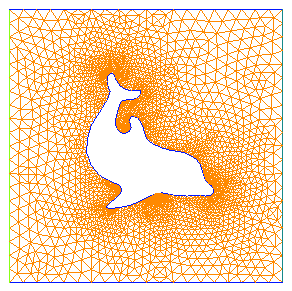
\includegraphics[width=0.75\textwidth]{chapters/elliptic/pics/dolfin_mesh_crop.png}
\caption{An example mesh of a swimming dolphin.}
\label{fig:dolphin}
\end{center}
\end{figure}



Computationally, we need to resort to finite resolutions and this brings us to our third 
challenge. In Figure \ref{fig:dolphin} we see triangulation of domain outside a swimming dolphin. We
can immediately see that it will be difficult to formulate a finite difference approach on this domain
as the nodal points does not form squares. Hence, a stencil like: 
\[
	\frac{u(x+h,y) + u(x,y+y) -4 u(x,y) + u(x-h,y) + u(x, y-h) }{h^2} (\approx \Delta u) 
\]
will not be able to exploit the triangulation. Furhermore, the stencil will cross $\partial \Omega$.   


\section{The finite element method in a nutshell}

The finite element method (FEM) resolves these three challenges by combining 1) the so-called weak formulations
to reduced the demands of differentiability of the solution with 2) 
trial and test functions constructed by the same apporach leads to $N\times N$ matrices and 3)  
a structured approach of integration
adjusted to the underlying meshes. Hence, before we start with FEM, let us recap some fundamental results of calculus that will lead to the weak formulation, the 
Gauss-Green's lemma: 
\begin{equation}
\label{gaussgreen}
\int_\Omega 
-\nabla\cdot(k\nabla u) v \dx =  
\int_\Omega (k\nabla u) \cdot \nabla v \dx  - \int_{\partial \Omega} k\frac{\partial u} {\partial n} v  \ds .  
\end{equation}
Here, we have two functions: the trial function $u$ and the test function $v$, and we are able to move derivatives from $u$ to $v$ and hence reduce the 
strict requirement of $u\in C^2(\Omega)$. 


Next,   
we apply the boundary conditions. That is, for the Dirichlet
condition \eqref{Dirichlet} we already know that $u=g$. Hence, $u$ is not an unknown on that part of the boundary.  Therefore, it is common 
to let $v=0$ at $\partial \Omega_D$. Hence, by inserting the Neumann condition, we obtain that  
\begin{align}
	\int_{\partial \Omega} k\frac{\partial u} {\partial n} v ds &=   
\int_{\partial \Omega_D} k\frac{\partial u} {\partial n} v ds +   \int_{\partial \Omega_N} k\frac{\partial u} {\partial n} v ds  \\   
	&= \int_{\partial \Omega_D} k\frac{\partial u} {\partial n} \, 0 +   \int_{\partial \Omega_N} h v ds   
\end{align}
As such we arrive at the \emph{weak formulation} of the elliptic problem: 
Find $u$ such that 
\begin{equation}
\label{weakform}
\int_\Omega k \nabla u \cdot \nabla v dx = \int_\Omega f v dx + \int_{\Omega_N} h v ds, \quad \forall v  
\end{equation}
Here, we assume as mentioned that $u=g$ and $v=0$ on $\partial \Omega_D$. We will come back to what $\forall v$ means in a 
more precise sense later.  

At this point we \emph{summarize how to obtain a weak formulation} as this will be done over and over again throughout this book.  
First, we multiply with a test function and integrate. Second, the Gauss-Green lemma (or a similar lemma) is applied and third
we apply the boundary conditions. 

\begin{figure}
\begin{center}
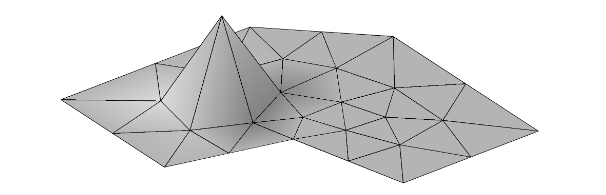
\includegraphics[width=0.75\textwidth]{chapters/elliptic/pics/fem.png}
\caption{One finite element basis function /pyramide function associated with a particular node.}
\label{fig:fembasis}
\end{center}
\end{figure}


\begin{remark}
We remark that the test function $v$ plays the role of pointwise evaluation in the strong formulation \eqref{strong:elliptic}. That is,
we evaluate (or test) the above equation with respect to many different test functions, which in the previous formulation corresponded to many different points. 
We notice that if the test functions are Dirac delta functions then we recover the  strong formulation. However, since but we cannot differentiate the $\delta$ 
functions (in a classical sense) we are only able to evaluate the left-hand side of \eqref{gaussgreen}.  Using the $\delta$ functions as test functions
and avoiding the use of Gauss-Green is often called
the \emph{collocation method} and is used e.g. by the Runge-Kutta method. However, it is 
seldom used for FEM because of the high demands on the differentiability on $u$. 
\end{remark}


The second challenge was to find formulations that lead to linear systems with $N\times N$ matrices. 
The finite element method directly exploits the weak formulation. The finite element method resolves
this challenge by employing the same basis functions for both the trial and the test functions. 
That is, let 
the trial and test functions be as follows:  
\begin{equation}
\label{trialtest}
	u = \sum_{j=1}^N u_j N_j \quad \text{and} \quad v=N_i, \ i=1\ldots N. 
\end{equation}
Here $\{N_i\}$ is a set of basis functions that needs to be choosen somehow. Furthermore, as the third challenge above mentioned, the 
basis functions needs to adapt to a mesh. 
There are many possibilities and one may target the basis function to the problem at hand. 
The simplest basis function is shown in 
Fig \ref{fig:fembasis}. Here, the basis function is chosen as linear functions / pyramides associated with the nodal points, 
so-called Lagrange element of first order.  
There are many, many different finite element functions to choose from and they have different properties. 
Lists of common and unusual elements available in FEniCS can be found in 
\cite{logg2012automated}. 

The FEM problem is obtained by inserting \eqref{trialtest} into the weak formulation \eqref{weakform}, i.e.   
\[
\int_\Omega k \nabla \sum_j u_j N_j  \cdot \nabla N_i dx = \int_\Omega f N_i dx + \int_{\Omega_N} h N_i ds  \quad \forall j .    
\]
We pull the summation out: 
\[
\sum_j u_j  \int_\Omega k \nabla  N_j  \cdot \nabla N_i dx = \int_\Omega f N_i dx + \int_{\Omega_N} h N_i ds \quad \forall j.    
\]
Hence, with  
\begin{eqnarray*}
A_{ij} = \int_\Omega k \nabla  N_j  \cdot \nabla N_i dx, \\  
b_i = \int_\Omega f N_i dx + \int_{\Omega_N} h N_i ds 
\end{eqnarray*}
we arrive at the following linear system 
\[
A u = b 
\]

The following code solves the Poisson problem on the unit square
consisting of $32\times 32$ rectangles, where each rectangle is divided
in two and $f=1$, $g=0$ and $h=x$. Dirichlet conditions are set 
for $y=0$ and Neumann for the rest of $\partial \Omega$.  

\begin{python}
from dolfin import *

# Create mesh and define function space
mesh = UnitSquareMesh(32, 32)
V = FunctionSpace(mesh, "Lagrange", 1)

# Define Dirichlet boundary (x = 0 or x = 1)
def boundary(x): return x[0] < DOLFIN_EPS 

# Define boundary condition
u0 = Constant(0.0)
bc = DirichletBC(V, g, boundary)

# Define variational problem
u = TrialFunction(V)
v = TestFunction(V)
f = Constant(1)
g = Expression("x[0]")
a = inner(grad(u), grad(v))*dx
L = f*v*dx + h*v*ds

# Compute solution
u = Function(V)
solve(a == L, u, bc)

# Save solution in VTK format
file = File("poisson.pvd")
file << u
\end{python}

\section{Brief remark on the strange world of partial differential equations and their discretizations }

A fundamental property in both the theory of partial differential equations and numerical analysis is the
concept of well-posedness. In Hadamard's definition a problem is well-posed if three conditions are met for the given input.  
The solution 1) exists, is 2) unique
and 3) depends continuously on the input. Hence, if we have two inputs to our problem, $b_1$ and $b_2$ 
then the difference between the unique solutions $u_1$ and $u_2$ should be bounded by the differences
between $b_1$ and $b_2$. In terms of linear algebra, we directly obtain well-posedness if
$A$ is a non-singular matrix. That is, we directly obtain 
\[
A(u_1 - u_2)  = (b_1 - b_2)     
\]
which leads to 
\[
	\|(u_1 - u_2) \| = \|A^{-1}(b_1 - b_2)\| \le  \|A^{-1}\| \|b_1 - b_2\|     
\]
and 
\[
	\|(b_1 - b_2) \| = \|A (u_1 - u_2)\|  \le  \|A\| \|u_1 - u_2\|     
\]
Hence, the difference between the solutions $u_1$ and $u_2$ in the sense 
$\|u_1 - u_2\|$ is bounded continuously both above and below by the difference in data in the sense $\|b_1 - b_2\|$.    
In the above, the norms have not been specified, but then, in a finite dimentional setting, all vector norms are equivalent.   
These rather simple observations on the linear algebra level does not easily extend to the continuous setting of partial differential equations. 
For instance, an intuitive estimate given a point $x$ is  
\[
	\|(u_1(x) - u_2(x)) \| = \|(-\Delta)^{-1} \| \|f_1(x) - f_2(x)\|     
\]
This bound is not trivial and in many cases not valid on the continuous level. Here, 

Instead, it is useful to consider the square roots for matrices and operators. 
We will make it more precise later, but let us assume 
that we have a concept of 
$A^{1/2}$ and $A^{-1/2}$. The, as we will see,  the notion 
\[
	\|A^{1/2}(u_1 - u_2) \| = \|A^{-1/2}(b_1 - b_2)\|     
\]
is extraordinary useful and gives precise estimates in a wide range of situations.  
We remark that $\Delta=\nabla\cdot\nabla$ and as such $\nabla$ can be interpreted
as some kind of square root of $\Delta$. There are however some difficulties that
arise with this notion. Let us consider the problem in 1D, using FDM. The stencil 
is then 
\[
- u_{xx} \approx A u =  \frac{-u_{i+1} + 2 u_{i+1}  -u_{i-1}}{h^2}, 
\]  
where $u_i= u(x_i)$ and $x_i = ih, \ i=0,\ldots, N$. 
For a mesh with two internal degrees of freedom, the corresponding matrix 
is 
\[
A = 
\frac{1}{h^2}\begin{pmatrix}
2 & -1 \\ -1 & 2 
\end{pmatrix}
\]
Let $B$ 
\[
B u = 
\frac{1}{h}\begin{pmatrix}
1 & -1 & 0  \\ 0 & 1 & -1  
\end{pmatrix}
\]
Obviously,  
\[
A = B^T B 
\]
However, $B$ is not unique. Furthermore, it is a rectangular matrix that makes
it difficult to invert it. In particular, it has a one-dimentional kernel
consisting of the constant vector $c (1,1,1)^T$, where $c\in \R$. Likewise
in the continuous setting $\nabla$ has a kernel of constant functions.  
However, and withough any mathematical rigour, 
the correct and actually quite practical 
variant of the above estimate is    
\[
\|\nabla (u_1 - u_2) \| = \|\nabla^{-1}(f_1 - f_2)\|     
\]
We do however need to make sense of the 
$\nabla^{-1}$. For now it is enough to think of it as some form of antiderivative. 
Here, for instance $u_1, f_1$ may be the actual continuous solution and input data whereas the 
$u_2, f_2$ are the numerical solution and input data. 

\section{Further reading}
There are several execellent and highly recommended books on the finite element method~\cite{braess2007finite, brenner2008mathematical}. 


\section{Exercises}

\begin{exercise}
Consider the problem $-u''(x) = x^2$ on the unit interval with $u(0) = u(1) = 0$.  
Let $u=\sum_{k=1}^{10} u_k \sin(\pi k x )$ and $v=\sin(\pi l x)$ for $l=1, \ldots 10$
and solve \eqref{weakform}. What is the error in $L_2$ and $L_\infty$.  
\end{exercise}

\begin{exercise}
Consider the same problem as in the previous exercise, but using Bernstein polynomials. 
That is, the basis for the Bernstein polynomial of order 10 on the unit interval is $B_k(x)=x^k(1-x)^{10-k}$ for $k=0, \ldots, 10$.  
Let $u=\sum_{k=0}^{10} u_k B_k(x )$ and $v=B_l(x)$ for $0=1, \ldots 10$
and solve \eqref{weakform}. What is the error in $L_2$ and $L_\infty$.  
\end{exercise}

\begin{exercise}
Consider the same problem as in the previous exercise, but with  
$-u''(x) = sin(k \pi x)$ for $k=1$ and $k=10$.  
\end{exercise}

\begin{exercise}
Consider the same problem as in the previous exercise, but
with the finite element method in for example FEniCS, using Lagrange 
method of order 1, 2 and 3. 

\end{exercise}












\chapter{Crash course in Sobolev Spaces}

\label{chap-sobolev}
\section{Introduction}

Sobolev spaces are fundamental in the analysis of partial differential equations and also for 
finite element methods. Many books provide a detailed and comprehensive analysis of these spaces
that in themselves deserve significant attention if one wishes to understand the foundation that
the analysis of partial differential equations relies on. In this chapter we will however not
provide a comprehensive mathematical description of these spaces, but rather try to provide 
insight into their use. 

We will here provide the definition of these spaces. Further we will show typical functions, useful
for finite element methods,  that are in some but not all spaces. We also show how different norms
capture different characteristics.   

\section{Norms, inner products and Sobolev spaces}

Sobolev spaces are generalizations of $L^p$ spaces. $L^p$ spaces are function spaces defined as follows.  
Let $u$ be a scalar valued function on the domain $\Omega$, which for 
the moment will be assumed to be the unit interval $(0,1)$. Then the $L^p$ norm on $\Omega$ is:    
\[
\|u\|_p = (\int_0^1 |u|^p \, dx)^{1/p} .    
\]
$L^p(\Omega)$ consists of all functions for which $\|u\|_p < \infty$. 
Sobolev spaces generalize $L^p$ spaces by also including the derivatives.  
On the unit interval, the $W^{k,p}$ norm is defined as  
\begin{equation}
\label{Wpk}
\|u\|_{k,p} = (\int_\Omega \sum_{i \le k} |(\frac{\partial^i u}{\partial x^i}) |^p \, dx)^{1/p} .    
\end{equation}
Then the Sobolev space $W^p_k(\Omega)$ consists of 
all functions with $\|u\|_{p,k} < \infty$. $W^p_k$ is a so-called Banach space - that is 
a complete\footnote{We will not go into the details of complete spaces in this book, but remark that
the space of real numbers is complete, while the space of rational numbers is not. } normed vector space. 
The corresponding semi-norm, that only include the highest order derivative is 
\begin{equation}
\label{semiWpk}
|u|_{k,p} = (\int_\Omega  |(\frac{\partial^k u}{\partial x^k})   u|^p \, dx)^{1/p} .    
\end{equation}
The case $p=2$ is special in the sense that not only a norm is defined but also an inner product.    
The Banach space then forms a Hilbert space and these named with $H$ in Hilbert's honor. 
That is $H^k(\Omega) = W^{2,k}(\Omega)$. The inner product between the functions $u$ and $v$ is:  
\[
(u, v)_{k} = \sum_{i \le k} \int_\Omega \frac{\partial^i u}{\partial x^i} \frac{\partial^i v}{\partial x^i} \,  dx.    
\]

For the most part, we will employ the two spaces $L^2(\Omega)$ and $H^1(\Omega)$, but also other
spaces will be used from time to time.  
The difference between the norm in $L^2(\Omega)$ and $H^1(\Omega)$ is illustrated in the following example.   

\begin{example}{Norms of $sin(k \pi x)$} \label{sc:ex1} 
Consider the functions $u_k = \sin(k \pi x)$ on the unit interval. Figure \ref{fig:sin} shows the function for $k=1$ and $k=10$. Clearly, the $L^2$ and $L^7$ behave similarly in the sense
that they remain the same as $k$ increases. On the other hand, the $H^1$ norm of $u_k$
increases dramatically as $k$ increases. The following code shows how the 
norms are computed using FEniCS.         

\begin{python}
from dolfin import *

N = 10000 
mesh = UnitInterval(N)
V = FunctionSpace(mesh, "Lagrange", 1)

for k in [1, 100]: 
  u_ex = Expression("sin(k*pi*x[0])", k=k)
  u = project(u_ex, V)

  L2_norm = sqrt(assemble(u**2*dx))
  print "L2 norm of sin(%d pi x) %e " % (k, L2_norm) 

  L7_norm = pow(assemble(abs(u)**7*dx), 1.0/7)
  print "L7 norm of sin(%d pi x) %e " % (k, L7_norm) 

  H1_norm = sqrt(assemble(u*u*dx+inner(grad(u), grad(u))*dx))
  print "H1 norm of sin(%d pi x) %e" % (k, H1_norm) 
\end{python}

\begin{table}[h]
\begin{center}
\begin{tabular}{|c|c|c|c|}  \hline
$k \backslash norm $ & $L^2$ &   $L^7$ &  $H^1$ \\ \hline
1 & 0.71 &    0.84   & 2.3      \\ \hline
10  & 0.71 &   0.84    & 22    \\ \hline
100  & 0.71 &   0.84  &  222   \\ \hline
\end{tabular}
\caption{ The $L^2$, $L^7$, and $H^1$ norms of $sin(k \pi x)$ for k=1, 10, and 100.   }
\label{norms}
\end{center}
\end{table}


\end{example}



\begin{figure}
\label{fig:sin}
\begin{center}
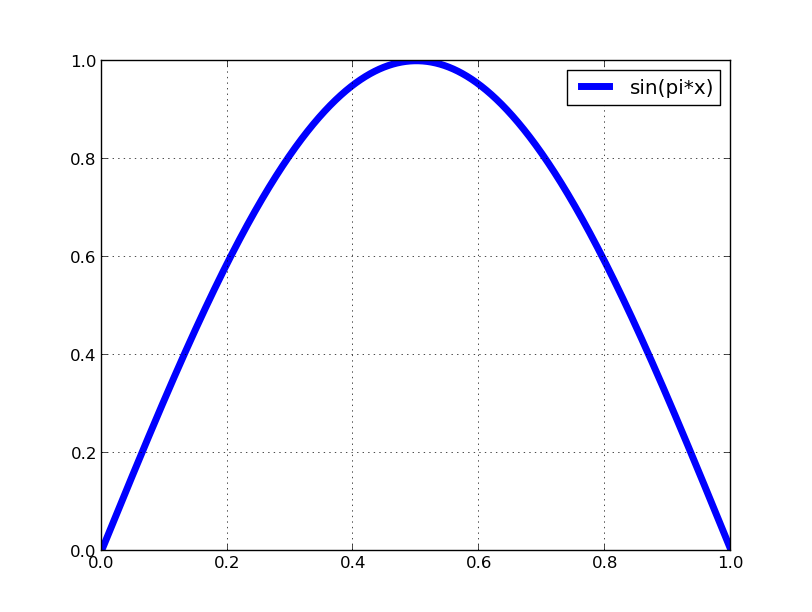
\includegraphics[width=5cm]{chapters/SobolevCrash/sin.png}
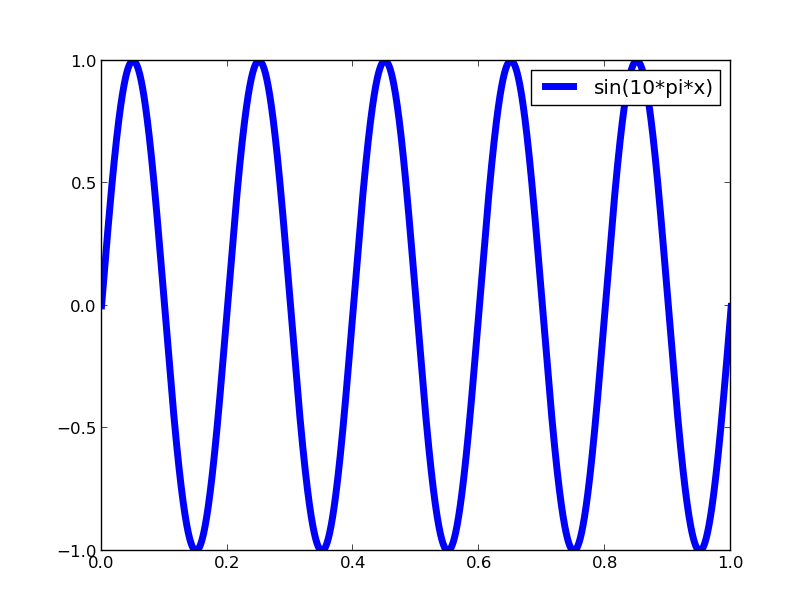
\includegraphics[width=5cm]{chapters/SobolevCrash/sin10.png}
\caption{Left picture shows $\sin(\pi x)$ on the unit interval, while 
the right picture shows $\sin(10 \pi x)$. }\label{fig:sin}
\end{center}
\end{figure}


\section{Spaces and sub-spaces, norms and semi-norms}

The Sobolev space with $k$ derivatives in $L_2(\Omega)$ was denoted by $H^k(\Omega)$. The subspace
of $H^k$ with $k-1$ derivatives equal to zero at the boundary is denoted 
$H^k_0(\Omega)$. For example, $H^1_0(\Omega)$ consists of all functions in $H^1$ that are zero 
at the boundary. Similarly, we may also defined a subspace  
$H^1_g(\Omega)$ which consists of all functions in $H^1(\Omega)$ that are equal to the function $g$ 
on the boundary. 

The norm $\|\cdot\|_{p,k}$ defined in \eqref{Wpk} is a norm
which means that $\|u\|_{p,k} > 0$ for all $u\not=0$.    
On the other hand  $|\cdot|_{p,k}$ is a semi-norm, meaning 
that $|u|_{p,k} \ge  0$ for all $u$.   
The space $H^1(\Omega)$ is defined by the norm 
\[
\|u\|_1 = (\int_\Omega u^2 + (\nabla u)^2 \, dx)^{1/2}  
\]
and contains all functions for which $\|u\|_1 \le \infty$. 
Often we consider subspaces of $H^1$ satisfying the Dirichlet boundary conditions. 
The most common space is denoted $H^1_0$. This space contains all functions 
in $H^1$ that are zero on the boundary.  
The semi-norm $|\cdot|_1$ defined as 
\[
|u|_1 = (\int_\Omega  (\nabla u)^2 \, dx)^{1/2}  
\]
is a norm on the subspace $H^1_0$. In fact, as we will see later, Poincare's lemma
ensures that $\|\cdot\|_1$ and  $|\cdot|_1$ are equivalent norms on $H^1_0$ (see Exercise \ref{ex:poincare}).  





\section{Examples of Functions in Different Spaces}

The above functions $\sin(k \pi x)$ are smooth functions
that for any $k$ are infinitely many times differentiable. 
They are therefore members of any Sobolev space. 

On the other had, the step function in upper picture in Figure \ref{fig:piecewise} is 
discontinuous in $x=0.2$ and $x=0.4$. Obviously, the function is in $L^2(0,1)$, but 
the function is not in $H^1(0,1)$ since the derivative of the function  consists of Dirac's 
delta functions\footnote{The Dirac's delta function $\delta_x$ is 0 everywhere except at 
$x$ where it is  $\infty$ and $\int_\Omega \delta_x \, dx = 1$. Hence, 
Dirac's delta function is in $L^1(\Omega)$ but not in $L^2(\Omega)$.  
} 
that are $\infty$ at $x=0.2$ and 
$-\infty$ in $x=0.4$. 

The hat function in the lower picture in Figure \ref{fig:piecewise} is a typical
first order finite element function. The function is in both $L^2(0,1)$ and $H^1(0,1)$ (see
Exercise \ref{ex:piecewise}).         
In general, functions in $H^q(0,1)$ are required to be in $C^{q-1}(0,1)$, where $C^k(0,1)$ is the
class  where the $k$'th derivatives exist and
are continuous on the unit interval.   

\begin{remark}
In $C^k(\Omega)$ a function and its $k$ derivatives can be evaluated at any given point in $\Omega$ and  
the result will be a finite value. How about functions in $H^k(\Omega)$? In general only functions
in $H^k(\Omega)$ for $k\ge 2$ allow pointwise evaluation. The exact relationship between 
continous functions and Sobolev spaces are covered by the  Sobolev Embedding Theorem, which will not 
be covered in this book. 
Anyways, in $L^2(\Omega)$ or $H^1(\Omega)$ we should make note and be careful when we perform pointwise evaluations. 
\end{remark}


\begin{figure}
\begin{center}
%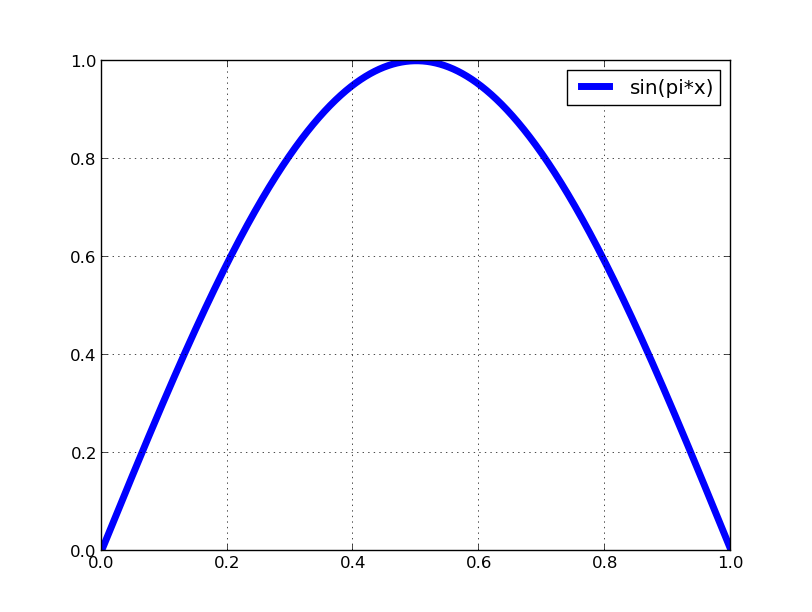
\includegraphics[width=6cm]{chapters/SobolevCrash/sin.png}
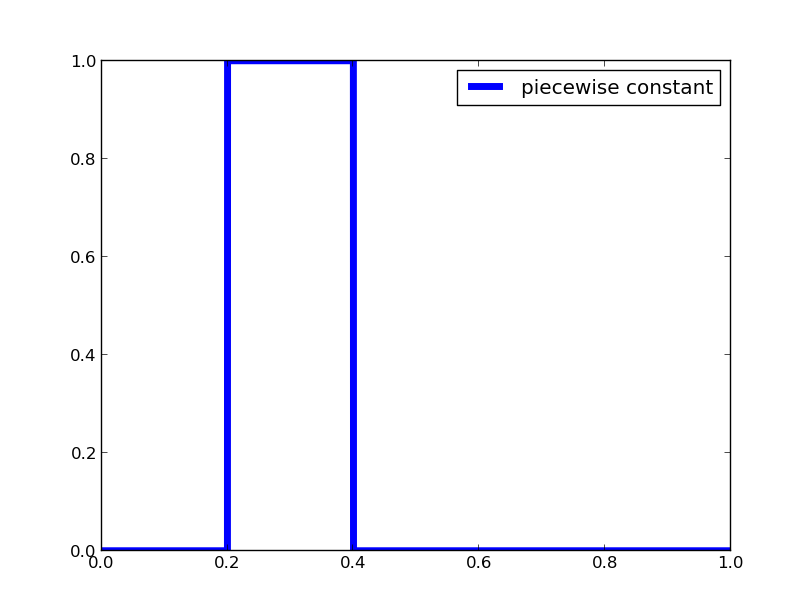
\includegraphics[width=6cm]{chapters/SobolevCrash/pc.png}
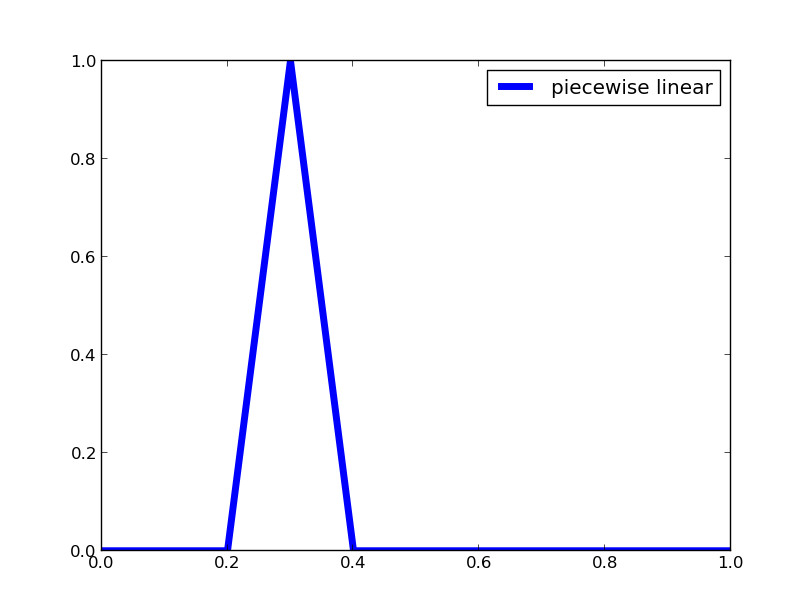
\includegraphics[width=6cm]{chapters/SobolevCrash/pl.png}
\caption{The upper picture shows a piecewise function, discontinuous at $x=0.2$ and $x=0.2$, while
the lower picture shows a linear function that is continuous. }  
\label{fig:piecewise}
\end{center}
\end{figure}

\section{Sobolev Spaces and Polynomial Approximation}
From Taylor series approximation we know that  $f(x+h)$ may be approximated
by $f(x)$ and a polynomial in $h$ that depends on the derivatives of $f$. 
To be precise, 
\[
|f(x+h) - P_{h,k} f (x) |  \le  \mathcal{O}(h^{k+1}) .    
\]
Here, $P_{h,k} f(x)$ is the following polynomial of degree $k$ in $h$, 
\[
P_{h,k} f(x) = f(x) + \sum_{n=1}^k \frac{f^{(n)}(x)}{n!} h^n . 
\]
where $f^{(n)}$ denotes the $n$'th derivative of $f$. 

In general, approximation by Taylor series bears strong requirement on the smoothness 
of the solution which needs to be differentiable in a point-wise sense.   
Hence, we need to defined the polynomials in an alternative way, but the
results are similar.  We conclude, without proof, that  in Sobolev spaces we have the very useful approximation property  
\begin{equation}
\label{bramblehilbert}
|u - P_m u|_{k,p} \le C h^{m-k} |u|_{m,p} \quad \mbox{ for } k=0,\ldots,m \mbox{ and }  p\ge 1. 
\end{equation}
This property is used extensively in analysis of finite element methods and
is called the Bramble-Hilbert lemma for $k\ge 2$. The case $k=1$ was included by a special interpolation operator by 
Clement, the so-called Clement interpolant. 
For proof, see e.g. \cite{braess2007finite, brenner2008mathematical}.  




\section{Eigenvalues and Finite Element Methods}
\label{sec:eig and fem}

It is well known that for $-\Delta$  with homogenous Dirichlet conditions on the unit
interval $(0,1)$, 
the eigenvalues 
and eigenvectors
are $(\pi k)^2$ and $sin(\pi k x)$, $k=1, \ldots, \infty$, respectively. 
It is natural to expect that the eigenvalues in the discrete setting
approximate the continuous eigenvalues such that 
the minimal eigenvalue is $\approx \pi^2$, while the maximal eigenvalue
is $\approx \pi^2 /h^2$, where $k=1/h$ is the largest $k$ that may be represented
on a mesh with element size $h$.  
Computing the eigenvalues of the finite element stiffness matrix in FEniCS as\footnote{
We use the \emp{assemble\_system} function to enforce the Dirichlet
condition in symmetric fashion.}, 
\begin{python}
A = assemble_system(inner(grad(u), grad(v))*dx, Constant(0)*v*dx, bc)
\end{python}
reveals that the eigenvalues are differently scaled. In fact, the minimal 
eigenvalue is $\approx \pi^2 h$ and that the maximal eigenvalue is  $\approx \pi^2/h$.      
The reason is that the finite element method introduces a mesh-dependent 
scaling due to the fact that it is a variational method. 
Specifically, if we want to approximate a $f$ as $\sum_j f_j N_j$ we notice
that we may calculate $f_j$ in a variational sense as follows: 
\[
 \sum_j \int_\Omega f_j N_j N_i \, dx = \int_\Omega f N_i \, dx   
\]
Hence, we notice here that, we are solving a linear system
\[
	M f = b, \mbox{ with } M_{ij} = \int_\Omega N_j N_i \, dx \mbox{ and } b_i = \int_\Omega f N_i \, dx  
\]
Both $\{f_i\}_i$ and $\{b_i\}_i$ are representations of $f$, often called the nodal and dual representations~\cite{mardal2011preconditioning}. They scale differently since
the entries of the mass matrix scale with the size of the elements in the mesh. 

To estimate the continuous eigenvalues, we  need to make sure that both the left- and right-hand sides are in the same representation, either nodal
or dual. Hence, we consider the generalized eigenvalue problem, 
\begin{equation} 
\label{geneig}
A x = \lambda M x,   
\end{equation} 
where $A$ is the above mentioned stiffness matrix and $M$ is the mass
matrix (or the finite element identity matrix) 
\begin{python}
M = assemble_system(inner(u*v*dx, Constant(0)*v*dx, bc)
\end{python}

Figure \ref{geneig} shows the eigenvalues of $-\Delta$, $A$, and  
\eqref{geneig} based on the following code: 
\begin{python}
from dolfin import *
import numpy
from scipy import linalg, matrix

def boundary(x, on_boundary): return on_boundary

for N in [100, 1000]: 
  mesh = UnitIntervalMesh(N)
  V = FunctionSpace(mesh, "Lagrange", 1)
  u = TrialFunction(V)
  v = TestFunction(V)

  bc = DirichletBC(V, Constant(0), boundary)
  A, _ = assemble_system(inner(grad(u), grad(v))*dx, Constant(0)*v*dx, bc)
  M, _ = assemble_system(u*v*dx, Constant(0)*v*dx, bc)

  AA = matrix(A.array())
  MM = matrix(M.array())

  k = numpy.arange(1, N, 1)
  eig = pi**2*k**2 

  l1, v  = linalg.eigh(AA)
  l2, v  = linalg.eigh(AA, MM)

  print "l1 min, max ", min(l1), max(l1) 
  print "l2 min, max ", min(l2), max(l2) 
  print "eig min, max ", min(eig), max(eig) 

  import pylab 
  pylab.loglog(l1[2:], linewidth=5) # exclude Dirichlet values 
  pylab.loglog(l2[2:], linewidth=5) # exclude again 
  pylab.loglog(eig, linewidth=5)
  pylab.legend(["eig(A)", "eig(A,M)", "cont. eig"], loc="upper left")
  pylab.show()
\end{python}

\begin{figure}
\begin{center}
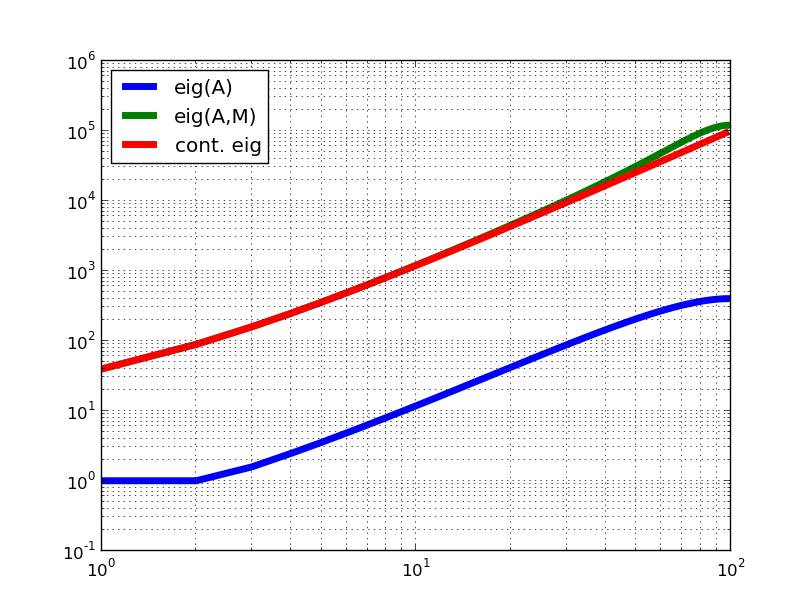
\includegraphics[width=6cm]{chapters/SobolevCrash/eig.png}
\caption{A log-log plot of the eigenvalues of $A$, $M^{-1} A$, and $-\Delta$. }  
\label{fig:geneig}
\end{center}
\end{figure}
From Figure \ref{fig:geneig} we see that that the eigenvalues
of \eqref{geneig} and $-\Delta$ are close, while the eigenvalues
of $A$ is differently scaled.  
We remark that we excluded the two smallest eigenvalues in the discretized problems 
as they correspond to the Dirichlet conditions. 
%We remark 
%that we use \emp{pytave}, the Python interface of Octave because
%\emp{numpy} is not trustworthy for eigenvalue computations on 
%"large" linear systems. A description of \emp{pytave} is found in~\cite{mardal2013combining}.  


\section{Boundary conditions, Traces and Fractional Sobolev Spaces }

In order to make sense of for instance boundary conditions we need to 
restrict from a domain $\Omega$ to $\partial \Omega$. Hence, for instance
if $\Omega$ is the unit square in 2D then $\partial \Omega$ consists of the 1D lines that 
connect the vertices at the boundary of the unit square. However, a 
1D line is inifinitely thin and has no measure in 2D. In Sobolev spaces, which
have extra smoothness in terms of the extra derivatives, the   
values at lower dimentional manifolds may be used. In fact, their use is required 
in terms of boundary conditions. In order to make sense of values at lower 
dimensional manifolds we need the mathematical constructs of traces and fractional 
Sobolev spaces. Specifically, let $T:\Omega \rightarrow \partial \Omega$ be the 
the so-called trace operator and $u \in H^k(\Omega)$ then 
$Tu \in H^{k-1/2} (\partial \Omega)$. Typically, when finite element methods
are used for single-physics problems then there is no need to pay attention to 
the fractional norms when implementing the boundary conditions. Boundary conditions
are assigned at the boundary in a straightforward way as will be discussed in the next
chapter. However, for multi-physics problems, care may be required for efficient and
accurate simulation.   

\section{Negative and Fractional Norms}

As will be discussed more thoroughly later, 
$-\Delta$ is a symmetric positive operator and can be thought of 
as an infinite dimensional matrix that is symmetric and positive.  
It is also know from Riesz representation theorem that if
$u$ solves the problem
\begin{eqnarray*}
-\Delta u &=& f, \quad \mbox{ in } \Omega, \\   
        u &=& 0, \quad \mbox{ on } \partial \Omega  
\end{eqnarray*}
then 
\begin{equation}
\label{riesz}
|u|_1 = \|f\|_{-1} . 
\end{equation}
This implicitly define the $H^{-1}$ norm, although
the definition then requires the solution of a Poisson problem.   
For example, in the previous example where
$u_k = sin(k\pi x)$, we  have already estimated  
that $|u_k|_1 = \frac{\pi k}{\sqrt{2}}$ and therefore 
$\|u_k\|_{-1} = |(-\Delta)^{-1} u_k|_1 = \frac{1}{\sqrt{2} k \pi }$.  
We notice that the $\|\cdot\|_1$ norm weights high frequency oscillations heavily (linear in $k$), whereas
the $\|\cdot\|_{-1}$ does not (it scales as $1/k$). On the other hand $L^2$ weights oscillations at all frequencies
equally.   \label{sinkpnorms} 

Let us now generalize these considerations and  consider a matrix 
(or differential operator) $A$ which is
symmetric and positive. $A$ has positive and real
eigenvalues and defines an inner product which may
be represented in terms of eigenvalues and eigenfunctions. Let     
$\lambda_i$ and $u_i$ be the eigenvalues and eigenfunctions
such that 
\[
A u_i = \lambda_i u_i  
\]
Then, $x$ may be expanded in terms of the eigenfunctions $u_i$ as
$x=\sum_i c_i u_i$, where $c_i = (x, u_i)$,  and we obtain 
\[
(x,x)_A = (A x, x) = (A \sum_i c_i u_i  , \sum_j c_j u_j)     
= (\sum_i \lambda_i  c_i u_i  , \sum_j c_j u_j)  
\]
Because $A$ is symmetric, the egenfunctions $u_i$  are orthogonal to each other
and we may choose a normalized basis such that $(u_i, u_j) =  \delta_{ij}$.
With this normalization, we simply obtain
\[
\|x\|_A^2 = (x,x)_A = (A x, x) = (A \sum_i c_i u_i  , \sum_j c_j u_j)     
= \sum_i \lambda_i  c_i^2    
\]


A generalization of the $A-$inner product (with corresponding norm) to 
a $A^q-$inner product that allow for both negative and franctional $q$  
is then as follows
\begin{equation}
\label{qnorm}
\|x\|_{A,q}^2 =  (x,x)_{A,q} =  \sum_i \lambda^q_i c_i^2.     
\end{equation}
Clearly, this definition yields 
that $|u_k|_1 = \frac{\pi k}{\sqrt{2}}$ and 
$\|u_k\|_{-1} = \frac{1}{\sqrt{2} k \pi }$, as above.  

As mentioned in Section \ref{sec:eig and fem}, 
care has to be taken in finite element methods if the discrete eigenvalues
are to correspond with the continuous eigenvalues. We will therefore detail
the computation of negative and fractional norms in the following.   
Let $\lambda_i$ and $u_i$ be the eigenvalues and eigenvectors of the following
generalized eigenvalue problem  
\begin{equation}
\label{gen_eig}
A u_i = \lambda_i M u_i 
\end{equation}
and let $U$ be the matrix with the eigenvectors as columns. 
The eigenvalues are normalized in the sense 
that 
\[
U^T M U = I 
\]
where $I$ is the identity matrix. 
We obtain 
\[
U^T A U = \Lambda \quad \mbox{ or } \quad A = M U \Lambda (M U)^T  ,  
\]
where $\Lambda$ is a matrix with the eigenvalues $\lambda_i$ on the diagonal.  
Hence also in terms of the generalized eigenvalue problem \eqref{gen_eig}
we obtain the $A-$norm as  
\[
\|x\|^2_A = x^T MU \Lambda (MU)^T x   
\]
and  
we may define fractional and negative norms in the same manner
as \eqref{qnorm}, namely that 
\[
\|x\|^2_{A,M,q} = x^T M U \Lambda^q (MU)^T x .     
\]

Defining negative and fractional norms in terms of eigenvalues and eigenvectors 
is convenient for small scale problems, but eigenvalue problems are computationally
demanding. It may, however, be tractable on subdomains, such as surfaces or interfaces 
of larger problems. There are however more    
efficient was of computing such norms and operators, but those are beyond the scope of this
book. 


\begin{example}{Computing the $H^1$, $L^2$, and $H^{-1}$ norms} \label{sc:ex2} 

Let us consider $\Omega = (0,1)$ and $u_k = sin(\pi k x)$.  
Table \ref{norms} shows the $H^1$, $L^2$, and $H^{-1}$ norms as computed
with \eqref{qnorm} with $q=1, 0$, and $-1$, respectively.  Comparing 
the computed norms with the norms $L^2$ and $H^1$ norms  computed
in Example \ref{sc:ex1}, or analytically on page \pageref{sinkpnorms}  we see that the above definition \eqref{qnorm}
reproduces the $H^1$ and $L^2$ norms with $q=1$ and $q=0$, respectively.     
We also remark that while the $H^1$ norm increases as
$k$ increases, the  $H^{-1}$ norm demonstrates a corresponding decrease.  
Below we show the code for computing these norms. 


\begin{table}[h]
\begin{center}
\begin{tabular}{|c|c|c|c|}  \hline
$k \backslash norm $ & $H^1, \ q=1  $ &   $L^2, \ q=0$ &  $H^{-1}, \ q=-1$ \\ \hline
1 &  2.2 &    0.71  &  0.22      \\ \hline
10  & 22 &    0.71   & 0.022   \\ \hline
100  & 222 &   0.71  & 0.0022   \\ \hline
\end{tabular}
\caption{ The $L^2$, $L^7$, and $H^1$ norms of $sin(k \pi x)$ for k=1, 10, and 100.   }
\label{table:norms}
\end{center}
\end{table}


\begin{python}
from dolfin import *
from numpy import matrix, diagflat, sqrt
from scipy import linalg, random 

def boundary(x, on_boundary): return on_boundary

mesh = UnitIntervalMesh(200)
V = FunctionSpace(mesh, "Lagrange", 1)
u = TrialFunction(V)
v = TestFunction(V)
bc = DirichletBC(V, Constant(0), boundary)

A, _ = assemble_system(inner(grad(u), grad(v))*dx, Constant(0)*v*dx, bc)
M, _ = assemble_system(u*v*dx, Constant(0)*v*dx, bc)
AA = matrix(A.array())
MM = matrix(M.array())

l, v = linalg.eigh(AA, MM)
v = matrix(v)
l = matrix(diagflat(l))

for k in [1, 10, 100]: 
  u_ex = Expression("sin(k*pi*x[0])", k=k)
  u = interpolate(u_ex, V)
  x = matrix(u.vector().array())

  H1_norm = pi*k*sqrt(2)/2  
  print "H1 norm of sin(%d pi x) %e (exact)          " % (k, H1_norm) 
  H1_norm = sqrt(assemble(inner(grad(u), grad(u))*dx)) 
  print "H1 norm of sin(%d pi x) %e (|grad(u)|^2)    " % (k, H1_norm) 
  H1_norm = sqrt(x*AA*x.T)    
  print "H1 norm of sin(%d pi x) %e (x A x' )        " % (k, H1_norm) 
  W = MM.dot(v)
  H1_norm = sqrt(x*W*l*W.T*x.T)   
  print "H1 norm of sin(%d pi x) %e (eig)            " % (k, H1_norm) 

  print "" 

  L2_norm = sqrt(2)/2 
  print "L2 norm of sin(%d pi x) %e (exact)          " % (k, L2_norm) 
  L2_norm = sqrt(assemble(u**2*dx)) 
  print "L2 norm of sin(%d pi x) %e   |u|^2          " % (k, L2_norm) 
  L2_norm = sqrt(x*MM*x.T) 
  print "L1 norm of sin(%d pi x) %e (x M x' )        " % (k, L2_norm) 
  W = MM.dot(v)
  L2_norm = sqrt(x*W*l**0*W.T*x.T)   
  print "L2 norm of sin(%d pi x) %e (eig)            " % (k, L2_norm) 

  print "" 

  Hm1_norm = sqrt(2)/2/k/pi  
  print "H^-1 norm of sin(%d pi x) %e (exact)        " % (k, Hm1_norm) 
  Hm1_norm = sqrt(x*W*l**-1*W.T*x.T)  
  print "H^-1 norm of sin(%d pi x) %e (eig)          " % (k, Hm1_norm) 
  Hm1_norm = sqrt(x*MM*linalg.inv(AA)*MM*x.T)    
  print "H^-1 norm of sin(%d pi x) %e (x inv(A) x') " % (k, Hm1_norm) 
\end{python}

\end{example}


\begin{remark}{\textbf{Norms for $|q| > 1$.} } \\
The norm \eqref{qnorm} is well defined for any $|q|$ > 1, but will not 
correspond to the corresponding Sobolev spaces.    
\end{remark}

\begin{remark}{\textbf{The standard definition of a dual norm}} \\
\label{dualnorm}
Let $(\cdot, \cdot)_A$ be an inner product over the Hilbert
space $V$.  The norm of the dual space is then defined by 
\[
\|f\|_{A^*} = \sup_{v\in V} \frac{(f,v)}{(v,v)_A} .    
\]
For example, the $H^{-1}$ norm is defined as 
\[
\|f\|_{-1} = \sup_{v\in H^1} \frac{(f,v)}{(v,v)_1} .    
\]


\end{remark}

\section{Exercises}

\begin{exercise}
What is a norm? Shown that 
\[
\|u\|_p = (\int_\Omega |u|^p \, dx)^{1/p} .    
\]
defines a norm on $L^p(\Omega)$. 

\end{exercise}

\begin{exercise}
What is an inner product? 
Show that 
\[
	(u, v)_{k} = \sum_{i \le k} \int_\Omega (\frac{\partial u}{\partial x})^i (\frac{\partial v}{\partial x})^i \,  dx.    
\]
defines an inner product on $H^1_0 (\Omega)$ for $\Omega=(0,1)$.   

\end{exercise}

\begin{exercise}
Compute the $H^1$ and $L^2$ norms of a random function with values
in $(0,1)$ on meshes representing the unit interval of with $10$, $100$, and $1000$ cells.   
\end{exercise}

\begin{exercise}
Compute the $H^1$ and $L^2$ norms of  $\sin( k \pi x)$ on the unit interval analytically 
and compare with the values presented in Table \ref{table:norms}.   
\end{exercise}

\begin{exercise}
\label{ex:piecewise}
Compute the $H^1$ and $L^2$ norms of  the hat function in Picture \ref{fig:piecewise}.   
\end{exercise}



\begin{exercise}
\label{ex:hat2}
Consider the following finite element function $u$ defined
as  
\[
u = \Bigg\{ 
\begin{array}{ll} \frac{1}{h} x - \frac{1}{h} (0.5 - h), & x=(0.5-h,0.5) \\  
              -\frac{1}{h} x + \frac{1}{h} (0.5 - h),  & x=(0.5,0.5 + h) \\  
                0, & \mbox{elsewhere}  
\end{array}
\]
That is, it corresponds to the hat function in Figure \ref{fig:piecewise}, where
$u(0.5)=1$ and the hat function is zero every where in $(0,0.5-h)$ and  $(0.5+h, 1)$.  
Compute the $H^1$ and $L^2$ norms of this function analytically, and the 
$L^2$, $H^1$ and $H^{-1}$ norms numerically for $h=10$, $100$ and $1000$.    
\end{exercise}







\chapter{Some common finite elements}
\label{element}

\section{Introduction}

There is a jungle of finite elements that have been invented in the early 1940s, and we
will not here give a comprehensive description of the topic. Instead, we will try to motivate
the method by rather simple examples before we discuss some of the general features. 
The formal definition of a finite element~\cite{ciarlet2002finite}: 

\begin{defin}
A finite element is defined by a triplet $(T, V, L)$, where 
\begin{itemize}
\item $T$ is a bounded domain in $\mathbb{R}^d$, most typically a polyhedron; 
\item $V = \{\psi_i\}_{i=1}^n$ is a set of linearly independent basis functions on $T$; 
\item $D = \{d_i\}^n_{i=1}$ is a set of $n$ (linearly independent) 
  degrees of freedom (formally bounded linear functionals on $T$) 
\end{itemize}
\end{defin}
As we see, the term "finite element" refers not only to the cells of the mesh, but also the function space and associated degrees of freedom. The definition is quite abstract, but as we will see, the definition encapsulate precisely what is needed in order to definite a numerical method on a mesh. 

Most commonly, a \emp{nodal basis} is defined as follows 
\begin{defin}
\label{nodal:basis}
The nodal basis for the triplet  $(T, V, L)$ is defined as the set of basis functions
$\{\phi_i\}^n_{i=1}$ that satisfies  
\[
d_j(\phi_i) = \delta_{ij}, \quad for 1 \le i,j \le n. 
\]
The $\{d_j\}^n_{i=1}$ is often called the dual basis of the finite element.  
\end{defin}

\section{Some example finite elements: Lagrange and Hermite on the unit interval. }
Let us now try to make this concrete in a couple of simple examples. First we notie that  
in the above, we have two function spaces $\{\psi_i\}$ and $\{\phi_i\}$. Clearly, 
\[
\phi_i = \sum \alpha_{ij}\psi_j,  
\]
where the matrix $\alpha_{ij}$ is determined such that 
\[
d_i(\phi_j) = \delta_{ij}. 
\]
Hence, let then $V=\mathbb{P}_k$ and lets consider the Lagrange and Hermite elements, defined in terms
of Lagrange and Hermite interpolation, respectively.  
On the unit interval
\[
\mathbb{P}_k = \{1, x, \ldots, x^k\}. 
\]
Clearly, $\mathbb{P}_k$ has $k+1$ basis functions  and they are all linearly independent. 
The Lagrange and Hermite elements are then defined in the examples below. 
\begin{exmp}[\textbf{The Lagrange element in 1D.}]
\label{lagrange:element}
Lagrange interpolation is defined simply by nodal values in a set of points. Hence, 
let 
\[
x_j = j \Delta x, \quad \Delta x = \frac{1}{k}, \quad  j= 0, \dots, k 
\]
Then the j'th Lagrange function $L_j$ can be written as a linear combination the basis of $\mathbb{P}_k$ as 
\[ 
L_j = \sum_i \alpha_{ij} x^i 
\]
where $\alpha_{ij}$ are determined by 
\[ 
d_i(L_j) = L_j(x_i) = \delta_{ij} . 
\]
In 1D, an explicit formulation can be derived for $L_j$, namely 
\[
L_j(x) = \frac{x-x_0}{x_j-x_0} \ldots \frac{x-x_{j-1}}{x_j-x_{j-1}} \ldots \frac{x-x_{j+1}}{x_j-x_{j+1}} \ldots \frac{x-x_k}{x_j-x_k}  
\]
Clearly, for instance $L_j(x_0) = 0$ whereas  $L_j(x_j) = 1$.  
\end{exmp}
Calculating the basis for a Lagrange element yields and explicit formula in 1D, but is harder in higher dimensions.
The following code computes the basis directly from the abstract definition without references to the above formula, using SymPy.  
\begin{python}
from sympy import * 

def dirac(i,j): 
  if i == j: return 1 
  else: return 0 

k = 5  
x = Symbol("x") 
dx = 1/k 

basis = [x**j for j in range(0, k+1)] 
points = [j*dx for j in range(0, k+1)] 
dofs = symbols("a:%d"%(k+1))

print ("A basis for the polynomial space ", basis) 
print ("A set of points to use for computing the nodal basis ", points) 
print ("The degrees of freedom, represented as symbols ", dofs) 

pol = sum([dofs[i]*basis[i] for i in range(0, (k+1))])   
print ("A generic function is then ", pol)

Lagrange_basis = []
for i in range(0, (k+1)): 
  equations = []
  for j in range(len(points)):  
    p = points[j]
    eq = pol.subs(x,p) - dirac(i,j) 
    equations.append(eq)
  coeff = solve(equations, dofs) 
  Nj = pol.subs(coeff)
  Lagrange_basis.append(Nj) 

print (Lagrange_basis) 

# check that the Lagrange basis is what it is supposed to be 
for i, basis in enumerate(Lagrange_basis): 
    for j, point in enumerate(points): 
        print ("i,j ", i,j, " basis evaluation ",  "%0.3f" % basis.subs({ x: point})) 
\end{python}
The output is as follows: 
\begin{python}
A basis for the polynomial space  [1, x, x**2, x**3, x**4, x**5]
A set of points to use for computing the nodal basis  [0.0, 0.2, 0.4, 0.6000000000000001, 0.8, 1.0]
The degrees of freedom, represented as symbols  (a0, a1, a2, a3, a4, a5)
A generic function is then  a0 + a1*x + a2*x**2 + a3*x**3 + a4*x**4 + a5*x**5
[-26.0416666666667*x**5 + 78.125*x**4 - 88.5416666666667*x**3 + 46.875*x**2 - 11.4166666666667*x + 1.0, ....]
i,j  0 0  basis evaluation  1.000
i,j  0 1  basis evaluation  0.000
...
\end{python}
The 6 basis functions of the Largrange element of order 5 is shown in Fig. \ref{fig:Lagrange5}. 
Exercise \ref{lagrange:triangle} will consider a code for defining a Lagrange element of arbitrary order on a reference triangle.  

\begin{figure}
\begin{center}
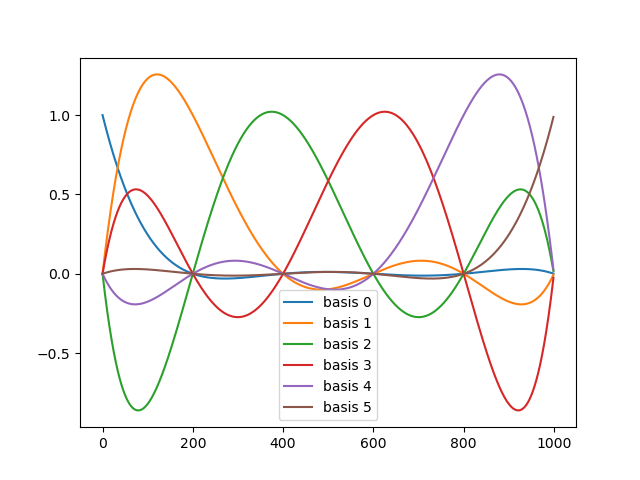
\includegraphics[width=0.75\textwidth]{chapters/element/plots/Lagrange5.png}
\caption{
The basis function of the Lagrange element of order 5. }
\label{fig:Lagrange5}
\end{center}
\end{figure}


The Hermite interpolation generalize the Lagrange interpolation by including also derivative. As such 
the Hermite element is defined in terms of the Hermite interpolation. This is detailed in the following example: 
\begin{exmp}{\textbf{The Hermite element in 1D}.} 
\label{hermite:element}
Let us consider the Hermite interpolation onto $k+1$ points.  
Each point is associated with two degrees of freedom, the function evaluation and the evaluation of the first 
derivative of the function.  
using $m$ derivatives in each point.Hence,  
the number of degrees of freedom, or the number of equations defined by the specification of the nodal 
basis in Definition \ref{nodal:basis} are then $2(k+1)$. As such our polynomial space would be $\mathbb{P}_{2(k+1)}$.    
As such, we may once again compute the nodal basis of the Hermite element. 
Let $H_j$ be the j'th nodal basis, expressed as  
\[ 
H_j = \sum_i \alpha_{ij} x^i 
\]
Then 
where $\alpha_{ij}$ are determined by 
\[ 
d_i(L_j) = L_j(x_i) = \delta_{ij} . 
\]
Here, lets split the degrees of freedom into even and odd numbers, where the even numbering refers to 
point evaluations whereas the odd numbers are the evaluation of the derivatives. 
That is 
\begin{align*} 
d_i(H_j) &= H_j(x_i)  &=  \delta_{ij}, \quad \mbox{ even } i,j   \\
d_i(H_j) &= H'_j(x) |_{x=x_i} &= \delta_{ij}, \quad \mbox{ odd } i,j  
\end{align*}

\end{exmp}

There are a couple of observations that makes the above definite of the finite element really useful 1)   
the mapping between an arbitrary cell of a general mesh and the reference cell can be generalized to 
a mapping between an arbitrary finite element on the mesh and a corresponding reference element and 2)
the degrees of freedom implicitly defines the connectivety of the finite elements in terms of the
connectivity of the underlying cells of the mesh. These observations are detailed below.    

\section{Mapping a reference element onto a physical element. }
Let $x$ and $\hat{x}$ be coordiates in the domains $T$ and $\hat{T}$, respectively, and  
for simplicity we assume an affine mapping between the coordinates:  
\[
x = F_T(\hat{x}) = A_T \hat{x} + x_0   
\]
The Jacobian of the mapping is 
\[
\frac{\partial x}{\partial \hat{x}} = J(\hat{x}) = A_T      
\]
For isoparametric elements, a basis function $\phi$
is the simply defined in terms of its associated function $\hat{\phi}$
on the reference
element, ie. 
\[
\phi(x) = \hat{\phi}(\hat{x}) .  
\]
With this definition we may easily evaluate integrals
\[
\int_T \phi(x) dx = \int_{\hat{T}} \hat{\phi}(\hat{x}) det J d\hat{x},  
\]
and derivatives 
\[
\frac{\partial \phi}{\partial x_i } = \sum_j  \frac{\partial \hat{\phi}}{\partial \hat{x}_j } \frac{\partial \hat{x}_j}{\partial \hat{x}_i } 
\]
As such the finite element engines may perform all the computations on the reference cells, which makes the implementation easy and efficient. 

\section{The connectivity of the mesh and the corresponding finite element space}

The Lagrange element of order 5 was illustrated in Fig.~\cite{fig:Lagrange}. We observe here that the basis function $0$ and $5$ are associated
with the edges $x=0$ and $x=1$, whereas the other functions are all zero at the edges. Hence, the basis function $1, \ldots, 4$ do not connect 
to any other element, whereas the basis $0$ would directly connect to the a corresponding element on the left whereas basis $5$ connects to the 
an element on the right, if present. Hence the edge nodes defines the connectivity and hereby the continuity towards the neighbouring elements. 



\begin{figure}
\begin{center}
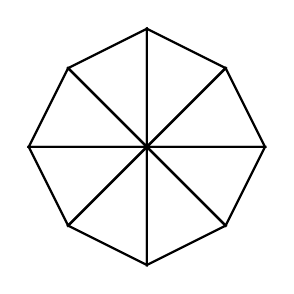
\begin{tikzpicture}
\draw[black, thick] (0,0) -- (1,1) -- (0,1.5) -- cycle;
\draw[black, thick] (0,0) -- (1,1) -- (1.5,0) -- cycle;
\draw[black, thick] (0,0) -- (1,-1) -- (1.5,0) -- cycle;
\draw[black, thick] (0,0) -- (1,-1) -- (0,-1.5) -- cycle;
\draw[black, thick] (0,0) -- (-1,-1) -- (-1.5,0) -- cycle;
\draw[black, thick] (0,0) -- (-1,-1) -- (0,-1.5) -- cycle;
\draw[black, thick] (0,0) -- (-1,1) -- (0,1.5) -- cycle;
\draw[black, thick] (0,0) -- (-1,1) -- (-1.5,0) -- cycle;
\end{tikzpicture}
\caption{
A simple mesh with 8 triangles all meeting at a common point.}
\label{fig:Lagrange5}
\end{center}
\end{figure}




\section{Exercises}
\begin{exercise}
\label{hermite:interval}
Make a Python code that defines a Hermite on the unit interval.       
\end{exercise}



\begin{exercise}
\label{lagrange:triangle}
Make a Python code that defines a Lagrange element of arbitrary order on the reference triangle 
consisting of the vertices $(0,0)$, $(1,0)$ and $(0,1)$. Let $\mathbb{P}_k = \{ x^i y^j \} \mbox{ for } i,j \mbox{ such that } i+j \le k\} $     
\end{exercise}

\begin{exercise}
Check that the interpolation result
of the Bramble-Hilbert lemma \ref{bramblehilbert} applies to the Lagrange interpolation on the unit line. Consider 
for example a function $f = sin(x)$ on the unit interval. The function $f$ is a good example as it cannot be expressed 
as a polynomial of finite order, but can be approximated arbitrary well. 
\end{exercise}

\begin{exercise}
Compute the condition number of the mass matrix when using the Lagrange and the Hermite basis. Compare it with the condition
number when using the basis consisting of monomials, ie. $(1, x, x^2, \ldots)$.   
	The mass matrix on the unit interval  is the matrix $M_{ij} = \int_0^1 \phi_i \phi_j \, dx $ where $\{\phi_i\}$ is 
	the set of basis functions in use. 
\end{exercise}






\chapter{The finite element method for elliptic problems}

\section{The weak formulation and the finite element formulation}

We are now in position to analyze the finite element method
for an elliptic problem in detail and provide rigorous estimates
on the numerical accuracy. We remember the strong formuation:  
Find the solution $u$ of the problem

\begin{eqnarray}
\label{chp3:elliptic}
-\nabla\cdot(k\nabla u)  &=& f \quad \textrm{in}\ \Omega,\\
\label{chp3:Dirichlet}
u&=& g \quad \textrm{on}\ \partial\Omega_D, \\
\label{chp3:Neumann}
k \frac{\partial u}{\partial n}&=& h \quad \textrm{on}\ \partial\Omega_N , 
\end{eqnarray}
where we assume $\partial \Omega = \partial \Omega_D \cup \partial \Omega_N$ 
and $\partial \Omega_D \cap \partial \Omega_N = \emptyset$.

In order to arrive at the weak formulation, we introduce two Sobolev spaces
\begin{align}
H^1_{0, D} (\Omega) &= \{ u \in H^1(\Omega)  | \  T u = 0 \mbox{ on } \partial \Omega_D \}, \\   
H^1_{g, D} (\Omega) &= \{ u \in H^1(\Omega)  | \  T u = g \mbox{ on } \partial \Omega_D \}  .  
\end{align}
Here, both spaces are subspaced of the $H^1$ space introduced in the previous chapter. The 
subspaces include only the functions with appropriate values on the Dirichlet part of the boundary $\partial \Omega_D$.  
As detailed in Chapter \ref{elliptic}, we obtain the weak formulation by 1) multiplying
the equation \eqref{chp3:elliptic} with a test function $v$, 2) employing Gauss-Green's lemma, and 3) employing the 
boundary conditions. 

We arrive at the following \emph{weak formulation}, which includes the precise definitions of spaces of the trial and test functions, source function and boundary conditions: \\
Given $f\in H^{-1}_D(\Omega)$, $h\in H^{-1/2}(\partial \Omega_N)$,  
find $u\in  H^1_{g, D} (\Omega)$ such that  
\begin{equation}
\label{chp3:weak} 
\int_\Omega (k \nabla u) \cdot \nabla v \, dx = \int_\Omega f v \, dx + \int_{\partial \Omega_N} h v \, ds, \quad    \forall v\in  H^1_{0, D} (\Omega).  
\end{equation} 
Here, the negative norms are similar to the negative norms introduced in the previous chapter, although we there had Dirichlet conditions
on the complete boundary. Alternatively, and perhaps simpler from a mathematical point of view is to define it in terms of duality as
in Remark \ref{dualnorm}. When implementing the method, we seldom need to pay attention to what space our source and boundary condition functions reside in, but we remark
that it is sometimes useful to include functions that are not defined in points but only through integration over elements.  

In order to define a finite element method, let $\Omega_h$ be a mesh covering $\Omega$, consisting of a set $E_h$ of cells. 
For simplicity, we assume that the cells are simplices (triangles in 2D, tetrahedrons in 3D). Simplices 
fit very well with standard polynomials, so let ${\cal P}_k$ be the space of 
polynomials of order $k$, i.e., a basis in 2D could be $\{x^i y^{j} \}_{i,j | i+j \le k}$.   
A corresponding finite element method consist of some trial and test spaces 
\begin{align}
V_{h, 0}  &= \{ u \in H^1_{0,D}(\Omega) \ | \  \forall e \in E_h, u|_e \in {\cal P}_k \}, \\   
V_{h, g}  &= \{ u \in H^1_{g,D}(\Omega) \ | \  \forall e \in E_h, u|_e \in {\cal P}_k \} .  
\end{align}
\kent{perhaps instead introduce Lagrange elements} 
The corresponding finite element formulation is then: \\ 
Given $f\in H^{-1}_D$, $h\in H^{-1/2}(\partial \Omega_N)$,  
find $u_h\in  V_{h, g} $ such that  
\begin{equation}
\label{chp3:fem} 
\int_\Omega (k \nabla u_h ) \cdot \nabla v_h \, dx = \int_\Omega f \, v_h \, dx + \int_{\partial \Omega_N} h \, v_h \, ds, \quad    \forall v\in  V_{h, 0} .  
\end{equation} 


\section{What is an elliptic equation ? }

An elliptic partial differential equation is \emph{stricktly positive} with respect to some inner product. 
In order to show that \eqref{chp3:weak} is elliptic, we will need three concepts: Poincare's inequality, lifting, the positivity of $k$. 



Poincare's inequality states that for $u\in  H^1_{0, D}(\Omega)$ we have
\begin{equation} 
\label{poincare}
\|u\|_{L^2(\Omega)}  \le C \| \nabla u\|_{L^2(\Omega)} 
\end{equation} 
We will not prove this inequality in this book (see e.g. ~\cite{evans2022partial}),  
but we note that it can be motivated by considering the Taylor series approximation. 
From basic calculus we know that: 
\[
|f(x+h)|  \le |f(x)| + h \max_{x \le x^* \le x+h } \,  |f'(x^*) | 
\]
Chosing $x$ on $\partial \Omega_D$ makes $f(x)=0$ and hence $f(x+h)$ can be bounded by the derivative
of $f$. Of course, Poincare's result provides a bounds on the integral rather than the pointwise sense 
of Taylor, but the results are similar. 

Lifting, which is often used for theoretical purposes but seldom in implementation, 
refers to changing the problem from having non-homogenous Dirichlet conditions to homogenous Dirichlet conditions.  
Let us assume that $G$ is a function in $H^1(\Omega)$ such that $T u |_{\partial \Omega_D} = g$. 
Clearly, there are infinitely many such functions and in many cases it easy to find such a $G$. 
Then, by linearity, 
$u= u_0 + G$ solves \eqref{chp3:elliptic}--\eqref{chp3:Neumann} with $u_0$ defined as     
\begin{eqnarray}
\label{chp3:elliptic:lift}
-\nabla\cdot(k\nabla u_0 )  &= f +\nabla\cdot(k\nabla G)  &\quad \textrm{in}\ \Omega,\\
\label{chp3:Dirichlet:lift}
u_0&= 0 &\quad \textrm{on}\ \partial\Omega_D, \\
\label{chp3:Neumann:lift}
k \frac{\partial u_0}{\partial n}&= h - k \frac{\partial G}{\partial n} &\quad \textrm{on}\ \partial\Omega_N . 
\end{eqnarray}
Hence, the purpose of the lifting is clear: It transforms a problem with non-homogenous Dirichlet conditions, in which the Poincare's lemma
cannot be applied, to a problem with homogenous Dirichlet conditions where Poincare's lemma can be applied. It is used for theoretical purposes, 
but since $G$ can be choosen arbitrarily as long as it fit the boundary conditions, the procedure do not impose significant constraints on
the analysis. Most analysis therefore only deals with the case of homogenous Dirichlet conditions (see e.g.~\cite{braess2007finite} for more 
detailed coverage). 

In order for \eqref{chp3:elliptic} (or \eqref{chp3:elliptic:lift}) to be an elliptic problem, with  $k(x) \in \mathbb{R}^{d\times d}$ given $\Omega\in \mathbb{R}^d$,  
$k$ needs to be stricktly positive and bounded for all $x\in \Omega$. That is: \\  
For $\forall \xi\in \mathbb{R}^n$ and $\forall x \in \Omega$ there exists a $k_0 > 0$ and $k_1 < \infty$ such that 
\[
	k_0 |\xi|^2  \le    \xi^T k(x) \, \xi \le k_1 |\xi|^2 .   
\]

Given that Poincare's inequality applies and that $k$ is stricktly positive and bounded as defined above, then 
\[
\int_\Omega (k \nabla u) \cdot \nabla v \, dx 
\]
defines an inner product
on $H^1_{0, D} (\Omega)$. 
The result is crucial in this book and is hence left as a series of Exerceises \ref{ex:bilinear}--\ref{ex:poincare3}.  
The exercises show that
\begin{align}
	&\int_\Omega (k \nabla u) \cdot \nabla v \, dx,  \\  
	&\int_\Omega (\nabla u) \cdot \nabla v \, dx,  \\ 
	&\int_\Omega u v + (k \nabla u) \cdot \nabla v \, dx,  \\ 
	&\int_\Omega u v + ( \nabla u) \cdot \nabla v \, dx .  
\end{align}
are all equivalent inner products on $H^1_{0, D}(\Omega)$ . 

\section{An \emph{a priori} Error Estimate}

In the previous chapter we listed some approximation properties of polynomials in general. We will now employ these results in order to
derive \emph{a priori} error estimates. To achieve this we will need that the equation is elliptic and in addition 
the concept of Galerkin orthogonality. 


Inner products are extraordinary useful as they introduce a geometry of the space. For instance, 
a function may be orthogonal to another function. This leads us to our fourth concept: 
Galerkin orthogonality. The concept is simple, let the numerical error be $e_h = u - u_h$. Then we
remark that $v_h \in V_{h,g} \subset H^1_{g, D}$. Hence, letting 
$v=v_h$ in \eqref{chp3:weak} and subtracting \eqref{chp3:fem} we obtain:   
\begin{equation}
\label{chp3:orth}
	\int_\Omega (k \nabla (u -  u_h)) \cdot \nabla v_h \, dx = \int_\Omega (f -f) \, v_h \, dx + \int_{\partial \Omega_N} (h -h)  \, v_h \, ds = 0 \quad    \forall v\in  V_{h, 0} .  
\end{equation}
That is, the numerical error $e_h = u - u_h$ is orthogonal to all test functions $v_h$ used by the finite element method. This is a strong result and
perhaps surprising. The solution $u_h$, found by solving \eqref{chp3:fem} is therefore the best possible solution that can be found in $V_{h, g}$.   

Since, $\int_\Omega (k \nabla u) \cdot \nabla v \, dx$ defines an inner product and associated norm, equivalent with 
the standard $H^1_0$ norm we can employ the approximation result \eqref{bramblehilbert} Chapter \ref{chap-sobolev}. 
The results is called Cea's lemma, and we will later see it in a more general context. 
Here, we briefly prove an error estimate. First, we remark that, as found in the Exercises below  
\[
k_0 \int_\Omega (\nabla u)^2  \, dx \le   \int_\Omega (k \nabla u) \cdot \nabla u \, dx \le   
k_1 \int_\Omega (\nabla u)^2  \, dx,  \\  
\]
As such 
\begin{align*}
	k_0 \int_\Omega (\nabla (u-u_h))^2  \, dx &\le   \int_\Omega (k \nabla (u -u_h)) \cdot \nabla (u-u_h) \, dx \\    
&\le   \int_\Omega (k \nabla (u -u_h)) \cdot \nabla (u-P_m u + P_m u - u_h) \, dx, \\ 
&\le   \int_\Omega (k \nabla (u -u_h)) \cdot \nabla (u-P_m u ) \, dx \\ 
&\le   k_1 \int_\Omega (\nabla (u -u_h)) \cdot \nabla (u-P_m u ) \, dx 
\end{align*}
Here, we use that we may subtract and add $P_m u$ which totals to zero, and remark that both $u_h$ and $P_m u$ 
are in $V_{h,0}$ and hence both are orthogonal to $u - u_h$ as in \eqref{chp3:orth}. 
Further, by using Cauchy-Schartz inequality, which in this case states that   
\begin{align*}
&  \int_\Omega ( \nabla (u -u_h)) \cdot \nabla (u-P_m u ) \, dx \\ \le  
&  
(\int_\Omega ( \nabla (u -u_h))^{2} dx )^{1/2} \,  (\int_\Omega \nabla (u-P_m u )^2 \, dx)^{1/2} 
\end{align*}
we immediately have by the Bramble-Hilbert lemma \eqref{bramblehilbert} that 
\begin{align}
(\int_\Omega ( \nabla (u -u_h))^{2} dx )^{1/2} \le \frac{k_1}{k_0}   (\int_\Omega \nabla (u-P_m u )^2 \, dx)^{1/2} 
 \le \frac{k_1}{k_0}  C h^{m-1} |u|_{m} 
\end{align}


\section{Exercises}

\begin{exercise}
\label{ex:bilinear}
Let $\Omega=(0,1)$.  
Show that 
\[  
a(u, v) = \int_\Omega  u \, v \, dx 
\]
is a bilinear form. 
\end{exercise}

\begin{exercise}
\label{ex:inner}
Let $\Omega=(0,1)$.  
Show that 
\[  
a(u, v) = \int_\Omega  u \, v \, dx 
\]
forms an inner product.  
\end{exercise}




\begin{exercise}
\label{ex:poincare}

Let $\Omega=(0,1)$ then  
for all functions in $H^1_0(\Omega)$ then
Poincar\'e's inequality states that
\[
|u|_{L^2} \le C  |\frac{\partial u}{\partial x}|_{L^2}   
\]
Use this inequality to show that the $H^1$ semi-norm defines 
a norm equivalent with the standard $H^1$ norm on $H^1_0(\Omega)$.  
\end{exercise}



\begin{exercise}
\label{ex:poincare2}

Let $\Omega=(0,1)$.  
Show that 
\[  
a(u, v) = \int_\Omega \nabla u \cdot \nabla v \, dx 
\]
forms an inner product on $H^1_0(\Omega)$  equivalent with the standard
$H^1(\Omega)$ inner product. 
\end{exercise}

\begin{exercise}
\label{ex:poincare3}

Let $\Omega=(0,1)$.  
Show that 
\[  
a(u, v) = \int_\Omega k \nabla u \cdot \nabla v \, dx 
\]
forms an inner product on $H^1_0(\Omega)$ given that $k \in \mathbb{R}^{n \times n}$ is stricktly positive
and bouded. The inner product is equivalent with the $H^1_0(\Omega)$ inner product.  

\begin{exercise}
Make a Python code that defines a Lagrange element of arbitrary order on the reference triangle. 
\end{exercise}

\end{exercise}




\chapter{Discretization of a convection-diffusion problem}

%\long\def\COMMENT#1{\par\vbox{\hrule\vskip1pt \hrule width.125in height0ex #1\vskip1pt\hrule}}


\label{chap-conv}
\section{Introduction}
This chapter concerns convection-diffusion equations of the form: 
\begin{eqnarray*}
-\mu\Delta u + v\cdot \nabla u  &=& f \quad \textrm{in}\ \Omega\\
u&=& g \quad \textrm{on}\ \partial\Omega
\end{eqnarray*}
Here $v$ is  typically a velocity, $\mu$ is the diffusivity,  and $u$ is the 
unknown variable of interest. We assume the Dirichlet condition $u=g$ on 
the boundary, while $f$ is a source term.  

The problem is a singular perturbation problem. That is, the problem is well-posed for $\mu > 0$ but becomes over--determined as $\mu$ tends to zero. For $\mu=0$ the Dirichlet conditions should only be set on the inflow domain $\Gamma$; that is, where $n \cdot v < 0$ for the outward unit normal $n$. 

For many practical situations $\mu>0$, but small in the sense that $\mu \ll |v|$. For such problems, the solution 
will often be similar to the solution of the reduced problem with $\mu=0$ except close to the 
non-inflow boundary $\partial \Omega \backslash \Gamma$. Here, there will typically be a boundary layer $\exp{(\|v\|_\infty x / \mu)}$.      
Furthermore, discretizations often shows unphysical oscillations starting at this boundary layer.    

The next example shows a 1D convection diffusion problem resulting in non-physical oscillations due to the use
of a standard Galerkin approximation. 

\begin{example}{\textbf{Standard Galerkin approximation}} \label{ex1} 
Consider the following 1D problem convection diffusion problem, where $v=-1$ for simplicity: 
\begin{eqnarray}
-u_x - \mu u_{xx} = 0, \\ 
u(0) = 0, u(1) = 1 . 
\end{eqnarray}
The analytical solution is: 
\[
u(x) = \frac{e^{-x/\mu} - 1}{e^{-1/\mu} - 1}. 
\]
Hence, for $\mu \rightarrow 0$ , both $e^{-x/\mu}$ and $e^{-1/\mu}$ 
will be small and $u(x) \approx 1$ unless $x\approx 0$. However, close to the 
outflow boundary at $x=0$, there will be a boundary layer where $u$ has exponential growth. 

We solve the problem with a standard Galerkin method using linear first
order Lagrange elements. To be specific, the variational problem is: \\    
Find $u \in H^1_{(0,1)}$ such that 
\[
\int_0^1 -u_x v + \mu u_x v_x \dx   = 0, \quad \forall v \in H^1_{(0,0)} .  
\]
Here, $H^1_{(0,1)}$ contains functions $u\in H^1$ with $u=0$ at $x=0$ and $u=1$ and $x=1$, while
$H^1_{(0,0)}$ contains functions that are zero both at $x=0$ and $x=1$. We
consider a $\mu=0.01$, a relatively large $\mu$, to enable us to see the
differences on a relatively coarse mesh.     

\begin{figure}
\begin{center}
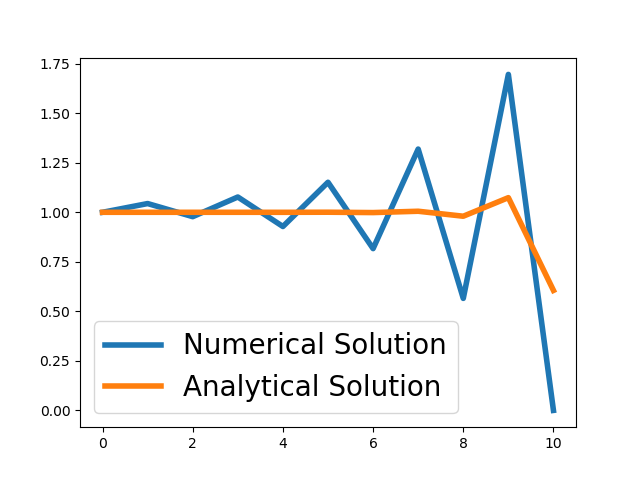
\includegraphics[width=0.45\textwidth]{chapters/conv-diff/plots/conv-diff.png}
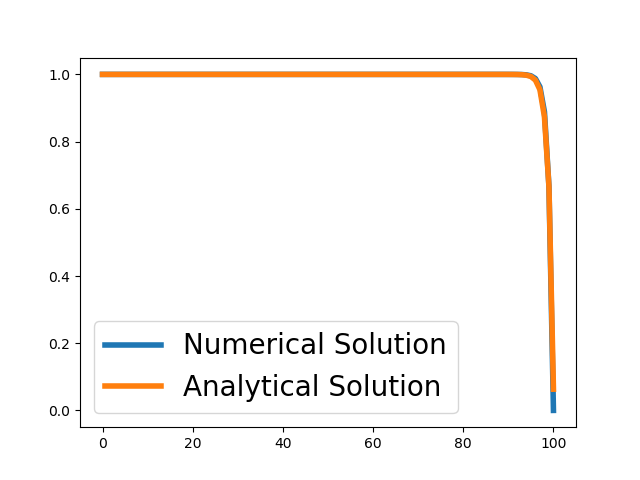
\includegraphics[width=0.45\textwidth]{chapters/conv-diff/plots/conv-diff-hr.png}
\caption{Solution of the convection diffusion problem obtained with 10 and 100 elements. 
The left figure obtained on a mesh with 10 elements shows wild oscillations, while the 
mesh with 100 elements demonstrate a nicely converged solution.}
\label{fig:conv1}
\end{center}
\end{figure}

Both the numerical and analytical solutions are shown in Figure \ref{fig:conv1}. Clearly, 
the numerical solution is polluted by non-physical oscillations on the coarse
mesh with 10 elements, while a good approximation is obtained for 100 elements.     


Finally, we show the complete code for this example: 
\begin{python}
from dolfin import *
for N in [10, 100]:

  mesh = UnitInterval(N)
  V = FunctionSpace(mesh, "CG", 1)

  u = TrialFunction(V)
  v = TestFunction(V)

  mu_value = 1.0e-2 
  mu = Constant(mu_value)
  f = Constant(0)
  h = mesh.hmin()

  a = (-u.dx(0)*v + mu*u.dx(0)*v.dx(0))*dx  
  L = f*v*dx  

  u_analytical = Expression("(exp(-x[0]/e) - 1)/ (exp(-1/%e) - 1)" % (mu_value, mu_value))  
  def boundary(x):
      return x[0] < DOLFIN_EPS or x[0] > 1.0 - DOLFIN_EPS

  bc = DirichletBC(V, u_analytical, boundary) 

  U = Function(V)
  solve(a == L, U, bc) 

  U_analytical = project(u_analytical, V)

  import pylab 
  pylab.plot(U.vector().array())
  pylab.plot(U_analytical.vector().array())
  pylab.legend(["Numerical Solution", "Analytical Solution"])
  pylab.show()
\end{python}
$\square$ 
\end{example}

To understand Example \ref{ex1} we first remark that the discretization corresponds to the following 
central finite difference scheme: 
\begin{eqnarray*}
-\frac{\mu}{h^2}\left[u_{i+1}-2u_i+u_{i-1}\right] - 
\frac{v}{2h}\left[u_{i+1}-u_{i-1}\right] &=& 0, \quad i=1,\ldots,N-1\\
u_0=0,\quad u_N=1 &&
\end{eqnarray*}
Above, we kept $v$ as a variable such that we may discuss the directionality of upwinding in terms of the convection. 
Clearly, if $\mu=0$ then the scheme reduces to  
\begin{eqnarray*}
-\frac{v}{2h}\left[u_{i+1}-u_{i-1}\right] &=& 0, \quad i=1,\ldots,N-1\\
u_0=0,\quad u_N=1 &&
\end{eqnarray*}
Here, it is clear that $u_{i+1}$ is coupled to $u_{i-1}$, but not to 
$u_{i}$. 
Hence, this scheme allow for an alternating
sequence of $u_{i+1}=u_{i-1}=\ldots$, while $u_{i}=u_{i-2}=\ldots$
resulting in oscillations. 

One cure for these oscillations is upwinding. That is, instead
of using a central difference scheme, we employ the following difference
scheme:   
\begin{eqnarray*}
\frac{du}{dx} (x_i) = \frac{1}{h}[u_{i+1}-u_{i}] \quad   \mbox{ if } \ v < 0, \\ 
\frac{du}{dx} (x_i) = \frac{1}{h}[u_{i}-u_{i-1}] \quad  \mbox{ if } \ v > 0 .  
\end{eqnarray*}
Using this scheme, oscillations will disappear. The approximation will however only be first order.

There is a relationship between upwinding and artificial diffusion.  If we discretize $u_x$ with a central difference and add diffusion as $\epsilon =h/2 \Delta $ we get
\begin{eqnarray*}
 \frac{u_{i+1}  -  u_{i-1}}{2 h}    &  \textrm{central scheme, first order derivative}  \\
+ \frac{h}{2} \, \frac{-u_{i+1}   + 2 u_{i}    -u_{i-1}}{h^2}  &  \textrm{central scheme, second order derivate}   \\
= \frac{u_{i} -u_{i-1}}{h} &  \textrm{upwind scheme}   
\end{eqnarray*}

\noindent
Hence, upwinding is equivalent to adding artificial diffusion with $\epsilon=h/2$; that is, in both cases we actually solve the problem
\[-(\mu+\epsilon)u_{xx} + vu_x = f.\]
using a central difference scheme. 

Finite difference upwinding is difficult to express using finite elements methods, but
it is closely to adding some kind of diffusion to the scheme.  
The next example shows the solution of the problem in Example \ref{ex1} with 
artificial diffusion added. 

\begin{example}{\textbf{Stabilization using artificial diffusion}} \label{cd:ex2} 
Consider again the following 1D problem convection diffusion problem: 
\begin{eqnarray}
-u_x - \mu u_{xx} = 0, \\ 
u(0) = 0, u(1) = 1 . 
\end{eqnarray}

We solve the problem with a standard Galerkin method using linear first
order Lagrange elements as before, but we add artificial diffusion. To be specific, the variational problem is:  \\   
Find $u \in H^1_{(0,1)}$ such that 
\[
\int_0^1 -u_x v + (\mu + \beta h) u_x v_x = 0, \quad \forall v \in H^1_{(0,0)},    
\]
where $\beta=0.5$ corresponds to the finite difference scheme with artificial diffusion mentioned
above.  Below is the code for the changed variational form:

\begin{python}
  beta_value = 0.5 
  beta = Constant(beta_value)
  f = Constant(0)
  h = mesh.hmin()
  a = (-u.dx(0)*v + mu*u.dx(0)*v.dx(0) + beta*h*u.dx(0)*v.dx(0))*dx  
\end{python}

\begin{figure}
\begin{center}
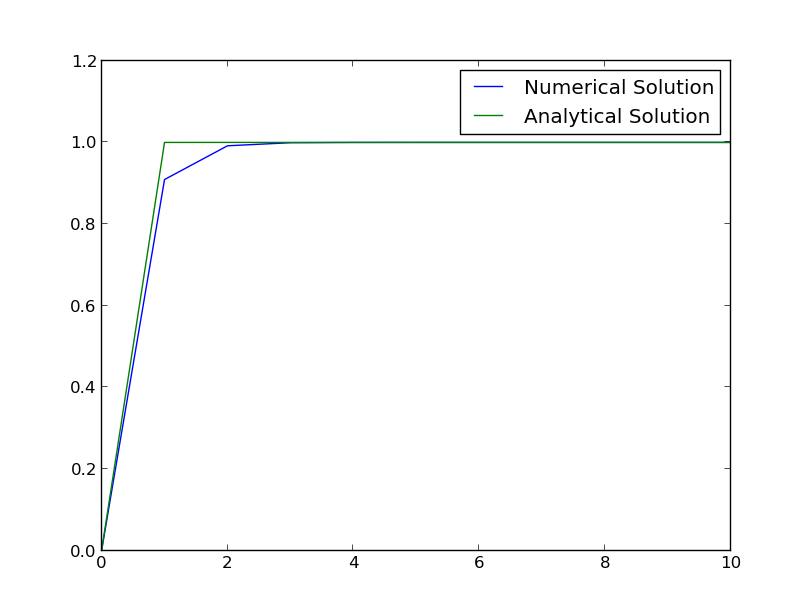
\includegraphics[width=0.45\textwidth]{chapters/conv-diff/plots/conv-diff-stab.png}
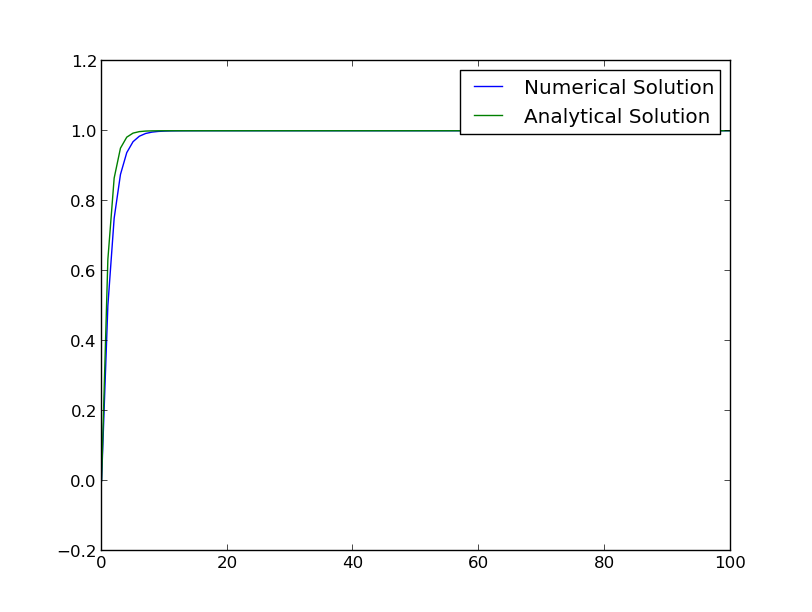
\includegraphics[width=0.45\textwidth]{chapters/conv-diff/plots/conv-diff-hr-stab.png}
\caption{Solution of the convection diffusion problem obtained with 10 and 100 elements
using artificial diffusion to stabilize.}
\label{fig:conv2}
\end{center}
\end{figure}

Figure \ref{fig:conv2} shows the solution for 10 and 100 elements when using artificial diffusion 
stabilization.  Clearly, the solution for the coarse grid has improved dramatically since the
oscillations have vanished and the solution appear smooth. It is, however, interesting to note
that the solution for the fine mesh is actually less accurate than the solution in Fig \ref{fig:conv2} 
for the corresponding fine mesh. The reason is that the scheme is now first order, while the 
scheme in Example \ref{ex1} is second order.    
\end{example}



\section{Streamline diffusion/Petrov-Galerkin methods}
In the previous section we saw that artificial diffusion may be added to convection diffusion dominated problems to avoid 
oscillations. The diffusion was, however, added in a rather ad-hoc manner.  
Here, we will see how diffusion may be added in a consistent way; 
that is, without changing the solution as $h\rightarrow 0$. 
This leads us to streamline diffusion using the Petrov-Galerkin method.
Our problem reads: \\ 
Find $u$ such that 
\begin{eqnarray*}
-\mu\Delta u + v\cdot\nabla u &=& f \quad \textrm{in}\ \Omega, \\
u&=& g \quad \textrm{on}\ \partial\Omega .
\end{eqnarray*}
The \textbf{weak formulation} reads: \\
Find $u\in H_g^1$ such that 
\[
a(u,w) = b(w) \quad \forall\ w\in H_0^1, 
\]
where
\begin{eqnarray*}
a(u,w) &=& \int_\Omega\mu\nabla u \cdot \nabla w \dx + \int_\Omega v \cdot \nabla uw \dx,   \\
b(w) &=& \int_\Omega fw \dx . 
\end{eqnarray*}
Here, $H_g^1$ is the subspace of $H^1$ where the trace equals $g$ on the boundary $\partial \Omega$.  

The \textit{standard Galerkin} discretization is: \\
Find $u_h\in V_{h,g}$ such that 
\begin{equation}
\label{Galerkin}
a(u_h, v_h) = (f,v_h)\ \forall v_h\in V_{h,0}.
\end{equation}
Here, $V_{h,g}$  and $V_{h,0}$ are the subspaces with traces that equals $g$ and $0$ on 
the boundary, respectively.  

Adding artificial diffusion 
to the standard Galerkin discretization, 
as was done in Example \ref{cd:ex2}, 
can be done as: \\ 
Find $u_h\in V_{h,g}$ such that 
\[
a(u_h, v_h) + \frac{h}{2}(\nabla u_h, \nabla v_h)  = (f,v_h)\ \forall v_h\in V_{h,0}.
\]
Let
\[
\tau(u, v_h) =  a(u_h, v_h) - (f,v_h). 
\]
Then the \emph{truncation error} is first order in $h$; that is, 
\[
\tau(u) = \sup_{v \in V_h, v \not = 0} \frac{\tau (u, v_h)}{\|v\|_{V}} \sim \mathcal{O}(h). 
\]
Hence, the scheme is \emph{consistent} in the sense that 
\[
\lim_{h\rightarrow 0} \tau (u) \rightarrow 0 .  
\]
However, it is not \emph{strongly consistent} in the sense that $\tau(u) = 0$ for every
discretization, which is what is obtained with the Galerkin method due
to Galerkin-orthogonality:   
\[
\tau(u, v_h) =  a(u_h, v_h) - (f,v_h) = a(u_h - h, v_h) = 0 \quad \forall v_h \in V_h. 
\]


The \textit{Streamline diffusion/Petrov-Galerkin} method introduces a strongly consistent  
diffusion by employing alternative test functions. Let us therefore
assume that we have a space of test functions $W_h$.   
Abstractly, the Petrov-Galerkin method appears very similar to the Galerkin method, that is: \\ 
Find $u_h\in V_{h,g}$ such that 
\[
a(u_h, v_h) = (f,v_h) \quad \forall v_h\in W_{h,0}.
\]
Again, $V_{h,g}$  and $W_{h,0}$ are the subspaces with traces that equals $g$ and $0$ on 
the boundary, respectively.  
Notice that the only difference from the standard Galerkin formulation is that test and trial functions differ. 

On matrix form, the standard Galerkin formulation reads: 
\begin{equation}
A_{ij} = a(N_i, N_j ) = \int_\Omega\mu\nabla N_i \cdot \nabla N_j \dx + \int_\Omega v \cdot \nabla N_iN_j \dx, 
\label{eq:wGalerkin_A}
\end{equation}
while for the Petrov Galerkin method, we use the test functions $L_j$: 
\[A_{ij} = a(N_i, L_j ) = \int_\Omega\mu\nabla N_i \cdot \nabla L_j \dx + \int_\Omega v \cdot \nabla N_iL_j \dx\]
A clever choice of $L_j$ will enable us to add diffusion in a consistent way. To make sure
that the matrix is still quadratic, we should however make sure that the dimension of 
$V_h$ and $W_h$ are equal. 

Let $L_j$ be defined as $L_j = N_j + \beta h \, v\cdot\nabla N_j$. Writing out the matrix $A_{ij}$ in \eqref{eq:wGalerkin_A} now gives
\begin{eqnarray*}
A_{ij} &=& a(N_i, N_j + \beta h \, v\cdot\nabla N_j )\\
&=& \int_\Omega\mu\nabla N_i\cdot\nabla (N_j + \beta h \,  v\cdot\nabla N_j) \dx + \int_\Omega v \cdot \nabla N_i\cdot (N_j + \beta h \, v\cdot\nabla N_j) \dx\\
&=&\underbrace{
\int_\Omega\mu\nabla N_i \cdot \nabla N_j \dx + \int_\Omega v \cdot \nabla N_i\, N_j \dx}_
{\textrm{standard Galerkin}}
\\
&&\lefteqn{
+\underbrace{
\beta h \, \int_\Omega\mu\nabla N_i\cdot\nabla(v \cdot \nabla N_j) \dx
}_
{=0\ \textrm{third order term,  for linear elements}}+
\underbrace{\beta h \, \int_\Omega (v\cdot\nabla N_i) (v\cdot\nabla N_j) \dx}
_{\textrm{Artificial diffusion in $v$ direction}}
}
\end{eqnarray*}

Notice that also the righthand side changes
\[b(L_j) = \int_\Omega fL_j \dx = \int_\Omega f(N_j + \beta h \, v\cdot\nabla N_j) \dx\]
Thus, both the matrix and the righthand side are changed such that artificial diffusion is added in a consistent way. 

We summarize this derivation by stating the SUPG problem. 
Find $u_{h,sd}\in H_g^1$ such that 
\begin{equation}
\label{SUPG} 
a_{sd} (u,w) = b_{sd}(w) \quad \forall w\in H_0^1, 
\end{equation}
where
\begin{eqnarray*}
a_{sd}(u,w) &=& \int_\Omega\mu\nabla u \cdot \nabla w \dx + \int_\Omega v \cdot \nabla uw \dx \\
            &+& \beta h \,  \int_\Omega (v\cdot\nabla u) (v\cdot \nabla w) \dx  + \beta h \,  \mu \sum_e \int_{\Omega_e} -\Delta u (v\cdot\nabla w) \dx ,  \\
b_{sd} (w) &=& \int_\Omega fw \dx + \beta h \, \int_\Omega f v \cdot \nabla w \dx . 
\end{eqnarray*}



\section{Well posedness of the continuous problem}
Before we discuss error estimates of the discrete problem, we
briefly describe the properties of the continuous problem. 

\begin{theorem}{\textbf{Lax-Milgram theorem}} \\
Let $V$ be a Hilbert space, $a(\cdot, \cdot)$ be 
a bilinear form, $L(\cdot)$ a linear form, and let the following three conditions be satisfied: 
\begin{enumerate}
\item $a(u,u) \ge \alpha \|u\|^2_V, \quad \forall u \in V$,  \label{LM1} 
\item $a(u,v) \le C \|u\|_V \|v\|_V, \quad \forall u, v \in V$,  \label{LM2} 
\item $L(v) \le D \| v \|_V, \quad \forall v \in V$ .  \label{LM3} 
\end{enumerate}
Then the problem: Find $u\in V$ such that 
\[
a(u,v) = L(v) \quad \forall v \in V. 
\]
is well-posed in the sense that there exists a unique solution with the following 
stability condition
\[
\|u \|_V \le \frac{C}{\alpha} \|L\|_{V^*} .  
\]
\end{theorem}
Condition \eqref{LM1} is often refereed to as coersivity or positivity, while
\eqref{LM2} is called continuity or boundedness. Condition \ref{LM3} simply
states that the right-hand side should be in the dual space of $V$.    

In the following we will use Lax-Milgram's theorem to show that the convection-diffusion problem is well-posed. 
The Lax-Milgram's theorem is well-suited since it does not require symmetry of the bilinear form. 


We will only consider the homogeneous Dirichlet conditions in the current 
argument\footnote{Has the argument for reducing non-homogeneous Dirichlet conditions
to homogeneous Dirichlet conditions been demonstrated elsewhere?}.   
From Poincare's lemma we know  that 
\[
\|u\|_0 \le C_\Omega |u|_1.  
\]
Using Poincare, it is straightforward to show that the 
semi-norm     
\[
|u|_1 = (\int (\nabla u)^2   \dx)^{1/2}  
\]
and the standard $H^1$ norm 
\[
\|u \|_1  = (\int (\nabla u)^2 + u^2  \dx)^{1/2}  
\]
are equivalent. Hence, on $H^1_0$ the $|\cdot|_1$ is a norm
equivalent the $H^1$-norm. Furthermore, this norm will be easier to 
use for our purposes.  

For the convection-diffusion problem, we will consider two cases 1) incompressible flow, where
$\nabla \cdot v = 0 $ and 2) compressible flow, where $\nabla \cdot v \not = 0 $.  
Let us for the begin with the incompressible case.  
Further, let 
\begin{eqnarray*}
b(u,w) &=& \int_\Omega\mu\nabla u\nabla w \dx\\
c_v(u,w) &=& \int_\Omega v \cdot \nabla u \,w \dx\\
a(u,w) &=& a(u,w) + b(u,w)\\
\end{eqnarray*}
Furthermore, assuming for the moment that $u \in H^1_g, w\in H^1_0$, we have  
\begin{eqnarray*}
c_v(u,w) &=& \int_\Omega v\cdot \nabla u\, w \dx  \\ 
         &=&-\int_\Omega v\cdot \nabla w \, u \dx 
- \underbrace{\int_\Omega \nabla \cdot v \, u \, w \dx}_{= 0 \textrm{ (incompressibility)}} 
+ \underbrace{\int_\Gamma u \, w \, v \cdot n}_{ = 0  \textrm{ (Dirichlet conditions)}} \\       
         &=& - c_v(w,u) . 
\end{eqnarray*}
and therefore $c_v(\cdot, \cdot)$ is skew-symmetric. Letting $w=u$ we obtain that   
$c_v(u,u) = -c_v(u,u)$, which means that $c_v(u,u)=0$. 
Therefore, the first condition in Lax-Milgram's theorem \eqref{LM1} is satisfied:   
\[  
a(u,u) = b(u,u) \ge \mu |u|_1^2 .  
\]

The second condition, the boundedness of $a$ \eqref{LM2}, follows by applying Cauchy-Schwartz inequality
if we assume bounded flow velocities $\|v\|_{\infty}$.  
\begin{eqnarray*}
a(u,v) &=& \int_\Omega\mu\nabla u\nabla w \dx + \int_\Omega v\nabla uw \dx\\
       &\le& \mu |u|_1 |w|_1  + \|v\|_{\infty} |u|_1 \|w\|_0 \\   
       &\le& (\mu + \|v\|_{\infty} C_\Omega )  |u|_1 |v|_1 .    
\end{eqnarray*}

The third condition simply means that the right-hand side needs to be in the dual 
space of $H^1_g$. Hence, we obtain the following bounds by Lax-Milgram's theorem:   
\[
|u|_1 \le \frac{ \mu + C_\Omega \|v\|_{\infty}}{\mu} \|f\|_{-1} . 
\]
Notice that for convection-dominated problems $ C_\Omega \|v\|_{\infty} \gg \mu$ 
and the stability constant will therefore be large. 

In the case where $\nabla \cdot v \not = 0$, we generally obtain that $c_v(u,u) \not = 0$. 
To ensure that $a(u,u)$ is still positive, we must then put some restrictions on 
the flow velocities. That is, we need    
\[
|c_v(u,u)| \le a(u,u) .  
\]
If $C_\Omega \|v\|_\infty \le D \mu$ with $D < 1$ we obtain   
\begin{eqnarray*}
a(u,u) &=& \int_\Omega\mu\nabla u\nabla u \dx + \int_\Omega v\nabla uu \dx\\
       &\ge & \mu |u|_1 |v|_1  - \|v\|_{\infty} |u|_1 \|u\|_0 \\   
       &\ge& (\mu - \|v\|_{\infty} C_\Omega )  |u|_1 |u|_1 \\    
       &\ge& (\mu (1-D))  |u|_1^2 .    
\end{eqnarray*}
Further, the second condition of Lax-Milgram's theorem still applies.   
However, that $C_\Omega \|v\|_\infty \le D \mu$ is clearly very restrictive 
compared to the incompressible case.   

We remark that the Lax-Milgram conditions in the presence of the SUPG clearly will not 
be satisified in the continuous case because of the third order term
$ -\Delta u (v\cdot\nabla w)$. With this term, the second condition of Lax-Milgram is not satisified
with $C \le \infty$.  

Finally, in order to make the  
term $c_v(u,u)$ skew-symmetric, it was required that 
the boundary integral $\int_\Gamma u^2 \, w  \cdot n $ was zero.  
This was a consequence of the Dirichlet conditions. 
 In general, this is neither needed nor possible
at Neumann boundaries. As long as $\int_\Gamma u^2 \, w \cdot n \ge 0 $, the above argumentation is valid. From a 
physical point of view this means that there is outflow at the Neumann boundary, i.e., that $w\cdot n \ge 0$.  

\section{Error estimates}

Finally, we provide some error estimates for the
Galerkin method and the SUPG method applied to the
convection-diffusion equation. Central in the derivation
of both results are the following interpolation result.   


\begin{theorem}{\textbf{Approximation by interpolation}}\\
There exists an interpolation operator $I_h: H^{t+1} \rightarrow V_h$ 
where $V_h$ is a piecewise polynomial field of order $t$ with the property that   
for any $u\in H^t(\Omega)$ 
\[
\| u - I_h u \|_m \le  B h^{t+1-m} \|u\|_{t+1}  .  
\]
\end{theorem}
\begin{proof} %FIXME, this dose not look good
The bounds on the interpolation error is provided by 
the Bramble-Hilbert lemma for $t\ge 1$  and Clement's result (the case $t=1$), 
cf. e.g.~\cite{braess2007finite, brenner2008mathematical}.  
\end{proof}

For the Galerkin method the general and elegant result of Cea's lemma
provide us with error estimates. Cea's lemma applies to general 
conforming approximations, i.e. when $V_h \subset V$. In our
case $V=H_0^1(\Omega)$ and $V_h$ is a finite element subspace such 
as for example  a discretization in terms of the Lagrange elements (of any order). Hence, in our case 
$\|\cdot\|_V= |\cdot|_1$ and the $H^1$ semi-norm is equivalent with the full 
$H^1$ norm due to Poincare's inequality. 

\begin{theorem}{\textbf{Cea's lemma}} \\
Suppose the conditions for Lax-Milgram's theorem is satisfied and that
we solve the linear problem \eqref{Galerkin} on a finite element space
of order $t$. Then,     
\[
\|u-u_h\|_V     \le C_1 \frac{C B}{\alpha}  h^{t} \|u\|_{t+1}.   
\]
Here $C_1 = \frac{C B}{\alpha}$, where $B$ comes from the approximation property 
and $\alpha$ and $C$ are the constants of Lax-Milgram's theorem.    
\end{theorem}

\begin{proof}
The proof is straightforward and follows from the Galerkin orthogonality: 
\[
a(u - u_h, v) = 0, \quad \forall v \in V_h 
\]
Since $V_h \subset V$: 
\begin{eqnarray*}
\alpha \|u-u_h\|^2_{V} &\le& a(u-u_h, u-u_h)    \\ 
 &=& a(u-u_h, u-v) - a(u-u_h, v-u_h) \\ 
 &\le& C \|u-u_h\|_V \| u-v\|_V  .      
\end{eqnarray*}
Since $v-u_h\in V_h$. Furthermore,  $v$ is arbitrary and we may therefore choose $v = I_h u$ and obtain:  
\[
	|u-u_h|_1 \le \frac{C}{\alpha} |u - I_h u|_1 \le  \frac{CB}{\alpha} h^{t} \|u\|_t,   
\]
where $t-1$ is the order of the polynomials of the finite elements. 
\end{proof}

We remark, as mentioned above, that 
$\frac{C}{\alpha}$ is large for convection dominated problems and that this is what
causes the poor approximation on the coarse grid, shown in Example \ref{ex1}.  


To obtain improved error estimates for the SUPG method, we introduce  
an alternative norm: 
\begin{equation}
\label{supg:norm}
\|u\|_{sd} = \left(h\|v\cdot\nabla u\|^2 +  \mu |\nabla u|^2\right)^{1/2}
\end{equation}


\begin{theorem}
Suppose the conditions for Lax-Milgram's theorem is satisfied 
in the Hilbert space defined by the SUPG norm \eqref{supg:norm}
and that
we solve the SUPG problem \eqref{SUPG} on a finite element space
of order $1$. Then,  
\[\|u-u_h\|_{sd} \le Ch^{3/2}\|u\|_{2}\]
\end{theorem}

\begin{proof}
The proof can be found in e.g. \cite{elman2014finite, quarteroni2008numerical}. 
\end{proof}

\section{Exercises}

\begin{exercise}
Show that the matrix obtained from a central difference scheme applied to 
the operator $L u = u_x$ is skew-symmetric. Furthermore, show that
the matrix obtained by linear continuous Lagrange elements are also 
skew-symmetric. Remark: The matrix is only skew-symmetric in the  interior
of the domain, not at the boundary.    
\end{exercise}

\begin{exercise}
Estimate numerically the constant in Cea's lemma for various $\alpha$ and $h$ for the  Example \ref{ex1}. 
\end{exercise}

\begin{exercise}
Implement the problem $u=sin(\pi x)$, and $f = -\alpha u_{xx} - u_x$ and 
estimate numerically the constant in Cea's lemma for various $\alpha $.       
Compare with the corresponding constant estimated from Example \ref{ex1}. 
\end{exercise}


\begin{exercise}
Implement the problem $u=sin(\pi x)$, and $f = -\alpha u_{xx} - u_x$ using
SUPG and estimate the constants in the error estimate obtained by 
both the $|\cdot|_1$ and  the $\| \cdot \|_{v}$      
norms. 
Compare with the corresponding constant estimated from Example \ref{ex1}. 
\end{exercise}

 
 
\begin{exercise}
Investigate whether the coersivity condition holds when a 
homogeneous Neumann condition is assumed on the outflow. 
You may assume that $v\cdot n > 0$.   
\end{exercise}

\begin{exercise}
Consider the eigenvalues of the operators, 
$L_1$, $L_2$, and $L_3$, where
$L_1 u = u_x$, $L_2 u = -\alpha u_{xx}$, $\alpha=1.0e^{-5}$, 
and $L_3 = L_1 + L_2$, with homogeneous Dirchlet conditions. 
For which of the operators are the eigenvalues positive and
real? Repeat the exercise with $L_1 = x u_x$.   
\end{exercise}


\begin{exercise}
Compute the Soblev norms $\|\cdot\|_m$ of the function $sin(k \pi x)$ on 
the unit interval. Assume that the Soblev norm is $\|u\|_m = (-\Delta^m u, u)^{1/2}$.     
What happens with negative $m$? You may use either Fourier transformation or 
compute (eigenvalues of) powers of the stiffness matrix. 
\end{exercise}

\begin{exercise}
Perform numerical experiments to determine the order of approximation with respect 
to various Soblev norms and polynomial orders for the function  
$sin(k \pi x)$ on 
the unit interval.
\end{exercise}






%\section{Further reading}
%Further discussions on the convection-diffusion equation can be 
%found in, e.g.,\cite{elman2005finite, johnson2009numerical, quarteroni2008numerical}.  



\chapter{Stokes problem}
\label{chap-stokes}
%\long\def\COMMENT#1{\par\vbox{\hrule\vskip1pt \hrule width.125in height0ex #1\vskip1pt\hrule}}

%\newcommand{\norm}[1]{ |\!|\!| #1 |\!|\!|}
%\newtheorem{theorem}{Theorem}[section]
%\newtheorem{example}{Example}[section]
%\newtheorem{exercise}{Exercise}[section]
%\newtheorem{exercise}{Exercise}[chapter]
%\newtheorem{remark}{Remark}[section]
%\newtheorem{proof}{Proof}[section]


\section{Introduction}
The Stokes problem describes the flow of a slowly moving viscous incompressible Newtonian
fluid.  Let the fluid domain be denoted $\Omega$. We assume that $\Omega$ is a bounded domain in $\mathbb{R}^n$ with a smooth boundary. Furthermore, let $u : \Omega \rightarrow \mathbb{R}^n$ be
the fluid velocity and $p:\Omega \rightarrow \mathbb{R}$ be the fluid pressure.
The strong form of the Stokes problem can then be written as
\begin{eqnarray}
-\Delta u + \nabla p &=& f, \mbox{ in } \Omega,   \\
\nabla \cdot u &=& 0, \mbox{ in } \Omega, \\
u &=& g, \mbox{ on } \partial \Omega_D, \\
\frac{\partial u}{\partial n} - p n  &=& h, \mbox{ on } \partial \Omega_N.
\end{eqnarray}
Here, $f$ is the body force, $\partial \Omega_D$ is the Dirichlet
boundary, while $\partial \Omega_N$ is the Neumann
boundary. Furthermore, $g$ is the prescribed fluid velocity on the
Dirichlet boundary, and $h$ is the surface force or stress on the
Neumann boundary. These boundary condition leads to a well-posed
problem provided that neither the Dirichlet nor Neumann boundaries are
empty.  In case of only Dirichlet conditions the pressure is only
determined up to a constant, while only Neumann conditions leads to
the velocity only being determined up to a constant.

These equations are simplifications of the Navier--Stokes equations for
very slowly moving flow.  In contrast to elliptic equations, many
discretizations of this problem will lead to instabilities.  These
instabilities are particularly visible as non-physical oscillations in
the pressure. The following example illustrate such oscillations.

\begin{example}{Poiseuille flow} \\
One of the most common examples of flow problems that can be solved
analytically is Poiseuille flow. It describes flow in a straight
channel (or cylinder in 3D).  The analytical solution is $u=(y\,
(1-y), 0)$ and $p = 1-x$.  Since the solution is know, this flow
problem is particularly useful for verifying that the code or
numerical method. We therefore begin by discretizing the problem in
the simplest way possible; that is, linear continuous/Lagrange elements
for both velocity and pressure. The results is shown Figure
\ref{fig:stokes1}. Clearly, the velocity is approximated satisfactory,
but the pressure oscillate widely and is nowhere near the actual
solution.
\begin{figure}
\begin{center}
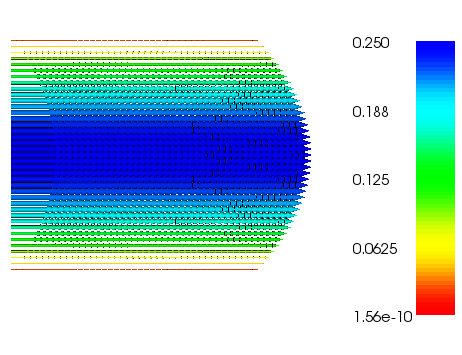
\includegraphics[width=0.45\textwidth]{chapters/Stokes_problem/plots/stokes_velocity.png}
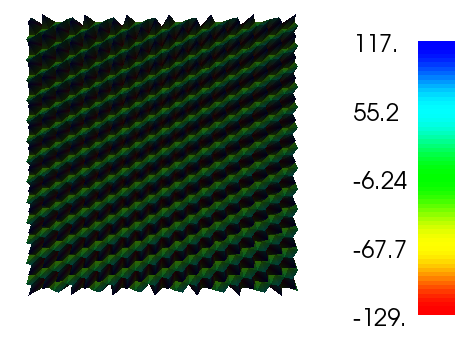
\includegraphics[width=0.45\textwidth]{chapters/Stokes_problem/plots/stokes_pressure_instabilities.png}
\caption{Poiseuille flow solution obtained with linear continuous elements for
both velocity and pressure. The left figure shows the (well-represented) velocity while the right shows
the pressure (with the wild oscillations).}
\label{fig:stokes1}
\end{center}
\end{figure}

% inf56xx-2013/code/stokes/stokes_p1p1.py
\begin{python}
from dolfin import *

def u_boundary(x):
  return x[0] < DOLFIN_EPS or x[1] > 1.0 - DOLFIN_EPS or x[1] < DOLFIN_EPS

def p_boundary(x):
  return  x[0] > 1.0 - DOLFIN_EPS

mesh = UnitSquare(40,40)
V = VectorFunctionSpace(mesh, "Lagrange", 1)
Q = FunctionSpace(mesh, "Lagrange", 1)
#Q = FunctionSpace(mesh, "DG", 0)
W = MixedFunctionSpace([V, Q])

u, p = TrialFunctions(W)
v, q = TestFunctions(W)

f = Constant([0,0])

u_analytical = Expression(["x[1]*(1-x[1])", "0.0"])
p_analytical = Expression("-2+2*x[0]")

bc_u = DirichletBC(W.sub(0), u_analytical, u_boundary)
bc = [bc_u]

a = inner(grad(u), grad(v))*dx + div(u)*q*dx + div(v)*p*dx
L = inner(f, v)*dx

UP = Function(W)
A, b = assemble_system(a, L, bc)
solve(A, UP.vector(), b, "lu")

U, P = UP.split()

plot(U, title="Numerical velocity")
plot(P, title="Numerical pressure")

U_analytical = project(u_analytical, V)
P_analytical = project(p_analytical, Q)

plot(U_analytical, title="Analytical velocity")
plot(P_analytical, title="Analytical pressure")

interactive()
\end{python}



However, when using the second order continuous elements for the velocity and
first order continuous elements for the pressure, we obtain the perfect solution
shown in Figure \ref{fig:stokes2}.
\begin{figure}
\begin{center}
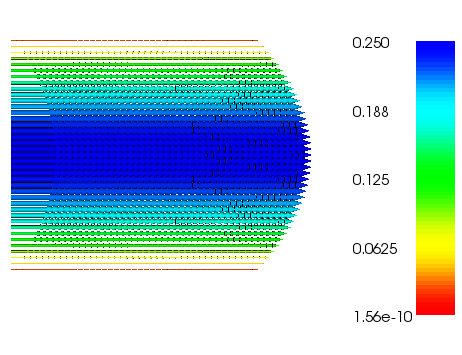
\includegraphics[width=0.45\textwidth]{chapters/Stokes_problem/plots/stokes_velocity.png}
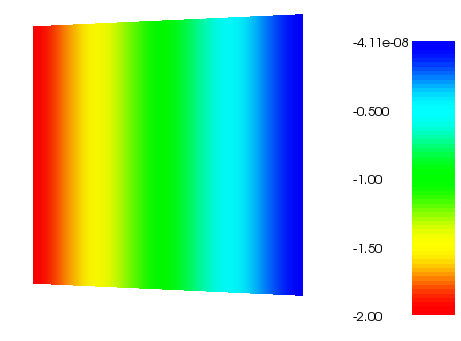
\includegraphics[width=0.45\textwidth]{chapters/Stokes_problem/plots/stokes_pressure.png}
\caption{Poiseuille flow solution obtained with quadratic continuous elements for the
velocity and linear continuous elements for the pressure. The left figure shows the velocity while the right shows
the pressure. Both the velocity and the pressure are correct.}
\label{fig:stokes2}
\end{center}
\end{figure}
\end{example}

The previous example demonstrates that discretizations of the Stokes problem may lead
to, in particular, strange instabilities in the pressure. In this chapter we will describe why this
happens and several strategies to circumvent this behaviour.

\section{Finite Element formulation}

Let us first start with a weak formulation of Stokes problem:
Find $u\in H^1_{D,g}$ and $p\in L^2$.
\begin{eqnarray*}
a(u,v) + b(p,v) &=& f(v), \quad v\in H_{D,0}^1\\
b(q,u) &=& 0,\quad q\in L^2,
\end{eqnarray*}
where
\begin{eqnarray*}
a(u,v) &=& \int\nabla u : \nabla v \dx, \\
b(p,v) &=& \int p \, \nabla \cdot v \dx, \\
f(v) &=& \int f\, v \dx + \int_{\Omega_N} h \, v \, \ds  .
\end{eqnarray*}
Here
$H^1_{D,g}$ contains functions  in $H^1$ with trace $g$ on $\partial \Omega_D$.
To obtain symmetry we have substituted $\hat{p} = - p$ for the pressure
and is referint to $\hat{p}$ as p.

As before the standard finite element formulation follows directly from the weak formulation:
Find $u_h\in V_{g,h}$ and $p_h\in Q_h$ such that
\begin{eqnarray}
\label{eq:stdGalerkin1}
a(u_h, v_h ) + b(p_h, v_h) &=& f(v_h),\quad \forall v_h\in V_{0,h}, \\
\label{eq:stdGalerkin2}
b(q_h, u_h) &=& 0,\quad \forall q_h \in Q_h .
\end{eqnarray}
Letting $u_h=\sum_{i=1}^n u_i N_i$, $p_h=\sum_{i=1}^m p_i L_i$, $v_h=N_j$, and $q_h=L_j$
we obtain a linear system on the form
\begin{equation}
\left[ %matrix
	\begin{array}{cc}
	A & B^T\\
	B & 0
	\end{array}
\right]
\left[ %vector
	\begin{array}{c}
	u\\
	p
	\end{array}
\right]
=
\left[ %vector
	\begin{array}{c}
	f\\
	0
	\end{array}
\right]
\label{la:stokes}
\end{equation}
Here
\begin{eqnarray}
A_{ij} = a(N_i,N_j) &=& \int\nabla N_i \nabla N_j \dx, \\
B_{ij} = b(L_i,N_j) &=& \int\nabla L_i \, N_j \dx.
\end{eqnarray}
Hence, $A$ is $n\times n$, while $B$ is $m\times n$,
where $n$ is the number of degrees of freedom for the velocity field, while
$m$ is the number of degrees of freedom for the pressure.



Is the system \eqref{la:stokes} invertible?  For the moment, we assume that the submatrix $A$ is invertible. This is typically the case for
Stokes problem. We may then perform blockwise Gauss elimination:
That is,
we multiply the first equation with $A^{-1}$ to obtain
\[u = A^{-1}f - A^{-1}B^Tp\]
Then, we then insert $u$ in the second equation to get
\[0 = Bu = BA^{-1}f - BA^{-1}B^Tp\]
i.e we have removed $v$ and obtained an equation only involving $p$:
\[BA^{-1}B^Tp = BA^{-1}f\]
This equation is often called the pressure Schur complement. The question is then reduced to whether $BA^{-1}B^T$ is invertible.
Consider the follwing two situations:

\begin{tabular}[h]{lcr}
\setlength{\unitlength}{0.090in}
\begin{picture}(15,15)
\thinlines
\put(1,0){\line(0,3){3}}
\put(0.7, 0){\line(1,0){0.7}}
\put(0.7, 3){\line(1,0){0.7}}
\put(-1,1.5){$m$}
\thicklines
\put(2,0){\framebox(9,3){$B$}}

\thinlines
\put(1.9,13.6){\line(9,0){9}}
\put(1.9, 13.8){\line(0,-1){0.5}}
\put(11, 13.8){\line(0,-1){0.5}}
\put(5.5,14){$n$}
\thicklines
\put(2,4){\framebox(9,9){$A$}}

\put(12,0){\framebox(3,3){$0$}}
\put(12,4){\framebox(3,9){$B^T$}}
\end{picture}
\vspace{\unitlength}

\qquad   v.s \qquad

\setlength{\unitlength}{0.090in}
\begin{picture}(15,15)
\thinlines
\put(1,0){\line(0,9){9}}
\put(0.7, 0){\line(1,0){0.7}}
\put(0.7, 9){\line(1,0){0.7}}
\put(-1,4.5){$m$}
\thicklines
\put(2,0){\framebox(3,9){$B$}}

\thinlines
\put(1.9,13.6){\line(3,0){3}}
\put(1.9, 13.8){\line(0,-1){0.5}}
\put(5, 13.8){\line(0,-1){0.5}}
\put(2.5,14){$n$}
\thicklines
\put(2,10){\framebox(3,3){$A$}}

\put(6,0){\framebox(9,9){$0$}}
\put(6,10){\framebox(9,3){$B^T$}}
\end{picture}
\vspace{\unitlength}
\end{tabular}

Clearly, the right most figure is not invertible since $n \ll  m$ and
the $0$ in the lower right corner dominates. For the left figure on might expect that the
matrix is non-singular since $n \gg m$, but it will depend on $A$ and $B$. We have already
assumed that $A$ is invertible, and we therefore ignore $A^{-1}$ in $BA^{-1}B^T$.
The question is then whether $BB^T$ is invertible.

\setlength{\unitlength}{0.090in}
\begin{picture}(15,15)
\thicklines
\put(0,6){\framebox(9,3){$B$}}
\put(10,0){\framebox(3,9){$B^T$}}
\put(14,7){$=$}

\thinlines
\put(16,9.6){\line(3,0){3}}
\put(15.9, 9.8){\line(0,-1){0.6}}
\put(19, 9.8){\line(0,-1){0.6}}
\put(15.5,11){\small{$m\!\times\!m$}}
\thicklines
\put(16,6){\framebox(3,3){}}
\label{BBinvertible}
\end{picture}
\vspace{\unitlength}

As illustrated above, $B B^T$ will be a relatively small matrix compared to
$B^T$ and $A$ as long as $n  \gg m$. Therefore, $B B^T$  may therefore be non-singular.
To ensure that $B B^T$ is invertible, it is necessary that
\[\operatorname{kernel}(B^T)=0,\ \textrm{where}\ B \ \textrm{is}\ m\times n\]
An equvialent statement is that
\begin{equation}
\max_v\ (v,B^Tp) > 0\quad \forall p .
\label{max1}
\end{equation}
Alternatively,
\begin{equation}
\max_v\ \frac{(v,B^Tp)}{\|v\| } \ge \beta \|p\| \quad \forall p.
\label{max2}
\end{equation}
which obviously may be written 
\begin{equation}
\max_v\ \frac{(B v,p)}{\|v\| } \ge \beta \|p\| \quad \forall p.
\label{max22}
\end{equation}

Here, $\beta > 0$. We remark that \eqref{max1} and \eqref{max2} are equivalent for a finite dimensional matrix.
However, in the infinite dimentional setting of PDEs \eqref{max1} and \eqref{max2} are different.
Inequality \eqref{max1} allow $(v, B^T p)$ to approach zero, while \eqref{max2} requires a lower bound.
For the Stokes problem, the corresponding condition is crucial:
\begin{equation}
\sup_{v\in H^1_{D,g}}\ \frac{(p, \nabla\cdot u) }{\|u\|_1\ } \ge \beta \|p\|_0 > 0, \quad  \forall p\in L^2
\label{infsup:cont}
\end{equation}

Similarly, to obtain order optimal convergence rates, that is
\[\|u-u_h\|_1 + \|p-p_h\|_0 \le Ch^k\|u\|_{k+1} + Dh^{\ell+1}\|p\|_{\ell+1}\]
where $k$ and $\ell$ are the ploynomial degree of the velocity and the pressure, respectively,
the celebrated \emph{Babuska-Brezzi condition} has to be satisfied:
\begin{equation}
\sup_{v\in V_{h,g}}\ \frac{(p, \nabla\cdot v) }{\|v\|_1\ } \ge \beta \|p\|_0 > 0, \quad  \forall p\in Q_h
\label{infsup:disk}
\end{equation}
We remark that the discrete condition \eqref{infsup:disk} does not follow from \eqref{infsup:cont}.
In fact, it is has been a major challenge in numerical analysis
to determine which finite element pairs $V_h$ and $Q_h$ that meet this condition.

\begin{remark}
For saddle point problems on the form \eqref{eq:stdGalerkin1}-\eqref{eq:stdGalerkin2} four conditions
have to be satisfied in order to have a well-posed problem: \\
Boundedness of $a$:
\begin{equation}
\label{remark1}
a(u_h, v_h) \le C_1 \|u_h\|_{V_h} \|v_h\|_{V_h}, \quad \forall u_h, v_h \in V_h,
\end{equation}
and boundedness of $b$:
\begin{equation}
\label{remark2}
b(u_h, q_h) \le C_2 \|u_h\|_{V_h} \|q_h\|_{Q_h},  \quad \forall u_h \in V_h,  q_h \in Q_h,
\end{equation}
Coersivity of $a$:
\begin{equation}
\label{remark3}
a(u_h, u_h) \ge C_3 \|u_h\|^2_{V_h} , \quad \forall u_h \in Z_h,
\end{equation}
where $Z_h=\left\{u_h \in V_h \ | \ b(u_h, q_h) = 0, \  \forall q_h\in Q_h\right\}$ and "coersivity" of $b$:
\begin{equation}
\label{remark4}
\sup_{u_h\in V_h} \frac{b(u_h, q_h)}{\|u_h\|_{V_h}} \ge C_4 \|q_h\|_{Q_h} , \quad \forall q_h \in Q_h.
\end{equation}
For the Stokes problem, \eqref{remark1}-\eqref{remark3} are easily verified, while \eqref{remark4} often
is remarkably difficult unless the elements are designed to meet this condition.
We remark also that condition \eqref{remark3} strictly speaking only needs to be valid on a subspace of $V_h$
but this is not important for the Stokes problem. 
\end{remark}



\section{Examples of elements}
\subsection{The Taylor-Hoood element}
The Taylor-Hood elements are quadratic for the velocity and linear for pressure, i.e., 
the $i$'th basis function of the velocity and pressure are of the form
\begin{eqnarray*}
u:\ N_i &=& a_i + b_i x + c_i y + d_i xy + e_i x^2 + f_i y^2, \\
p:\ L_i &=& k_i + l_i x + m_i y.
\end{eqnarray*}
And the basis functions are continuous across elements.
For the Taylor-Hood element we have the following error estimate:
\[\|u-u_h\|_1 + \|p-p_h\|_0 \le Ch^2 (\|u\|_{3} + \|p\|_{2}).\]
The generalization of the Taylor--Hood element to higher order, that is 
$P_k-P_{k-1}$, satisfies the Brezzi conditions (on reasonable meshes). 
For the Taylor-Hood element of higher order we have the following error estimate:
\[\|u-u_h\|_1 + \|p-p_h\|_0 \le Ch^k (\|u\|_{k+1} + \|p\|_{k}).\]


\subsection{The Crouzeix--Raviart element}
This element is linear in velocity and constant in pressure. Hence, the $i$'th basis functions are of the form:
\begin{eqnarray*}
v:\ N_i &=& a_i + b_i x + c_i y\\
p:\ L_i &=& a_i
\end{eqnarray*}
The $v$ element is continuous \emph{only} in the mid-point of each side, and the $p$ element is discontinuous. The Crouzeix-Raviart element satisifies 
the inf-sup condition, but is non-conforming because it is only continuous at the mid-point of each element. The non-conformity 
does not affect the approximation properties for the Stokes problem, but can not be used if the 
$-\Delta u - \nabla p = f$  
is replaced with the more "physically correct"  
$-\nabla \cdot \epsilon(u) - \nabla p = f$, where $\epsilon=\frac{1}{2}(\nabla + \nabla^T)$ is the symmetric gradient.  
For the Crouzeix--Raviart element we have the following error estimate:
\[\|u-u_h\|_1 + \|p-p_h\|_0 \le Ch (\|u\|_{2} + \|p\|_{1})\]
The element may be generalized to odd, but not even orders. 


\subsection{The P1-P0 element}

The P1-P0 element is perhaps the most natural element to consider as it consists of combining continuous piecewise linear functions for the velocity with piecewise constants
for the pressure. This combination often work quite well, and this puzzled the community for quite some time. However, this combination is not inf-sup stable 
and oscillations in the pressure may occur.


\subsection{The P2-P0 element}

$P_2-P_0$ element is a popular element that  satisfies the Brezzi conditions. 
An advantage with this approach is that mass conservation is
maintained elementwise. However, the approximation properties of the pressure is one order lower than that for the Taylor-Hood element
and consequently the velocity approximation is also formally, in general,  reduced by one order, i.e.,  
\[\|u-u_h\|_1 + \|p-p_h\|_0 \le C_0 h^2\|u\|_{2} + C_1 h\|p\|_{2}\]
The $P_2-P_0$ element can be generalized to higher order. 
In fact,  $P_k-P_{k-2}$, satisfies the Brezzi conditions for $k\ge 2$. Here, the pressure element $P_{k-2}$
may in fact consist of both continuous and discontinuous polynomials. 
The discontinuous polynomials then has the advantage of providing 
mass conservation, albeit at the expence of many degrees of freedom 
compared with the continuous variant. 


\subsection{The Mini element}
The mini element is linear in both velocity and pressure, but with one degree of freedom added per element since it is well-known that elements that are linear in both $v$ and $p$ will not satisfy the inf-sup condition. The extra degree of freedom is in 2D constructed such it is a cubic polynomial which is zero at all element faces. 
For example, on the reference element, the barycentric coordinates $x$, $y$, and $1-x-y$ are all zero at their respective faces. Hence, the composition 
$xy(1-x-y)$ is zero at all element faces. 
The barycentric coordinates can be used for this purpose on any element and also in higher dimensions.   
The function is often called the bubble function as its support is local to one element and is zero at the element faces. 
For the Mini element we have the following error estimate:
\[\|u-u_h\|_1 + \|p-p_h\|_0 \le C_0 h\|u\|_{2} + C_1 h^2\|p\|_{2}\]
We notice that the convergence rate for the velocity is linear, hence the extra bubbles bring stability but does not increase approximation
order. 

\section{Stabilization techniques to circumvent the Babuska-Brezzi condition}
Stabilization techniques typically replace the system:
\begin{eqnarray*}
Au + B^Tp &=& f \\
Bu &=& 0
\end{eqnarray*}
with an alternative system
\begin{eqnarray*}
Au + B^Tp &=& f \\
Bu -\epsilon Dp &=& \epsilon d ,
\end{eqnarray*}
where $\epsilon$ is properly chosen and $D$ is a positive, but not necessarily positive definite,  matrix.

To see that we obtain a nonsingular system we again multiply the first
equation with $A^{-1}$ and then factorize:
\begin{eqnarray*}
u &=& A^{-1}f - A^{-1}B^Tp \\
Bu &=& BA^{-1}f - BA^{-1}B^Tp  = \epsilon d + \epsilon Dp \\
(BA^{-1}B^T + \epsilon D)p &=& BA^{-1}f - \epsilon d
\end{eqnarray*}
If $D$ is nonsingular then
$(BA^{-1}B^T + \epsilon D)$ will be is nonsingular since both $D$ and $BA^{-1}B^T$ are positive (only $D$ is positive definite however).

Factorizing for $p$ we end up with a \emph{Velocity-Schur complement}. Solving for $p$ in the second equation and inserting the expression for $p$ into the first equation we have
\begin{eqnarray*}
p &=& (-\epsilon D)^{-1}(\epsilon d - Bu)\\
&\Downarrow&\\
Au + B^T(-\epsilon D)^{-1}(\epsilon d-Bu) &=& f\\
(A + \frac{1}{\epsilon}B^TD^{-1}B)u &=& f + D^{-1}d
\end{eqnarray*}
$(A + \frac{1}{\epsilon}B^TD^{-1}B)$ is nonsingular since $A$ is nonsingular and $B^TD^{-1}B$ is positive.
%---end section Alternative Stabilization---

At least, three techniques have been proposed for stabilization. These are:
\begin{enumerate}
\item $\nabla\cdot v + \epsilon\Delta p = 0 $. Pressure stabilization. Motivated through mathematical intuition (from the convection-diffusion equation).
\item $\nabla\cdot v  -\epsilon p = 0 $. Penalty method. Typically, one uses the Velocity-Schur complement
\item $\nabla\cdot  -\epsilon\frac{\partial p}{\partial t} = 0 $. 
	Artificial compressibility. A practical method as one adds the
  possibility for time stepping.
\end{enumerate}

\noindent
In other words, these techniques sets $D$ to be
\begin{enumerate}
	\item $D=A$
	\item $D=M$
	\item $D=\frac{1}{\Delta t}M$
\end{enumerate}
where $A$ is the stiffness matrix (discrete laplace operator) and $M$ is the mass matrix.


\section{Exercises}

\begin{exercise}
Show that the conditions \eqref{remark1}-\eqref{remark3} are satisfied for
$V_h = H^1_0$ and $Q_h=L^2$.
\end{exercise}
\begin{exercise}
Show that the conditions \eqref{remark1}-\eqref{remark3} are satisfied for
Taylor--Hood and Mini discretizations.
(Note that Crouzeix--Raviart is non-conforming so it is more difficult to prove these conditions
for this case.)
\end{exercise}
\begin{exercise}
Condition \eqref{remark4} is difficult to prove. However, if we assume that
$V_h = L^2$ and $Q_h=H^1_0$, you should be able to prove it. (Hint: This
is closely related to Poincare's inequality.)
\end{exercise}

\begin{exercise}
Test other finite elements for the Poiseuille flow problem. Consider $P_1-P_0$, $P_2-P_2$, $P_2-P_0$, as
well as the Mini and Crouzeix--Raviart element.
\end{exercise}

\begin{exercise}
Implement stabilization for the Poiseuille flow problem and use first order linear elements
for both velocity and pressure.
\end{exercise}

\begin{exercise}
In the previous problem the solution was a second order polynomial in the velocity and
first order in the pressure. We may therefore obtain the exact solution and it
is therefore difficult to check order of convergence for higher order methods with
this solution. In this exercise you should therefore
implement the problem $u=(sin(\pi y), cos( \pi x)$, $p=sin(2 \pi x)$, and $f = -\Delta u - \nabla p$.
Test whether the approximation is of the expected order for $P_4-P_3$, $P_4-P_2$, $P_3-P_2$, and $P_3-P_1$.

\end{exercise}

\begin{exercise}
Implement the Stokes problem with analytical solution $u=(sin(\pi y), cos( \pi x)$, $p=sin(2 \pi x)$, and $f = -\Delta u - \nabla p$ 
on the unit square.  Consider the case where you have Dirichlet conditions on the sides
'x=0', 'x=1' and 'y=1' while Neumann is used on the last side (this way we avoid the 
singular system associated with either pure Dirichlet or pure Neumann problems).    
Then determine the order of the approximation of wall shear stress on the side 'x=0'. 
The wall shear stress on the side 'x=0' is $\nabla u \cdot t$ where $t=(0,1)$ is the tangent along 'x=0'.
\end{exercise}




%\section{Further reading}



\chapter{Efficient Solution Algorithms: Iterative methods and Preconditioning}

To compute the solution of a partial differential equation, we often 
need to solve a system of linear of equations with a large number of
uknowns. The accuracy of the solution increase with 
the number of unknowns used. Nowadays,  unknowns in the order
of millions to billions are routinely solved for  without the use of (state-of-the-art) 
high-performance computing. Such computations
are fasilitated by the enormous improvements in numerical algorithms and
scientific software the last decades.        

It should be quite clear that naive Gaussian elimination can not be employed. 
For a  naive Gaussian eliminations implementaton,   
the number of required floating point operations (FLOPS) scales as the cube
of the number of uknowns. Hence, solving a problem with $10^6$ unknowns
would then require $10^{18}$ FLOPS which on a modern computer
with e.g. 3 GHz still would take about 10 years. As we will see later, 
such problems may in common cases be solved in just a few seconds.  
There are two ingrediences in such efficient algorithms: 
{\it iterative methods} and {\it preconditioning}. 

%Pre text
Lets therefore consider the numerical solution of large linear systems,
\[
A u =  b,
\]
where the linear system comes from discretization of PDEs. That is,  
$A$ is a $N\times N$ matrix, and $N$ is between $10^6$ and $10^9$ 
in typical simulations. Furthermore, the matrix is normally extremely sparse and contains only $\mathcal{O}(N)$ 
nonzeros (see Exercise \ref{ex:nnz}). It is important to notice that 
even though $A$ is sparse $A^{-1}$ will in general be full. 
This is a main reason to consider iterative methods. 

%------------------------------------------------------------------------------
\section{The simplest iterative method: the Richardson iteration}
\index{Richardson_simple}
The Richardson iteration\footnote{
Richardson developed his method prior to computers. 
In his 1910 paper, where the focus is to predict stresses in a masonry dam, he 
describes how he uses humans as computational resources.  
He writes "So far I have paid piece rates for
the operation [Laplacian] of about $n/18$ pence per coordinate point, $n$
being the number of digits. As for the rate of working, one of the quickest 
boys average 2000 operations per week, for numbers of three digits, those
done wrong being discounted."}    is  
\begin{equation}
\label{eq:Richardson_simple}
u^n = u^{n-1} - \tau (A u^{n-1} - b),
\end{equation}
where $\tau$ is a relaxation parameter that must be determined.
Clearly, the method is consistent in the sense that  
if $u^{n-1} = u$, then $u^{n} = u$ and the iterative method has converged to 
the exact solution. It is also clear that each iteration requires the evaluation of $A$ on a vector, in 
addition to vector addition and scalar multiplication. Hence, one iteration requires
the amount of  $\mathcal{O}(N)$ FLOPS and only $\mathcal{O}(N)$ 
of memory. This is a dramatic improvement when compared Gaussian elimination at least if  
if the number of iterations are few. The key to obtain few iterations is 
preconditioning, but lets first consider the Richardson's method without.     
\\

The standard approach to analyze iterative methods is to look at what happens with the \textit{error}.
Let the error at the $n$'th iteration be  
$e^n = u^n -u$. As this is a linear system of equations, we may subtract $u$ from both sides of (\ref{eq:Richardson_simple}) 
and obtain an equation for the iterative error: 
\[
e^n = e^{n-1} - \tau A e^{n-1} .
\]
We may therefore quantify the error in terms of the $L^2$-norm as
\[
\Vert e^n \Vert = \Vert e^{n-1} - \tau A e^{n-1} \Vert \le \Vert I - \tau A \Vert \Vert e^{n-1}\Vert .  
\]
Clearly, if $\Vert I - \tau A \Vert < 1$ then the iteration will be convergent. 
\\

Assuming for the moment that $A$ is symmetric and positive definite, then  
the norm of $A$ in general defined as 
\[
\Vert A\Vert = \max_x \frac{\Vert Ax \Vert}{\Vert x \Vert} 
\]
equals the largest eigenvalue of $A$, $\lambda_{max}$.   
Furthermore, if we assume that the eigenvalues are ordered with respect to increasing value,
such that  $\lambda_0$ and $\lambda_N$ are the smallest and largest eigenvalue, then the
norm of $I - \tau A $, 
\[
\Vert I - \tau A\Vert = \max_x \frac{\Vert (I - \tau A) x \Vert}{\Vert x \Vert} 
\]
is attained either for the smallest or largest eigenvalue as either   
$(1 - \tau \lambda_0)$ or  $-(1 - \tau \lambda_N)$.  
The optimal relaxation parameter $\tau_{opt}$ can be stated in terms of the eigenvalues,    $\lambda_i$,  of $A$. 
Minimum is attained
when $(1 - \tau_{opt} \lambda_0) = -(1 - \tau_{opt} \lambda_N)$ which makes   
$\tau_{opt} = \frac{2}{\lambda_0 + \lambda_N}$.

Let the convergence factor $\rho$ be defined as 
\[
\rho = \Vert I - \tau A\Vert 
\]
The convergence factor with an optimal relation is then 
\[
\rho = \Vert I - \tau A\Vert = \max_{\lambda_i}\vert 1- \tau \lambda_i\vert  = 
1 - \tau\lambda_0 = 1 - \frac{2\lambda_0}{\lambda_0 + \lambda_N} = 
\frac{\lambda_N - \lambda_0}{\lambda_N + \lambda_0} = \frac{\kappa - 1}{\kappa + 1}.
\]  
Here, $\kappa=\frac{\lambda_N}{\lambda_0}$ is the condition number. 

We estimate the error reduction per iteation in terms of the convergence factor as, 
\[
\Vert e^n \Vert = \Vert (I - \tau A) e^{n-1} \Vert \le  \rho \Vert e^{n-1}\Vert .  
\]
which leads to
\[
\Vert e^n \Vert \le (\frac{\kappa - 1}{\kappa + 1})^n\Vert e^0\Vert. 
\]


For iterative methods, we never iterate until the true solution exactly. Instead a convergence 
criteria needs to be choosen such that the error obtained by the iterative method is
less than or at least comparable to the approximation error of the original system.      
Determining an appropriate convergence criteria is problem dependent and quite often 
challenging. 

Nevertheless, let us assume  that we need to reduce the error by a factor of $\epsilon$, 
that is, we need $\frac{\Vert e^n\Vert}{\Vert e^0 \Vert} < \epsilon$. From the iteration, we have 
\begin{equation}
\label{eq:convergence}
\Vert e^n \Vert \le \rho \Vert e^{n-1} \Vert \le \rho^n \Vert e^0 \Vert.
\end{equation}

An estimate for the number of iterations is then obtained by assuming
equality in the equation (\ref{eq:convergence}) and $\frac{\Vert e^n\Vert}
{\Vert e^0 \Vert} = \epsilon$. Then the number of iterations needed to achieve the 
desired error is:
\begin{equation}
\label{no_iterations}
n = \frac{\log \epsilon}{\log \rho} = \frac{\log \epsilon}{\log (\frac{K-1}{K+1})} .
\end{equation} 
If $n$ is independent of the resolution of the discretization, the computational cost of the algorithm is  $\mathcal{O}(N)$ in FLOPS and memory 
and the algorithm is \textit{order-optimal}. \\

The current analysis of the simplest iterative method there is, the Richardson iteration,  shows that the efficiency of the method 
is determined by the condition number of the matrix. In the literature you will find a jungle of
methods of which the following are the most famous: the Conjugate Gradient method, the Minimal Residual method, the BiCGStab method, and the GMRES method.  It is remarkable that in general the convergence of these methods is determined by the condition number with one exception; the Conjugate Gradient method which often can be estimated in terms of the square root of the condition number. One main advantage is however that these methods
do not require the determination of a $\tau$ to obtain convergence.    

\begin{example}{\textbf{Eigenvalues of an elliptic problem in 1D and 2D.}} \\
Let us consider an elliptic problem: 
\begin{eqnarray}
u - \Delta u &=& f, \quad \text{ in } \Omega, \\     
\frac{\partial u}{\partial n} &=& 0, \quad \text{ on } \partial \Omega .  
\end{eqnarray}
Notice that the lower order term $u$ in front of $-\Delta u$ makes removes
the singularity associated with Neumann conditions and that in the continuous
case the smallest eigenvalue is 1 (associated with the eigenfunction that is a constant throughout $\Omega$). 
The following code computes the eigenvalues using 
linear Lagrangian elements and  
\begin{python}
from dolfin import *
from numpy import linalg 

for D in [1, 2]: 
  for N in [4, 8, 16, 32]:
    if   D == 1:  mesh = UnitIntervalMesh(N)
    elif D == 2:  mesh = UnitSquareMesh(N, N)

    V = FunctionSpace(mesh, "Lagrange", 1)
    u = TrialFunction(V)
    v = TestFunction(V)

    a = u*v*dx  + inner(grad(u), grad(v))*dx  
    A = assemble(a) 
    e = linalg.eigvals(A.array()) 
    e.sort()
    c = e[-1] / e[0]

    print "D=\%d, N=\%3d, min eigenvalue=\%5.3f, max eigenvalue=\%5.3f, cond. number=\%5.3f " \% (D, N, e[0], e[-1], c) 
\end{python}
yields the following output:  
\begin{progoutput}
D=1, N=  4, min eigenvalue=0.199, max eigenvalue=14.562,  cond. number=73.041 
D=1, N=  8, min eigenvalue=0.111, max eigenvalue=31.078,  cond. number=279.992 
D=1, N= 16, min eigenvalue=0.059, max eigenvalue=63.476,  cond. number=1079.408 
D=1, N= 32, min eigenvalue=0.030, max eigenvalue=127.721, cond. number=4215.105 
D=2, N=  4, min eigenvalue=0.040, max eigenvalue=7.090,   cond. number=178.444 
D=2, N=  8, min eigenvalue=0.012, max eigenvalue=7.735,   cond. number=627.873 
D=2, N= 16, min eigenvalue=0.003, max eigenvalue=7.929,   cond. number=2292.822 
D=2, N= 32, min eigenvalue=0.001, max eigenvalue=7.982,   cond. number=8693.355 
\end{progoutput}
The output shows that the condition number grows as $h^{-2}$ in both 1D and 2D although
the behaviour of the eigenvalues clearly are dimension dependent (see Exercise \ref{ex:eig:1D2D3D}). The smallest eigenvalue decrease in both 1D and 2D as $h\rightarrow 0$ but at different rates. To obtain eigenvalues corresponding the
true eigenvalue we would need to solve a generalized eigenvalue problem 
as discussed in Chapter \ref{chap-sobolev}.           
\end{example}


\begin{example}{\textbf{The Richardson iteration applied to a  1D Poisson equation.}}\label{ex:1D_poisson}\\ %endline
The Richardson iteration on the Poisson equation in 1D, discretized with finite difference method (FDM).
\begin{align}
Lu =&\left\{ \begin{array}{lr}  -u'' = f \quad \text{for} \quad x \in (0,1)\\ 
u(0) = u(1) = 0  \end{array} \right.
\end{align}
Eigenvalues and eigenfunctions of $Lu$ are $\lambda_k = (k\pi)^2$ and $v_k = \sin(k\pi x) $ 
for $k \in \mathbb{N}$. 
When discretizing with FDM we get a $Au = b$ system, where $A$ is a tridiagonal matrix
($A = \text{tridiagonal}(-1,2,-1)$) when the Dirichlet conditions have
been eliminated. The discrete and continuous eigenvectors are the same, but the eigenvalues are a little 
bit different: $\lambda_{k} = \frac{4}{h^2}sin^2(\frac{k\pi h}{2})$, where $h$ is the step 
lenght $\Delta x$. We find the smallest and largest discrete eigenvalues
\[
\lambda_{min}(A) = \pi^2, \quad \lambda_{max}(A) = \frac{4}{h^2}. 
\]
Let $\tau = \frac{2}{\lambda_{max} + \lambda_{min}}$ then from the analysis above,
\[
\Vert e^n\Vert \le (\frac{1-K}{1+K})^{n}\Vert e^0 \Vert.
\]
The below code perform the Richardson iteration for various 
resolution on the 1D Poisson problem and stops when 
the convergence criteria $\frac{\|r_k\|}{\|r_0\|} \le 10^{-6}$ 
is obtained. 
\begin{python}
from numpy import * 

def create_stiffness_matrix(N): 
  h = 1.0/(N-1)
  A = zeros([N,N])
  for i in range(N): 
    A[i,i] = 2.0/(h**2) 
    if i > 0: 
      A[i,i-1] = -1.0/(h**2) 
    if i < N-1: 
      A[i,i+1] = -1.0/(h**2) 
  A = matrix(A)
  return A 

Ns = [10, 20, 40, 80, 160, 320] 
for N in Ns: 
  A = create_stiffness_matrix(N)              # creating matrix
  x = arange(0, 1, 1.0/(N))
  f = matrix(sin(3.14*x)).transpose()         # right hand side
  u0 = matrix(random.random(N)).transpose()   # initial guess 
  u_prev = u0 

  eigenvalues = sort(linalg.eigvals(A))       # compute eigenvalues and tau 
  lambda_max, lambda_min = eigenvalues[-1],  eigenvalues[0]
  print "lambda_max ", lambda_max, " lambda_min ", lambda_min
  tau = 2/(lambda_max + lambda_min)

  norm_of_residual = 1.0                      # make sure the iteration starts
  no_iterations= 0                        
  while norm_of_residual > 1.0e-6: 
    r = A*u_prev - f                          # compute the residual 
    u = u_prev - tau*r                        # the Richardson iteration 
    u_prev = u                                 
    norm_of_residual = r.transpose()*r        # check for norm of residual 
    no_iterations+=1                          # count no iterations  

  print "N ", N, " number of iterations ", no_iterations
 
\end{python}

\begin{table}[h]
\begin{center}
\begin{tabular}{|c|c|c|c|c|}  \hline
$N $ & $\lambda_{min}$ & $\lambda_{max}$& no. iterations & Estimated FLOPS \\ \hline
10 & 6.6  & 317   & 277 &  11 $10^3$      \\ \hline
20  & 8.1 & 1435  & 1088 & 87 $10^3$     \\ \hline
40  & 8.9 & 6075  &  4580 & 732  $10^3$   \\ \hline
80 & 9.4  & 25*$10^3$ & 20 $10^3$ & 6.4 $10^6$ \\ \hline 
160 & 9.6 & 101*$10^3$ & 84 $10^3$ & 53 $10^6$   \\ \hline  
320 & 9.7 & 407*$10^3$ & 354 $10^3$ & 453 $10^6$ \\ \hline 
\end{tabular}
\caption{The number of iterations of the Richardson iteration for 
solving a 1D Poisson problem. The FLOPS is estimated 
as the number of iterations times four times the number of unknowns, $N$, 
as the matrix is tridiagonal and there is both a matrix vector product (3$N$)
and a vector addtion involved in \eqref{eq:Richardson_simple}. }
\label{norms}
\end{center}
\end{table}
We remark that in this example we have initialized the iteration with a random vector because
such a vector contains errors at all frequencies. This is recommended practice when 
trying to estabilish a worst case scenario. Testing the iterative method against a known analytical solution with 
a zero start vector will often only require smooth error to be removed during the iterations and will
therefore underestimate the complications of a real-world problem.   
\end{example}



\subsection{The stopping criteria}
In the Example \ref{ex:1D_poisson}  we 
considered the Richardson iteration applied
to a Poisson problem in 1D. We saw that in order to stop
the iteration we had to choose a stopping criteria. Ideally
we would like to stop when the error was small enough.
The problem is that the error is uknown. 
In fact, since $e^n = u^n - u$ we would be able to compute
the exact solution if the error was known at the $n$'th iteration. 
What is computable is the \textit{residual} at the $n$'th iteration, defined
by 
\[
r^n = A u^n - f .  
\]
It is straightforward to show that 
\[
A e^n = r^n . 
\]
But computing $e^n$ from this relation would require the inversion of
$A$ (which we try to avoid at all cost since it in general is a $\mathcal{O}(N^3)$ procedure). For this reason, the convergence criteria is typically
expressed in terms of some norm of the residual.     
We may bound the $n$'th error as  
\[
\|e^n\| \le \|A^{-1}\| \|r^n\| .   
\]
However, estimating $\|A^{-1}\|$ is in general challenging or 
computationally demanding and therefore usually avoided.   
To summarize, choosing an appropriate stopping criteria 
is in general challenging and in practice the choice has to be tailored
to concrete application at hand by trial and error. 


\section{The idea of preconditioning}
\index{Richardson_preconditioner}
The basic idea of preconditioning is to replace 
\[
Au = b
\] 
with 
\[
BAu = Bb. 
\]
Both systems have the same solution (if B is nonsingular). However, $B$ should be 
chosen as a cheap approximation of $A^{-1}$ or at least in such a way 
that $BA$ has a smaller condition number than $A$.   
Furthermore $Bu$ should cost $\mathcal{O}(N)$ operations to evaluate. 
Obviously, the  preconditioner $B=A^{-1}$ would make the condition 
number of $BA$ be one and the Richardson iteration would converge in one iteration.   
However, $B=A^{-1}$ is a very computationally demanding preconditioner.  
We would rather seek preconditioners that are  $\mathcal{O}(N)$ 
in both memory consumption and evaluation. 

The generalized Richardson iteration becomes\\


\begin{equation}
\label{eq:Richardson_generalized}
u^n = u^{n-1} - \tau B(A u^{n-1} - b).
\end{equation}
The error in the $n$-th iteration is 
\[
e^n = e^{n-1} - \tau BAe^{n-1}
\]
and the iteration is convergent if $\Vert I - \tau BA\Vert < 1$.

\subsection{Spectral equivalence and order optimal algorithms} \index{Spectral_equivalence}

Previously we stated that a good preconditioner is supposed to be similar to $A^{-1}$. 
The precise (and most practical) property that is required of a preconditioner
is: 
\begin{itemize}
\item
  $B$ should be spectrally equivalent with $A^{-1}$.
\item
  The evaluation of $B$ on a vector, $Bv$, should be $\mathcal{O}(N)$.
\item
  The storage of $B$ should be $\mathcal{O}(N)$.
\end{itemize}



%\paragraph{definition:}
\begin{definition}Two linear operators or matrices $A^{-1}$ and $B$, that are symmetric 
and positive definite are spectral equivalent if:

\begin{equation}\label{eq:spectral_equivalence}%and order optimal algorithm
c_1(A^{-1}v,v) \le (Bv,v) \le c_2(A^{-1}v,v) \quad \forall v
\end{equation}
If $A^{-1}$ and $B$ are spectral equivalent, then the condition number 
of the matrix $BA$ is $\kappa(BA) \le \frac{c_2}{c_1}$.
\end{definition}

If the preconditioner $B$ is spectrally equivalent with $A^{-1}$ 
then the preconditioned  Richardson iteration yields 
and order optimal algorithm.  
To see this, we note that $e^n = (I-\tau BA)e^{n-1}$. We can estimate 
the behavior of $e^n$ by using the A-norm, $\rho_A = \Vert I - \tau BA\Vert_A$. 
Then we get
\[
\Vert e^n\Vert_A \le \rho _A \Vert e^{n-1}\Vert_A.
\]
Hence, if the condition number is independent of the discretization 
then the number of iterations  as estimated earlier in \eqref{no_iterations} 
will be bounded independently of the discretization.  

In general, if $A$ is a discretization of $-\Delta$ on a quasi-uniform mesh  
then both multigrid methods and domain decomposition methods will yield 
preconditioners that are spectrally equivalent with the inverse and close 
to $\mathcal{O}(N)$ in evaluation and storage.  
The gain in using a proper preconditioner may provide speed-up of several
orders of magnitude, see Example \ref{example:CPU_time}.  








\section{Krylov methods and preconditioning}
For iterative methods, any method involving linear iterations  may be written as a Richardson iteration with a preconditioner.
However, iterative methods like Conjugate Gradient method, GMRES, Minimal Residual method, and
BiCGStab, are different. These are nonlinear iterations  where 
for instance the relaxation parameter $\tau$ changes during the iterations  
and are in fact often choosen optimally with respect to the current approximation.  
Avoiding the need to determine a fixed relaxation parameter prior to the iterations 
is of course a huge practical benefit. Still, the convergence in practice can 
usually be roughly estimated by the convergence analysis above for the Richardson iteration.   

We will not go in detail on these methods. We only remark that also
with these methods it is essential with a good preconditioning technique in
order for efficient computations.  Furthermore, some of them have special requirements 
and in some cases it is well-known what to use.   

\paragraph{General Advice for usage of different methods:}
We classify the methods according to the matrices they are used to solve.
\begin{itemize}
\item If a matrix is Symmetric Positive Definite(SPD), i.e., $A=A^T$ and $x^T A x \ge 0 \ \forall x$ the
the  \textit{Conjugate Gradient method} (CG) is the method of choice. CG needs an SPD preconditioner, see also Exercise \ref{ex:poisson}. 
\item If a matrix is Symmetric but indefinite, i.e. $A=A^T$ but both positive and negative eigenvalues then 
the  \textit{Minimal Residual method} (MR) is the best choice. MR requires an SPD preconditioner, see also Exercise \ref{ex:stokes}.  
\item If the matrix is positive, i.e., $x^T A x \ge 0 \ \forall x$ which is often the case
for convection-diffusion problems or flow problems then \textit{GMRES} with either ILU or AMG 
are often good, but you might need to experiment, see also Exercise \ref{ex:conv}. 
\item For matrices that are both nonsymmetric and indefinite there is a jungle of  
general purpose methods but they may be categories in two different families. 
In our experience the \textit{BiCGStab} and GMRES methods are the two most prominent algorithms 
in these families. GMRES is relatively roboust but may stagnate. BiCGStab may break down.    
GMRES has a parameter 'the number of search vectors' that may be tuned. 
\end{itemize}

Most linear algebra libraries for high performance computing like for instance PETSc, Trilinos, 
Hypre have these algorithms implemented. They are also implemented in various libraries
in Python and Matlab. There is usually no need to implement these algorithms yourself.     



\begin{example}[CPU times of different algorithms]
\label{example:CPU_time}
In this example we will solve the problem
\begin{eqnarray*}
u - \Delta u &=& f, \quad in\quad \Omega \\
\frac{\partial u}{\partial n} &=& 0, \quad on \quad \partial \Omega
\end{eqnarray*}
where $\Omega$ is the unit square with first order Lagrange elements.
The problem is solved with four different methods:
\begin{itemize}
\item a LU solver,
\item Conjugate Gradient method,
\item Conjugate Gradient method with an ILU preconditioner, and
\item Conjugate Gradient method with an AMG preconditioner,
\end{itemize}
for $N = 32^2, 64^2, 128^2, 256^2, 512^2, 1024^2$, where $N$ is the number of degrees of freedom. \\
Figure \ref{fig:CPU_time} shows that there is a dramatic difference between the algorithms. 
In fact the Conjugate gradient (CG) with an AMG preconditioner is over 20 times faster then the 
slowest method, which is the CG solver without preconditioner. One might wonder why the 
LU solver is doing so well in this example when it costs $\mathcal{O}(N^2)$ -- $\mathcal{O}(N^3)$ . 
However, if we increase the number of degrees of freedom, then the method would slow down compared 
to the other methods. The problem is then that it would require too much memory and the program 
would probably crash. 



\begin{figure}
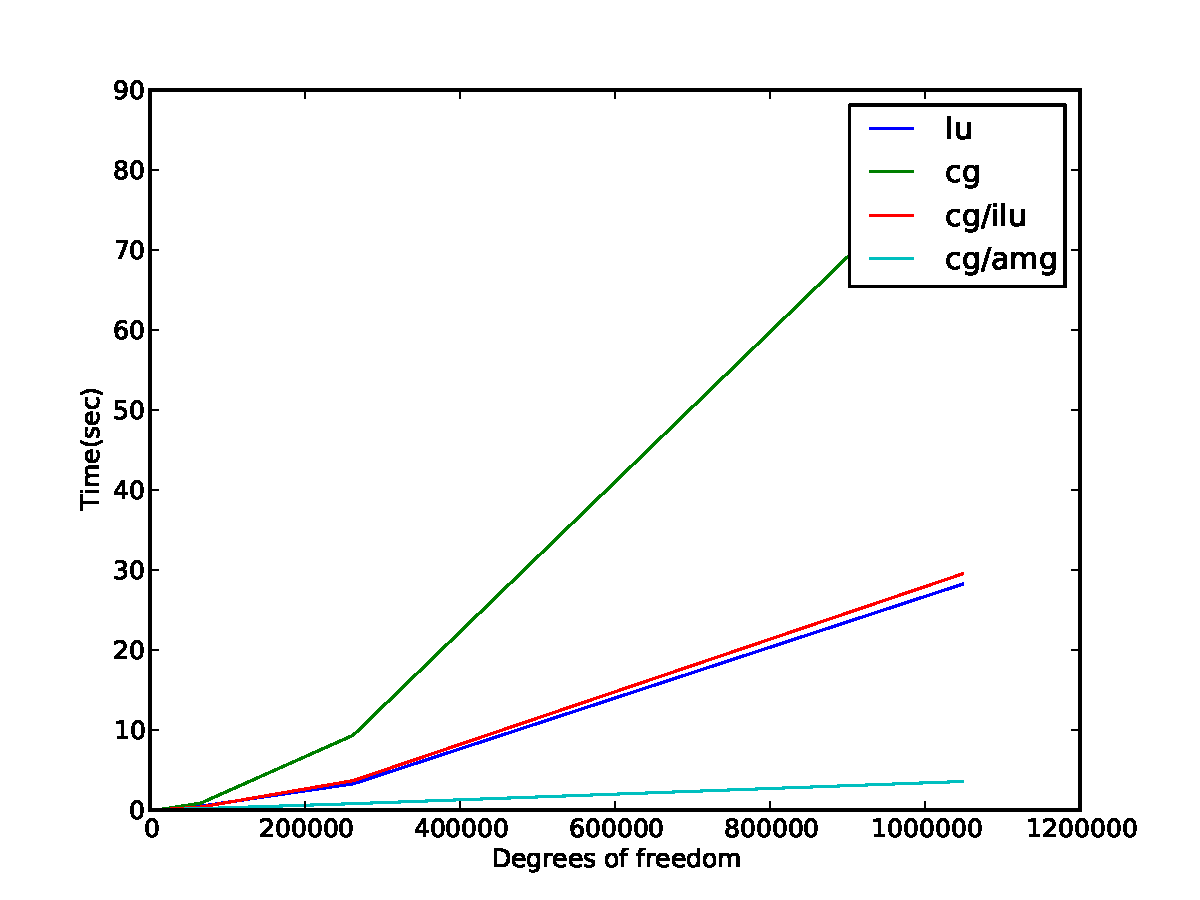
\includegraphics[width=8cm, height=7cm]{chapters/iterative_methods/plots/cpu_time_comparison_plot.pdf}
\caption{CPU time (in seconds) for solving a linear system of equation with $N$ degrees of freedom (x-axis) 
             for different solvers} 
\label{fig:CPU_time}
\end{figure}

\begin{python}
from dolfin import *
import time
lu_time = []; cgamg_time = []
cg_time = []; cgilu_time = []
Ns = []

parameters["krylov_solver"]["relative_tolerance"] = 1.0e-8
parameters["krylov_solver"]["absolute_tolerance"] = 1.0e-8
parameters["krylov_solver"]["monitor_convergence"] = False
parameters["krylov_solver"]["report"] = False
parameters["krylov_solver"]["maximum_iterations"] = 50000

def solving_time(A,b, solver):
  U = Function(V)
  t0 = time.time()
  if len(solver) == 2: 
    solve(A, U.vector(), b, solver[0], solver[1]);
  else: 
    solve(A, U.vector(), b, solver[0]);
  t1 = time.time()
  return t1-t0

for N in [32, 64, 128, 256, 512, 1024]:

  Ns.append(N)

  mesh = UnitSquare(N, N)
  print " N ", N, " dofs ", mesh.num_vertices()
  V = FunctionSpace(mesh, "Lagrange", 1)
  u = TrialFunction(V)
  v = TestFunction(V)

  f = Expression("sin(x[0]*12) - x[1]")
  a = u*v*dx  + inner(grad(u), grad(v))*dx
  L = f*v*dx

  A = assemble(a)
  b = assemble(L)
  
  t2 = solving_time(A,b, ["lu"])
  print "Time for lu ", t2
  lu_time.append(t2)
  
  t2 = solving_time(A, b, ["cg"])
  print "Time for cg ", t2
  cg_time.append(t2)

  t2 = solving_time(A, b, ["cg", "ilu"])
  print "Time for cg/ilu ", t2
  cgilu_time.append(t2)

  t2 = solving_time(A, b, ["cg", "amg"])
  print "Time for cg/amg ", t2
  cgamg_time.append(t2)


import pylab

pylab.plot(Ns, lu_time)
pylab.plot(Ns, cg_time)
pylab.plot(Ns, cgilu_time)
pylab.plot(Ns, cgamg_time)  
pylab.xlabel('Unknowns')
pylab.ylabel('Time(sec)')
pylab.legend(["lu", "cg", "cg/ilu", "cg/amg"])
pylab.show()

pylab.loglog(Ns, lu_time)
pylab.loglog(Ns, cg_time)
pylab.loglog(Ns, cgilu_time)
pylab.loglog(Ns, cgamg_time)
pylab.legend(["lu", "cg", "cg/ilu", "cg/amg"])
pylab.savefig('tmp_cpu.pdf')
pylab.show()
\end{python}
\end{example}

When we employ iterative methods, we need to specify the convergence criterion. This is often 
not an easy task. We have the continuous solution $u$, the discrete solution $u_h$, and the
appropriate discrete solution, $u_h^n$ found by an iterative method at iteration $n$.  
Obviously, we may estimate the error as
\[
\|u-u^n_h\| \le \|u-u_h\| + \|u_h-u_h^n\|, 
\]
and it does make sense that the values of 
$\|u-u_h\|$ and $\|u_h-u_h^n\|$ are balanced. Still both terms may be hard to estimate in 
challenging applications. In practice, an appropriate convergence criterion is usually 
found by trial and error by choosing a stopping criterion based on the residual.   
Let us therefore consider a concrete example and consider $\|u-u^n_h\|$ 
as a function of the mesh resolution and a varying convergence criterion. 


\begin{table}
\begin{tabular}{c|ccccc}
\hline 
$\epsilon\backslash$ N & 64 & 128 & 256 & 512 & 1024 \\ \hline 
1.0e-1 &  1.3e-02 (1.1e-02) &  1.4e-02 (3.5e-02) &  8.8e-03 (1.4e-01) &  3.4e-03 (5.9e-01) &  1.1e-02 (2.5e+00) \\ 
1.0e-2 &  1.2e-03 (1.0e-02) &  2.0e-03 (3.7e-02) &  1.3e-03 (1.5e-01) &  3.5e-03 (5.8e-01) &  3.7e-04 (2.7e+00) \\ 
1.0e-3 &  3.6e-04 (1.1e-02) &  3.1e-04 (3.9e-02) &  2.6e-04 (1.6e-01) &  2.7e-04 (6.3e-01) &  3.7e-04 (2.7e+00) \\ 
1.0e-4 &  3.4e-04 (1.2e-02) &  8.5e-05 (4.5e-02) &  2.4e-05 (1.8e-01) &  3.4e-05 (6.7e-01) &  1.4e-05 (2.9e+00) \\ 
1.0e-5 &  3.4e-04 (1.2e-02) &  8.4e-05 (4.7e-02) &  2.1e-05 (1.9e-01) &  5.4e-06 (7.6e-01) &  2.8e-06 (3.1e+00) \\ 
1.0e-6 &  3.4e-04 (1.3e-02) &  8.4e-05 (5.0e-02) &  2.1e-05 (2.1e-01) &  5.3e-06 (8.1e-01) &  1.3e-06 (3.3e+00) \\ 
\end{tabular}
\caption{The error $\|u-u^n_h\|$ and corresponding CPU time in parentesis when solving a Poisson problem
with homogenuous Dirichlet conditions. } 
\label{conv:res:error}. 
\end{table}



Table \ref{conv:res:error} shows the error and the corresponding CPU timings when solving a Poisson problem
at various resolutions and convergence criteria. 
Here, the convergence criteria is chosen as reducing the relative residual, i.e., $\frac{\|r_k\|}{\|r_0\|}$
by the factor $\epsilon$. This convergence criteria is very common, in particular for stationary problems.  
There are several things to note here. For coarse resolution, \emp{N=64}, the error stagnates somewhere
between $1.0e-3$ and $1.0e-4$ and this stagnation marks where an appropriate stopping criteria is.   
It is however worth noticing that solving it to a criteria that is 
$1.0e-6$ is actually only about 30\% more computationally demanding than $1.0e-3$. This is due to the
fact that we have a very efficient method that reduces the error by about a factor 10 per iteration.   
If we consider the fine resolution, \emp{N=1024}, we see that the stagnation happens later and that
we may not even have reached the stagnating point even at $\epsilon=1.0e-6$. We also notice that 
the decreasing $\epsilon$ in this case only lead to a moderate growth in CPU time.   
If we look closer at the table, we find that the stagnation point follows a staircase pattern. 
The code used to generate the table is as follows: 

\begin{python}
from dolfin import *

def boundary(x, on_boundary):
    return on_boundary

parameters["krylov_solver"]["relative_tolerance"] = 1.0e-18 
parameters["krylov_solver"]["absolute_tolerance"] = 1.0e-18 
parameters["krylov_solver"]["monitor_convergence"] = True 
parameters["krylov_solver"]["report"] = True 
#parameters["krylov_solver"]["maximum_iterations"] = 50000 
epss = [1.0e-1, 1.0e-2, 1.0e-3, 1.0e-4, 1.0e-5, 1.0e-6]
data = {}
Ns= [64, 128, 256, 512, 1024]
#Ns= [8, 16, 32, 64]
for N in Ns:
  for eps in epss:  
    parameters["krylov_solver"]["relative_tolerance"] = eps 

    mesh = UnitSquareMesh(N, N)
    V = FunctionSpace(mesh, "P", 1)
    u = TrialFunction(V)
    v = TestFunction(V)

    u_ex = Expression("sin(3.14*x[0])*sin(3.14*x[1])", degree=3) 
    f = Expression("2*3.14*3.14*sin(3.14*x[0])*sin(3.14*x[1])", degree=3) 
    a = inner(grad(u), grad(v))*dx  
    L = f*v*dx 

    U = Function(V)

    A = assemble(a) 
    b = assemble(L)

    bc = DirichletBC(V, u_ex, boundary)
    bc.apply(A)
    bc.apply(b) 

    t0 = time()
    solve(A, U.vector(), b, "gmres", "amg")
    t1 = time()

    cpu_time = t1-t0
    error_L2 = errornorm(u_ex, U, 'L2', degree_rise=3)
    data[(N, eps)] = (error_L2, cpu_time) 

for eps in epss:  
  for N in Ns:
    D1, D2 = data[(N, eps)]
    print " %3.1e (%3.1e) " % (D1, D2), 
    print ""
	
\end{python}

\begin{example}{\textbf{Eigenvalues of the preconditioned system.}}
It is often interesting to assess the condition number of the 
preconditioned system, $BA$. If the preconditioner is a matrix and the
size of the system is moderate we may be able to estimate the condition
number of $BA$ using NumPy, Matlab or Octave. However, when our preconditioner
is an algorithm representing a linear operator, such as in the case
of multigrid, then this is not possible. However, as described in~\cite{saad2003iterative}, 
egenvalues may be estimated as a bi-product of the Conjugate Gradient method. Without
going into the algorithmic details of the implmementation, we mention that
this is implemented in the FEniCS module \emp{cbc.block}, see~\cite{mardal2012block}.      
The following code shows the usage.  
\begin{python}
from dolfin import *
from block.iterative import ConjGrad
from block.algebraic.petsc import ML
from numpy import random

def boundary(x, on_boundary):
    return on_boundary

class Source(Expression):
    def eval(self, values, x):
        dx = x[0] - 0.5; dy = x[1] - 0.5
        values[0] = 500.0*exp(-(dx*dx + dy*dy)/0.02)

Ns = [8, 16, 32, 64, 128, 256, 512, 1024]
for N in Ns: 
    mesh = UnitSquareMesh(N,N)
    V = FunctionSpace(mesh, "CG", 1)

    # Define variational problem
    v = TestFunction(V)
    u = TrialFunction(V)
    f = Source(degree=3)
    a = dot(grad(v), grad(u))*dx
    L = v*f*dx 
    bc = DirichletBC(V, Constant(0), boundary)

    # Assemble matrix and vector, create precondition and start vector 
    A, b = assemble_system(a,L, bc)
    B = ML(A)
    x = b.copy()
    x[:] = random.random(x.size(0))

    # solve problem and print out eigenvalue estimates. 
    Ainv = ConjGrad(A, precond=B, initial_guess=x, tolerance=1e-8, show=2)
    x = Ainv*b
    e = Ainv.eigenvalue_estimates()
    print "N=%d iter=%d K=%.3g" % (N, Ainv.iterations, e[-1]/e[0])
\end{python}
In this example we see that the condition number increases logaritmic from 1.1 to 2.1 as the \emp{N}
increases from 8 to 1024. The \emp{AMG} preconditioner has better performance and does
not show logaritmic growth. For indefinite symmetric systems, the \emp{CGN} method provides
the means for estimating the condition number, c.f., the \emp{cbc.block} documentation.    
\end{example}

\subsection{Insight from Functional Analysis}
In the previous Chapters \ref{chap-conv} and \ref{chap-stokes}
we have discussed the well-posedness of the convection-diffusion
equations and the Stokes problem. In both cases, the problems 
were well-posed - meaning that the differential operators
as well as their inverse were continuous. 
However, when we discretize the problems we get matrices
where the condition number grows to infinity as the element size goes to  
zero. This seem to contradict the well-posedness of our discrete problems
and may potentially destroy both the accuracy and efficiency 
of our numerical algorithms. Functional analysis explains this 
apparent contradiction and explains how the problem is circumvented by 
preconditioning.   

Let us now consider the seeming contradiction in more precise
mathematical detail for the Poisson problem 
with homogeneous Dirichlet conditions:  
Find $u$ such that 
\begin{eqnarray}
- \Delta u &=& f, \quad \text{ in } \Omega,  \\     
u &=& 0, \quad \text{ on } \partial \Omega .  
\end{eqnarray}

We know from Lax-Milgram's theorem that 
the weak formulation of this problem: 
Find $u\in H^1_0$ such that 
\[
a(u, v) = b(v), \quad \forall v\in H^1_0 .   
\]
where 
\begin{eqnarray}
a(u,v) &=& \int_\Omega \nabla u \cdot \nabla v \, dx, \\   
b(v)   &=& \int_\Omega  f  v \, dx,   
\end{eqnarray}
is well-posed because 
\begin{eqnarray}
a(u,u) &\ge& \alpha |u|^2_{1} \ , \quad \forall u \in H^1_0  \\ 
a(u,v) &\le& C |u|_{1} |v|_{H_0^1} \quad \forall u,v \in H^1_0   \ . 
\end{eqnarray}
Here $|\cdot|_{1}$ denotes the $H^1$ semi-norm which is known to 
be a norm on $H^1_0$ due to Poincare.  
The well-posedness is in this case stated as
\begin{equation}
|u|_{H_0^1} \le \frac{1}{\alpha} \|f\|_{H^{-1}} .  
\end{equation}
In other words, $-\Delta$ takes a function $u$ in $H^1_0$ and  
returns a function $f=-\Delta u$ which is in $H^{-1}$. We
have that $\|f\|_{-1} = \|-\Delta u\|_{-1} \le C \|u\|_1$.     
Also, $-\Delta^{-1}$ takes a function $f$ in $H^{-1}$ and  
returns a function $u=(-\Delta)^{-1} f$ which is in $H^1_0$. We
have that $\|u\|_{1} = \|(-\Delta)^{-1} f\|_{1} \le \frac{1}{\alpha} \|f\|_{-1}$.     
In fact, in this case $\alpha=C=1$. 

This play with words and symbols may be formalized by using operator norms that
are equivalent with matrix norms. Let $B \in \R^{n,m}$ then
\[    
\|B\|_{\mathcal{L}(\R^m, \R^n)} = \max_{x\in\R^m} \frac{\Vert B x\Vert_{\R^n}}{\Vert x \Vert_{\R^m}}   
\]
Here $\mathcal{L}(\R^m, \R^n)$ denotes the space of all $m\times n$ matrices. 

Analogously, we may summarize the mapping properties of $-\Delta$ and  $(-\Delta)^{-1}$ 
in terms of the conditions of Lax-Milgram's theorem as  
\begin{equation} 
\label{boundeddelta}
\|-\Delta\|_{\mathcal{L}(H^1_0, H^{-1})} \le C
\quad \text{ and } \quad  
\|(-\Delta)^{-1}\|_{\mathcal{L}(H^{-1}, H^1_0) } \le \frac{1}{\alpha} \ . 
\end{equation}
where ${\mathcal{L}(X, Y)}$ denotes the space of bounded linear operators mapping
$X$ to $Y$.  
In other words, $-\Delta$ is a bounded linear map from
$H^1_0$ to $H^{-1}$ and 
$(-\Delta)^{-1}$ is a bounded linear map from
$H^{-1}$ to $H^1_0$. 
This is a crucial observation
in functional analysis that, in contrast to the case of  
a matrix which is  a bounded linear map from $\R^n$ to $\R^m$, 
an operator may be map from one space to another. 

From Chapter \ref{chap-sobolev} we know that the eigenvalues
and eigenvectors of $-\Delta$ with homogeneous Dirichlet
conditions on the unit interval in 1D are
$\lambda_k=(\pi k)^2$ and $e_k = sin(\pi k x)$, respectively. 
Hence the eigenvalues of $-\Delta$ obviously tend to $\infty$
as $k$ grows to $\infty$ and similarly the eigenvalues
of $(-\Delta)^{-1}$ accumulate at zero as $k\rightarrow \infty$.  
Hence the spectrum of $-\Delta$ is unbounded and the 
spectrum of $(-\Delta)^{-1}$ has an accumulation point at zero.  
Still, the operator $-\Delta$ and its inverse are bounded
from a functional analysis point of view, in the sense of 
\eqref{boundeddelta}.  


Let us for the moment assume that we have access to an operator $B$ with mapping
properties that are inverse to that of $A=-\Delta$, i.e., 
\begin{equation} 
\label{boundedB}
\|B\|_{\mathcal{L}(H^{-1}, H^1_0) } \  
\quad \text{ and } \quad  
\|B^{-1}\|_{\mathcal{L}(H^1_0, H^{-1})} . 
\end{equation}
Then it follows directly that 
\begin{equation} 
\label{boundeddelta}
\|B A\|_{\mathcal{L}(H^1_0, H^1_0) } \  
\quad \text{ and } \quad  
\|(B A)^{-1}\|_{\mathcal{L}(H^1_0, H^1_0)} . 
\end{equation}
and the condition number 
\[
\kappa(BA) = \frac{\max_i \lambda_i (BA)}{\min _i \lambda_i (BA)} =    \|B A\|_{\mathcal{L}(H^1_0, H^1_0) }   \|(B A)^{-1}\|_{\mathcal{L}(H^1_0, H^1_0)}
\]
would be bounded.  
In the discrete case, the mapping property \eqref{boundedB} translates to the fact that  $B$ should be spectrally equivalent with the inverse of $A$ 
when $B$ and $A$ are both positive.  

While the above discussion is mostly just a re-iteration of the concept of spectral equivalence in the discrete case 
when the PDEs are elliptic, 
the insight from functional analysis can be powerful for systems of PDEs. 
Let us consider the Stokes problem from Chapter \ref{chap-stokes}.  
The problem reads: 
\[
\mathcal{A}  
\left[ 
\begin{array}{c}
u \\ p  
\end{array}
\right]
=
\left[ 
\begin{array}{cc}
-\Delta & -\nabla \\  
\nabla\cdot & 0  
\end{array}
\right]
\left[ 
\begin{array}{c}
u \\ p  
\end{array}
\right]
=
\left[ 
\begin{array}{c}
u \\ p  
\end{array}
\right]
\]
As discussed in Chapter \ref{chap-stokes} 
\[
\mathcal{A} : H^1_0 \times L^2 \rightarrow   H^{-1} \times L^2 
\]
was a bounded linear mapping with a bounded inverse.  
Therefore, a preconditioner can be constructed as 
\[
\mathcal{B}
= 
\left[ 
\begin{array}{cc}
(-\Delta)^{-1} & 0 \\  
0 & I  
\end{array}
\right]
\]
Clearly 
\[
\mathcal{B}:  H^{-1} \times L^2 \rightarrow H^1_0 \times L^2   
\]
and is therefore a suitable preconditioner. However, we also notice that
$\mathcal{A}$ and $\mathcal{B}^{-1}$ are quite different. 
$\mathcal{A}$ is indefinite and has positive and negative egenvalues, while
$\mathcal{B}$ is clearly positive. Hence, the operators are not spectrally equivalent.    
Exercise \ref{ex:stokes} looks deeper into this construction of preconditioners
for Stokes problem. A more comprehensive description of this technique
can be found in \cite{mardal2011preconditioning}.



\section{Exercises}

\begin{exercise}
\label{ex:nnz}
Estimate ratio of non-zeros per unknown of the stiffness matrix on the unit square   
with Lagrangian elements of order 1, 2, 3 and 4. Hint: the 
number of non-zeros can be obtained from the function 'nnz' of a matrix object.  
\end{exercise}

\begin{exercise}
\label{ex:eig:1D2D3D}
Compute the smallest and largest eigenvalues of the mass matrix and 
the stiffness matrix in 1D, 2D and 3D. Assume that
the condition number is on the form  
$\kappa \approx C h^\alpha$, where $C$ and $\alpha$ may
depend on the number of dimentions in space.   
Finally, compute the corresponding condition numbers.  
Does the condition number have the same dependence on 
the number of dimentions in space?  
\end{exercise}

\begin{exercise}
\label{ex:eig:1D2D3D:order}
Repeat Exercise \ref{ex:eig:1D2D3D} but with Lagrange elements of order 1, 2 and 3.  
How does the order of the polynomial affect the eigenvalues and condition numbers. 
\end{exercise}


\begin{exercise}
Compute the eigenvalues the discretized Stokes problem
using Taylor-Hood elements. Note that the problem
is indefinite and that there are both positive and 
negative eigenvalues. An appropriate condition number
is:   
\[
\kappa = \frac{ \max_i |\lambda_i |}{ \min_i | \lambda_i|}
\]
where $\lambda_i$ are the eigenvalues of $A$. 
Compute corresponding condition numbers for the Mini and Crouzeix-Raviart 
elements. Are the condition numbers similar?  
\end{exercise}

\begin{exercise}
Implement the Jacobi iteration for a 1D Poisson problem with homogeneous
Dirichlet conditions. Start the iteration with an initial random vector and
estimate the number of iterations required to reduce the $L_2$ norm of the  residual
with a factor $10^4$. For relevant code see Example \ref{example:CPU_time}.
\end{exercise}


\begin{exercise}
\label{ex:poisson}
Test CG method without preconditioer, with ILU preconditioner and with AMG preconditioner 
for the Poisson problem in 1D and 2D with homogeneous Dirichlet conditions,  with respect
to different mesh resolutions. Do some of the iterations suggest spectral equivalence?
\end{exercise}

\begin{exercise}
\label{ex:conv}
Test CG, BiCGStab, GMRES with ILU, AMG, and Jacobi preconditioning for 
\begin{eqnarray*}
-\mu\Delta u + v\nabla u   &=& f \quad \textrm{in}\ \Omega\\
u&=& 0 \quad \textrm{on}\ \partial\Omega
\end{eqnarray*}
Where $\Omega$ is the unit square, $v=c\, sin(7 x)$, and $c$ varies as $1, 10, 100, 1000, 10 000$ and
the mesh resolution $h$ varies as $1/8, 1/16, 1/32, 1/64$. You may assume homogeneous Dirichlet conditions.  

\end{exercise}



\begin{exercise}
\label{ex:stokes}
The following code snippet shows the assembly of the matrix and preconditioner
for a Stokes problem: 
\begin{python} 
a = inner(grad(u), grad(v))*dx + div(v)*p*dx + q*div(u)*dx
L = inner(f, v)*dx

# Form for use in constructing preconditioner matrix
b = inner(grad(u), grad(v))*dx + p*q*dx

# Assemble system
A, bb = assemble_system(a, L, bcs)

# Assemble preconditioner system
P, btmp = assemble_system(b, L, bcs)

# Create Krylov solver and AMG preconditioner
solver = KrylovSolver("tfqmr", "amg")

# Associate operator (A) and preconditioner matrix (P)
solver.set_operators(A, P)

# Solve
U = Function(W)
solver.solve(U.vector(), bb)
\end{python} 
Here, "tfqmr" is a variant of the Minimal residual method and "amg" is an algebraic 
multigrid implementation in HYPRE. Test, by varying the mesh resolution, whether
the code produces an order--optimal preconditioner.  
HINT: You might want to change the "parameters" as done
in Example \ref{example:CPU_time}: 
\begin{python}
# Create Krylov solver and AMG preconditioner
solver = KrylovSolver("tfqmr", "amg")
solver.parameters["relative_tolerance"] = 1.0e-8
solver.parameters["absolute_tolerance"] = 1.0e-8
solver.parameters["monitor_convergence"] = True
solver.parameters["report"] = True
solver.parameters["maximum_iterations"] = 50000
\end{python}
\end{exercise}

\begin{exercise}
\label{ex:stokes}
Consider the mixed formulation of linear elasticity that
is appropriate when $\lambda$ is large compared to $\mu$. That is, 
\begin{python} 
a = inner(grad(u), grad(v))*dx + div(v)*p*dx + q*div(u)*dx - 1/lam*p*q*dx 
L = inner(f, v)*dx
\end{python}
Create two preconditioners: 
\begin{python} 
b1 = inner(grad(u), grad(v))*dx + p*q*dx
b2 = inner(grad(u), grad(v))*dx + 1/lam*p*q*dx
\end{python} 
Compare the efficiency of the different preconditioners when increasing
the resolution and when $\lambda\rightarrow\infty$. 
Can you explain why the first preconditioner is the best?
\end{exercise}



%Suggestions to exercise:
%Show that the eigenvalues to the Jacobi(and relaxed) are ...
%Show/prove the "show this" 

%------------------------------------------------------------------------------

%Triks fra Adrian
%\begin{align}
%Lu =&\left\{ \begin{array}{lr}  -u(x)'' &= f(x) \quad \foralls x \in \Omega\\ u(0) = u(1) &= 0  \end{array}% \right. \end{align}

        \fenicschapter{Linear elasticity and singular problems}
              {Linear elasticity and singular problems}
              {Linear elasticity and singular problems} 
              {Anders Logg, Kent--Andre Mardal} 
              {chap-elasticity}   
\label{chap-elasticity}

\section{Introduction} 

Let us consider an elastic body $\Omega_0$ that is being deformed under a load
to become $\Omega$.
the deformation $\chi$ of a body in the undeformed state $\Omega_0$ to deformed state $\Omega$. A point in the body has then moved
\begin{align}
u = x - X,
\end{align}
by definition this is \emph{displacement field}. An illustration is shown in Figure \ref{el:def}. 

\begin{figure}[h!]

\begin{center}
  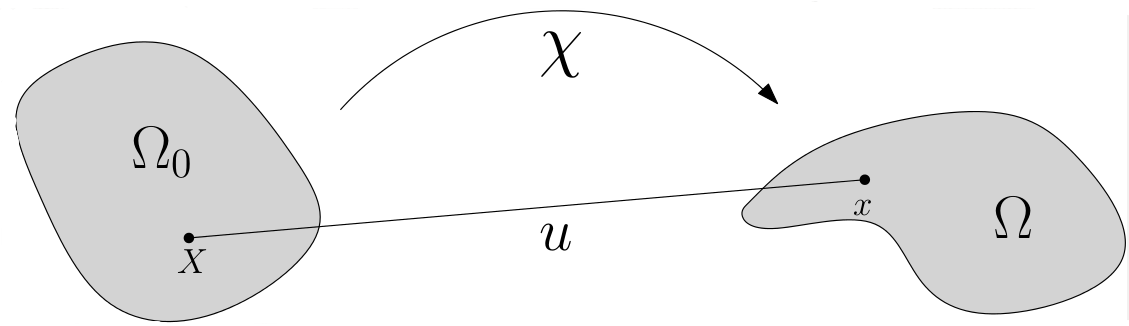
\includegraphics[scale=0.25]{chapters/elasticity/displace.png}
  \end{center}
\caption{Deforming body and displacement vector $u$.}
\label{el:def}
\end{figure}

Here, the domain $\Omega_0 \subset \R^3$. From continuum mechanics, the elastic deformation is modelled by the stress tensor $\sigma$ which is a symmetric $3\times 3$ tensor. 
In equilibrium (i.e. no accelration terms) the Newton's second law states 
the balance of forces as: 
\begin{eqnarray*}  
\operatorname{div} \sigma &=& f, \quad\mbox{in}\ \Omega ,  \\ 
\sigma \cdot n &=& g, \quad\mbox{on}\ \partial \Omega,   
\end{eqnarray*}  
where $f$ and $g$ are body and surface forces,  respectively and $n$ is the outward normal vector.   

For small deformations of an isotropic media, Hooke's law is a good approximation. 
Hooke's law states that 
\[
\sigma = 2 \mu \epsilon(u) + \lambda \operatorname{tr}(\epsilon(u)) \delta.  
\]
Here, $\epsilon(u)$ is the strain tensor or the symmetric gradient: 
\[
\epsilon(u) = \frac{1}{2} (\nabla u + (\nabla u)^T),   
\]
$\mu$ and $\lambda$ are the Lame constants, $\operatorname{tr}$ is the trace operator (the sum of the diagonal matrix
entries), $u$ is the displacement, and  
\[
\delta = \left[ \begin{array}{ccc} 1 & 0 & 0 \\ 0 & 1 & 0 \\ 0 & 0 & 1 \end{array} \right].
\]

From Newton's second law and Hooke's law we arrive directly at the equation of linear elasticity: 
\begin{align}
\label{el:eq}
-2 \mu (\nabla \cdot \epsilon (u)) - \lambda \nabla (\nabla \cdot u) = f.
\end{align}
The equation of linear elasticity \eqref{el:eq} is an elliptic equation, but there are crucial differences between this equation
and a standard elliptic equation like $-\Delta u = f$. These differences often cause
problems in a numerical setting. To explain the numerical issues we will here
focus on the differences between the three operator:
\begin{enumerate}
\item $-\Delta  = \nabla\cdot\nabla  = \operatorname{div}\operatorname{grad} $,
\item $\nabla \cdot \epsilon = \nabla\cdot(\frac{1}{2}(\nabla + (\nabla^T))$,
\item $\nabla \cdot \operatorname{tr} \epsilon = \nabla \nabla \cdot = \operatorname{grad} \operatorname{div}$. 
\end{enumerate}
In particular, the differences between the operators in 1. and 2. is that $\nabla \cdot \epsilon$ has a
larger kernel than $-\Delta$. The kernel consists of rigid motions and this leads to the usage of
of one of Korn's lemmas.
This is the subject of Section \ref{el:korn}. The kernel of the operators  
$\operatorname{grad} \operatorname{div}$ and $\operatorname{div}\operatorname{grad}$
are also different but here in fact the kernel of $\operatorname{grad} \operatorname{div}$ is infinite dimentional
and this has different consequences for the numerical algorithms which not necessarily pick up this kernel at
all. This is discussed in Section \ref{el:lock}.

\section{The operator $\nabla \cdot \epsilon$ and rigid motions}
\label{el:korn}
The challenge with the handling of the $\nabla \cdot \epsilon$ operator is the
handling of the singularity in the case of pure Neumann conditions. Let us therefore
start with the simpler problem of the Poisson problem with Neumann conditions, i.e., 
\begin{eqnarray}
-\Delta u &=& f, \quad \mbox{in}\ \Omega, \\
\frac{\partial u}{\partial n} &=& g, \quad \mbox{on}\ \partial \Omega .
\end{eqnarray}
It is easy to see that this problem is singular: Let $u$ be a solution
of the above equation, then $u+C$ with $C\in\R$ is also a solution because
$-\Delta u = \Delta (u + C) = f$ and
$\frac{\partial u}{\partial n} = \frac{\partial (u+C)}{\partial n} = g$.
Hence, the solution is only determined up to a constant. This means
that  the kernel  is 1-dimentional.

A proper formulation of the above problem can be obtained by using the method
of Lagrange multipliers to fixate the element of the 1-dimentional
kernel. The following weak formulation is well-posed:
Find $u\in H^1$ and $\lambda \in \R$ such that
\begin{eqnarray}
\label{poisson:neu1}
a(u,v) + b(\lambda, v) &=& f(v) \quad \forall v\in H^1 \\
\label{poisson:neu2}
b(u, \gamma) &=& 0, \quad \forall \gamma \in \R.
\end{eqnarray}
Here,
\begin{eqnarray}
\label{poisson:neu3}
a(u,v) &=& (\nabla u, \nabla v), \\
\label{poisson:neu4}
b(\lambda, v) &=& (\lambda, v), \\
\label{poisson:neu5}
f(v) &=& (f,v) + \int_{\partial \Omega} g v ds .
\end{eqnarray}
Hence, the method of Lagrange multipliers turns the original problem
into a saddle problem similar that in Chapter \ref{chap-stokes}. However,
in this case the Brezzi conditions are easily verified. We remark
however that this formulation makes the problem indefinite rather
than positive definite and for this reason alternative techniques
such as pin-pointing is often used instead. We will not avocate this
approach as it often causes numerical problems. Instead, we
include a code example that demonstrate how this problem can
be implemented with the method of Lagrange multipliers in FEniCS.
\begin{python}
from dolfin import *

mesh = UnitSquareMesh(64, 64)

# Build function space with Lagrange multiplier
P1 = FiniteElement("Lagrange", mesh.ufl_cell(), 1)
R = FiniteElement("Real", mesh.ufl_cell(), 0)
W = FunctionSpace(mesh, P1 * R)

# Define variational problem
(u, c) = TrialFunction(W)
(v, d) = TestFunctions(W)
f = Expression("10*exp(-(pow(x[0] - 0.5, 2) + pow(x[1] - 0.5, 2)) / 0.02)", degree=2)
g = Expression("-sin(5*x[0])", degree=2)
a = (inner(grad(u), grad(v)) + c*v + u*d)*dx
L = f*v*dx + g*v*ds

# Compute solution
w = Function(W)
solve(a == L, w)
(u, c) = w.split()

# Plot solution
plot(u, interactive=True)
\end{python}

The kernel of the $\epsilon$ operator is the space of rigid motions, $\operatorname{RM}$. The space consists of translations and rotations. Rigid motions
are on the following form in 2D and 3D:
\begin{eqnarray}
\operatorname{RM}_{2D} &=& \left[\begin{array}{c} a_0 \\ a_1 \end{array}\right] + a_2 \left[\begin{array}{c} -y\\ x\end{array} \right], \\
\operatorname{RM}_{3D} &=& \left[\begin{array}{c} a_0 \\ a_1 \\ a_2 \end{array}\right]
     + \left[\begin{array}{ccc} 0 & a_3 & a_4 \\
                               -a_3 & 0 & a_5\\
                               -a_4 & -a_5 & 0
             \end{array}\right]
 \left[\begin{array}{c}
x\\ y \\ z \end{array} \right].
\end{eqnarray}
Hence, the kernel in 2D is three-dimentional and may be expressed as above in terms of the degrees of freedom $(a_0, a_1, a_2)$ whereas the kernel in 3D is six-dimentional $(a_0, \ldots, a_5)$.

The Korn's lemmas states suitable conditions for solvability. Here, we include two of the three inequalities typically
listed.  
\begin{itemize}
\item The first lemma: For all $u\in H^1 \backslash \operatorname{RM}$ we have that $\|\epsilon(u)\| \ge C \|u\|_1$.
\item The second lemma: For all $u\in H^1_0 $ we have that $\|\epsilon(u)\| \ge C \|u\|_1$. 
\end{itemize}
These lemmas should be compared with the Poincare's lemma and the equivalence of the $|\cdot|_1$ and $\|\cdot\|_1$ norms.
The second lemma states that when we have homogenous Dirichlet conditions we obtain a well-posed problem
in a similar manner as for a standard elliptic problem. This case is often called fully-clamped conditions.
For the Neumann problem, however, coersivity is not obtained unless we remove the complete set of rigid motions
for the function space used for trial and test functions. Removing the rigid motions is most easily done
by using the method of Lagrange multipliers. 

Let us now consider a weak formulation of the linear elasticity problem and describe how to implement
it in FEniCS. For now we consider the case where $\lambda$ and $\mu$ are of comparable magnitude. In
the next section we consider the case where $\lambda \gg \mu$.
The weak formulation of the linear elasticity problem is:
Find $u\in H^1$ and $r \in \operatorname{RM}$ such that
\begin{eqnarray}
\label{el:lm:1}
a(u,v) + b(r, v) &=& f(v), \quad \forall v\in H^1, \\
\label{el:lm:2}
b(s,u) &=& 0, \quad \forall s \in \operatorname{RM}.
\end{eqnarray}
Here,
\begin{eqnarray}
a(u,v) &=& \mu (\epsilon(u), \epsilon(v)) + \lambda (\operatorname{div} u, \operatorname{div} v)  \\
b(r, v) &=& (r, v), \\
f(v) &=& (f,v) + \int_{\partial \Omega} g v ds .
\end{eqnarray}

As we know from Chapter \ref{chap-stokes}, this is a saddle point problem and we need to
comply with the Brezzi conditions. Verifying these conditions are left as Exercise \ref{ex:kornbrezzi}.

\begin{example}
Our brain and spinal cord is floating in a water like fluid called the cerebrospinal fluid.
While the purpose of this fluid is not fully known, it is known that the pressure in
the fluid oscillates with about 5-10 mmHg during a cardic cycle which is approximately one
second, c.f., e.g., ~\cite{eide2016correlation}. The Youngs' modulus has been estimated 16 kPa
and 1 mmHg $\approx$ 133 Pa, c.f., e.g., ~\cite{stoverud2016poro}. To compute the deformation of the brain during a
cardiac cycle we consider solve the linear elasticity problem with Neumann condtions
set as pressure of 1 mm Hg and ... The following code shows the implmentation in FEniCS.
The mesh of the brain was in this case obtained from a T1 magnetic ressonance image
and segmentation was performed by using FreeSurfer. 

\begin{python}
from fenics import *

mesh = Mesh('mesh/res32.xdmf')	# mm

plot(mesh,interactive=True)

# Since the mesh is in mm pressure units in pascal must be scaled by alpha = (1e6)**(-1)
alpha = (1e6)**(-1)

# Mark boundaries
class Neumann_boundary(SubDomain):
	def inside(self, x, on_boundry):
		return on_boundry

mf = FacetFunction("size_t", mesh)
mf.set_all(0)

Neumann_boundary().mark(mf, 1)
ds = ds[mf]

# Continuum mechanics
E = 16*1e3 *alpha
nu = 0.25
mu, lambda_ = Constant(E/(2*(1 + nu))), Constant(E*nu/((1 + nu)*(1 - 2*nu)))
epsilon = lambda u: sym(grad(u))

p_outside = 133 *alpha
n = FacetNormal(mesh)
f = Constant((0, 0, 0))

V = VectorFunctionSpace(mesh, "Lagrange", 1)

# --------------- Handle Neumann-problem --------------- #
R = FunctionSpace(mesh, 'R', 0)        		 # space for one Lagrange multiplier
M = MixedFunctionSpace([R]*6)          		 # space for all multipliers
W = MixedFunctionSpace([V, M])
u, rs = TrialFunctions(W)
v, ss = TestFunctions(W)

# Establish a basis for the nullspace of RM
e0 = Constant((1, 0, 0))				# translations
e1 = Constant((0, 1, 0))
e2 = Constant((0, 0, 1))

e3 = Expression(('-x[1]', 'x[0]', '0')) # rotations
e4 = Expression(('-x[2]', '0', 'x[0]'))
e5 = Expression(('0', '-x[2]', 'x[1]'))
basis_vectors = [e0, e1, e2, e3, e4, e5]

a = 2*mu*inner(epsilon(u),epsilon(v))*dx + lambda_*inner(div(u),div(v))*dx
L = inner(f, v)*dx + p_outside*inner(n,v)*ds(1)

# Lagrange multipliers contrib to a
for i, e in enumerate(basis_vectors):
	r = rs[i]
	s = ss[i]
	a += r*inner(v, e)*dx + s*inner(u, e)*dx

# -------------------------------------------------------- #

# Assemble the system
A = PETScMatrix()
b = PETScVector()
assemble_system(a, L, A_tensor=A, b_tensor=b)

# Solve
uh = Function(W)
solver = PETScLUSolver('mumps') # NOTE: we use direct solver for simplicity
solver.set_operator(A)
solver.solve(uh.vector(), b)

# Split displacement and multipliers. Plot
u, ls = uh.split(deepcopy=True) 
plot(u, mode='displacement', title='Neumann_displacement',interactive=True)

file = File('deformed_brain.pvd')
file << u 

\end{python}
\end{example}

\begin{figure}[h!] 
\begin{center}
  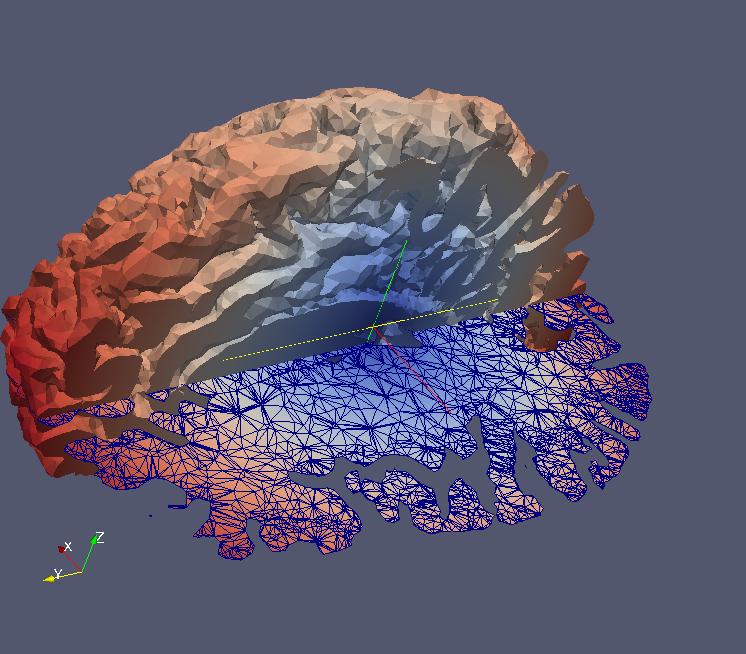
\includegraphics[scale=0.25]{chapters/elasticity/screen_shot.png}
  \end{center}
\caption{Deformation of the human brain during a cardiac cycle.}
\end{figure}


\section{Locking}
\label{el:lock}
The locking phenomena has nothing to do with the problem related to the rigid motions
studied in the previous section. Therefore, we consider locking in the simplest case possible
where we have homogenous Dirichlet conditions. In this case the elasticity equation
can be reduced to
\begin{eqnarray*}
-\mu \Delta u - (\mu + \lambda) \nabla \nabla\cdot u &=& f, \quad \mbox{in} \Omega,\\
                                                   u &=& 0, \quad \mbox{on} \partial \Omega. 
\end{eqnarray*}
The weak formulation of the problem then becomes:
Find $u \in H^1_0$ such that
\[
a(u,v) = f(v), \quad \forall v \in H^1_0, 
\]
where
\begin{eqnarray}
a(u,v) &=& \mu (\nabla u, \nabla v) + (\mu + \lambda) (\nabla \cdot u, \nabla \cdot v),\\
f(v)   &=& (f, v) .
\end{eqnarray}

The phenomen locking is a purely numerical artifact that arise when $\lambda \gg \mu$.
Roughly speaking, approximating $\nabla$ and $\nabla\cdot$ require different methods.
While vertices based approximations work fine for $\nabla$, edge based methods
are more natural for $\nabla\cdot$ since this operator relates directly
to the flux through the element edges.

For smooth functions, it can be verified directly that
\[
\Delta = \nabla\cdot\nabla = \nabla\nabla\cdot + \nabla\times \nabla\times
\]
where $\nabla\times$ is the curl operator.
Hence in $H_0^1$ we have 
\[
(\nabla u,\nabla v) = (\nabla \cdot u,\nabla \cdot v) + (\nabla \times u,\nabla \times v).
\]

Furthermore, it is well known (the Helmholz decomposition theorem) that any field in $L^2$ or $H^1$ can be decomposed
into a the gradient of a scalar potential (irrotational, curl-free vector field)
and the curl of scalar (a solenoidal, divergence-free vector field). That is,
\[
u = \nabla \phi + \nabla \times \psi, 
\]
where $\phi$ and $\psi$ are scalar fields that can be determined. 
Furthermore, 
\begin{eqnarray}
\nabla\cdot\nabla\times u = 0, \\
\nabla\times\nabla\cdot u = 0. 
\end{eqnarray}
This means that
\[
\nabla\nabla\cdot u = \left\{ \begin{array}{cc}
                          \Delta u & \mbox{ if } u \mbox{ is a gradient} \\
                                             0  & \mbox{ if } u \mbox{ is a curl}
                          \end{array} \right. 
\]
As the material becomes incompressible, when $\lambda\rightarrow\infty$ the gradient
part is being locked and $\phi$ tends to zero. However, the curl represented by $\psi$
remains unaffected. Vertex based finite elements such as Lagrange are poor
at distinguising between gradients and curls and tend to lock the complete solution.
Exercise \ref{ex:lock} investigates this phenomena numerically.

To avoid locking it is common to introduce a the quantity solid pressure,
$p = (\mu + \lambda) \nabla \cdot u$. Introducing this as a separate
unknown into the system we obtain the equations:
\begin{eqnarray*}
-\mu \Delta u - \nabla p = f, \\
\nabla\cdot u - \frac{1}{\mu + \lambda} p = 0 . 
\end{eqnarray*}
This system of equations is similar to the Stokes problem.
Hence, we may formulation a weak problems as follows.
Find $u\in H^1_0$ and $p \in L^2$ such that
\begin{eqnarray}
a(u,v) + b(p, v) &=& f(v) \forall v\in H^1 \\
b(u, q) - c(p,q) &=& 0, \forall q \in \R.
\end{eqnarray}
Here,
\begin{eqnarray}
a(u,v) &=& (\nabla u, \nabla v), \\
b(p, v) &=& (\nabla p, v), \\
c(p,q) &=& \frac{1}{\mu + \lambda}(p,q)\\
f(v) &=& (f,v).
\end{eqnarray}

The case when $\lambda\rightarrow\infty$ then represents the Stokes
problem as $\frac{1}{\mu + \lambda}\rightarrow 0$. Hence, for this
problem we know that stable discretizations can be obtained
as long as we have Stokes-stable elements like for instance Taylor--Hood.
We also remark that Stokes-stable elements handle any $\mu, \lambda$
because the $-c(p,q)$ is a negative term that only stabilize.
In fact, this problem is identical to the proposed penalty
method that was discussed for the Stokes problem. 



\begin{exercise}
\label{ex:sym:tensor}
Show that the inner product of a symmetric matrix $A$ and matrix $B$ equals
the inner product of $A$ and the symmetric part of $B$, i.e., that
$A:B$ = $A:B_S$, where $B_S = \frac{1}{2} (B + B^T)$. 
\end{exercise}

\begin{exercise}
Show that the term $\operatorname{div} \epsilon(u)$ in a weak setting may be written as $(\epsilon(u), \epsilon(v))$. Use the result of Exercise \ref{ex:sym:tensor}.   
\end{exercise}

\begin{exercise}
\label{ex:poissonbrezzi}
Show that the Brezzi conditions (\ref{remark1}-\ref{remark4}) for the singular problem of homogenous Neumann conditions for the Poisson problem \eqref{poisson:neu1}--\eqref{poisson:neu5}. Hint: use the following version of Poincare's lemma: 
\[
\|u-\bar{u}\|_0 \le C \|\nabla u \|_0, \quad \forall u \in H^1 .  
\]
Here, $\bar{u}=\frac{1}{|\Omega|}\int_\Omega u dx$. 
As always, the inf-sup condition is challenging, but notice that
\[
sup_{u\in V_h} \frac{b(u,q)}{\|u\|_{V_h}} \ge \frac{b(\bar{u},q)}{\|\bar{u}\|_{V_h}} .  
\]
\end{exercise}



\begin{exercise}
\label{ex:kornbrezzi}
Show that three of Brezzi conditions (\ref{remark1}-\ref{remark3}) for problem linear elasticity problem with pure Neumann conditions \eqref{el:lm:1}-\eqref{el:lm:2} are valid. Hint: use Korn's lemma for the coersivity.
As always, the inf-sup condition is challenging and we refer to \cite{kuchta2016singular}.
\end{exercise}

\begin{exercise}
\label{ex:lock}
We will consider the topic 'locking'. 
Consider the following equation on the domain $\Omega=(0,1)^2$: 
\begin{eqnarray}
-\mu \Delta u - \lambda \nabla \nabla \cdot u   &=& f \mbox{ in } \Omega, \\ 
        u &=& u_{analytical} \mbox{ on } \partial \Omega
\end{eqnarray}
where $u_{analytical}= (\frac{\partial \phi}{\partial y}, -\frac{\partial \phi}{\partial x})$ 
and $\phi= sin(\pi x y)$. Here, by construction, 
$\nabla \cdot u_{analytical} = 0$.  

\noindent
\textbf{a)} 
Derive an expression for $f$. Check that the expression is independent of $\lambda$. 

\noindent
\textbf{b)} 
Compute the numerical error for $\lambda=1, 100, 10000$
at $h=8, 16, 32, 64$ for polynomial order both 1 and 2.  

\noindent
\textbf{c)} 
Compute the order of convergence for different $\lambda$. 
Is locking occuring?

\end{exercise}

\chapter{Alternative Formulations}


\section{Introduction}

Most commonly, the basis for finite element methods has been the weak formulation as discussed in 
the previous chapters. But, with the introduction of neural networks and physics-informed networks, 
alternative formulations based on least square method principles have been made popular. Such formulations
have also been studied earlier, but has in general received little attention as compared with stdandard weak formulations.   
In this chapter we will therefore discuss different ways of formulating PDE problems. 
Let us for simplicity discuss elliptic problems with Dirichlet boundary conditions of the 
form: Find $u \in C^2(\Omega)$ given $f \in C^0(\Omega)$ of the form
\begin{align}
-\Delta u &= f \quad \mbox{ in } \Omega, \\ 
 u &= g \quad \mbox{ on } \Omega .  
\end{align}
The weak formulation: Find $u \in H^1_g(\Omega)$, given  $f \in H^{-1}(\Omega)$ such 
that 
\begin{align}
\label{weak:primal}
\int_\Omega \nabla u \cdot \nabla v \, dx = \int_\Omega f v \, dx, \quad \forall v\in H^1_0(\Omega),       
\end{align}
follows directly from Gauss-Green´s lemma, as we saw in Chapter \ref{ch:elliptic2}. 
We will refer to this formulation as the \emph{primal formulation}. 

The weak formulation may alternatively be derived from energy considerations. That is, 
consider the energy functional, 
\begin{align}
E (v, f) = \int_\Omega \frac{1}{2} (\nabla v)^2  - f v \, dx.   
\end{align}
The solution of \eqref{weak:primal} can equivalently be written as the minimizer of this energy functional. That is, 
\begin{align}
u = \argmin_{v \in H^1_g(\Omega) } E (v, f) .   
\end{align}
\kent{use u, v, $w_i$ such that both u and v can be expressed as a linear combination of $w_i$}
To see the relationship between the two formulations we need to be able to differentiate the functional $E$ with respect 
to functions $v$. Assume therefore that $H^1_g(\Omega)$ can be spanned by a basis $\{v_i\}^\infty_{i=1}$. Then 
a function can be expressed as $u=\sum_i u_i v_i$ and we notice directly that
\begin{align} 
\frac{\partial u }{\partial u_i } = v_i .  
\end{align} 
Hence, 
\begin{align} 
\frac{\partial E }{\partial u_i } = \int_\Omega \nabla u \cdot \nabla v_i - f v_i dx  .  
\end{align} 
Furthermore, clearly $E(v, f)$ is minimized when the derivative is zero, i.e. 
\begin{align} 
\frac{\partial E }{\partial u_i } = \int_\Omega \nabla u \cdot \nabla v_i - f v_i dx = 0  .  
\end{align} 
which corresponds to the weak formulation. 

\section{Least square formulation of primal formulation}

An alternative "energy"-like functional, based on least square principles that could be minimized would  
be  
\begin{align}
E_{LS} = \|-\Delta u - f\|_{L^2(\Omega)}
\end{align}
Again, we seek to find the minimizer
\begin{align}
u = \argmin_{v \in ? } E_{LS} (v, f) .   
\end{align}
We differentiate in order to find that 
\begin{align} 
\label{weak:primal:ls}
\frac{\partial E_{LS}}{\partial u_i} = \int_\Omega \frac{\partial}{\partial u_i} (-\Delta u - f)^2 \, dx  = \\  
2 \int_\Omega (-\Delta u - f) (-\Delta v_i) \, dx 
\end{align} 
By applying Gauss-Green´s lemma again we may again derive a corresponding strong formulation:
Find $u$ such that     
\begin{align}
\label{strong:primal:ls}
\Delta^2 u &= -\Delta f \quad \mbox{ in } \Omega, \\ 
 u &= g \quad \mbox{ on } \partial \Omega,   \\ 
 -\Delta u &= f \quad \mbox{ on } \partial \Omega .  
\end{align}

We refer \eqref{weak:primal:ls} and \eqref{strong:primal:ls} as the weak and strong formulation of the least square formulation of the
primal problem.  
We notice that both formulations requires more regularity than the standard weak formulation of the primal problem. In fact 
\eqref{strong:primal:ls} reguires $u \in C^4(\Omega)$ whereas   
\eqref{weak:primal:ls} is naturally posed in $H^2_g(\Omega)$.  

\section{The Mixed formulation}

To reduce the number of derivatives on the solution, a common 
trick is to splitt the original second order equation into 
two equations of first order. That is, we notice that
\begin{equation} 
\label{primal:mixed}
-\Delta u = f 
\end{equation} 
may be alternatively written as 
\begin{align}
\label{elliptic:mixed:1}
\psi = \nabla u, \\ 
\label{elliptic:mixed:2}
\nabla \cdot \psi = f . 
\end{align}
That is, inserting \eqref{elliptic:mixed:1} into the \eqref{elliptic:mixed:2} directly gives 
\eqref{primal:mixed}. Here, we notice that $\psi$ is a vector field while $u$ is a scalar field.  

Also this problem may be phrased as a minimization problem, although a constrained minimization problem. 
Let the energy be 
\[
E_{M}(\psi) = \int_\omega \frac{1}{2} \psi^2 \, dx  
\]
The the solution is  
\begin{align}
u = \argmin_{\nabla \cdot \psi = f  } E_{M} (v) .   
\end{align}
The constraint $\nabla \cdot v = f$ may be enforced using a Lagrange multiplier. Then the functional
becomes  
\[
L(v,\lambda, f) = \int_\Omega v^2 \, dx + \int_\Omega (\nabla \cdot v = g) \lambda  \, dx   
\]
and 
\begin{align}
u, \mu = \argmin_{v} \argmax_{\lambda} L(v, \lambda, f) .   
\end{align}
Again, we may differentiate (with respect to both $v$ and the Lagrange multiplier $\lambda$ to find the extremal points of $L$ 
as 
\begin{align}
 \frac{\partial L (u, \lambda)}{ \partial v} =  \int_\Omega v^2 \, dx + \int_\Omega (\nabla \cdot v = g) \lambda  \, dx   
\end{align}


 


\newpage

\backmatter
\printindex

\bibliographystyle{siamplain}
\bibliography{bibliography}

\end{document}





